\RequirePackage[l2tabu,orthodox]{nag}

% TODO: decide if one-sided/two-sided
%\documentclass[headsepline,footsepline,footinclude=false,fontsize=11pt,paper=a4,listof=totoc,bibliography=totoc,BCOR=12mm,DIV=12]{scrbook} % two-sided % original source stated: BCOR=12mm,DIV=12
\documentclass[headsepline,footsepline,footinclude=false,oneside,fontsize=11pt,paper=a4,listof=totoc,bibliography=totoc,DIV=12]{scrbook} % one-sided

% TODO: change citation style in settings
\PassOptionsToPackage{table,svgnames,dvipsnames}{xcolor}
%%%%%own packages inlcuded
\usepackage[verbose]{placeins} 

\usepackage{algorithm}
\usepackage{algpseudocode}
\usepackage{comment}
\usepackage{changepage}
\usepackage{booktabs}
%\usepackage[showframe=true]{geometry}
%%%%%own packages inlcuded

\usepackage[utf8]{inputenc}
\usepackage[T1]{fontenc}
\usepackage[sc]{mathpazo}
\usepackage[ngerman,english]{babel} % english is the same as american or USenglish
\usepackage[autostyle]{csquotes}
\usepackage[%
  backend=biber,
  url=true,
  style=numeric, % alphabetic, numeric
  sorting=none, % default == nty, https://tex.stackexchange.com/questions/51434/biblatex-citation-order
  maxnames=4,
  minnames=3,
  maxbibnames=99,
  giveninits,
  uniquename=init]{biblatex} % TODO: adapt citation style
\usepackage{graphicx}
\usepackage{scrhack} % necessary for listings package
\usepackage{listings}
\usepackage{lstautogobble}
\usepackage{tikz}
\usepackage{pgfplots}
\usepackage{pgfplotstable}
\usepackage{booktabs} % for better looking table creations, but bad with vertical lines by design (package creator despises vertical lines)
\usepackage[final]{microtype}
\usepackage{caption}
\usepackage[hidelinks]{hyperref} % hidelinks removes colored boxes around references and links
\usepackage{ifthen} % for comparison of the current language and changing of the thesis layout
\usepackage{pdftexcmds} % string compare to work with all engines
\usepackage{paralist} % for condensed enumerations or lists
\usepackage{subfig} % for having figures side by side
\usepackage{siunitx} % for physical accurate units and other numerical presentations
\usepackage{multirow} % makes it possible to have bigger cells over multiple rows in a table
\usepackage{array} % different options for table cell orientation
\usepackage{makecell} % allows nice manual configuration of cells with linebreaks in \thead and \makecell with alignments
\usepackage{pdfpages} % for including multiple pages of pdfs
\usepackage{adjustbox} % can center content wider than the \textwidth
\usepackage{tablefootnote} % for footnotes in tables as \tablefootnote
\usepackage{threeparttable} % another way to add footnotes as \tablenotes with \item [x] <your footnote> after setting \tnote{x} 


% https://tex.stackexchange.com/questions/42619/x-mark-to-match-checkmark
\usepackage{amssymb}% http://ctan.org/pkg/amssymb
\usepackage{pifont}% http://ctan.org/pkg/pifont
\newcommand{\cmark}{\ding{51}}%
\newcommand{\xmark}{\ding{55}}%


\usepackage[acronym,xindy,toc]{glossaries} % TODO: include "acronym" if glossary and acronym should be separated
\makeglossaries
\loadglsentries{pages/glossary.tex} % important update for glossaries, before document


\bibliography{bibliography}

\setkomafont{disposition}{\normalfont\bfseries} % use serif font for headings
\linespread{1.05} % adjust line spread for mathpazo font

% Add table of contents to PDF bookmarks
\BeforeTOCHead[toc]{{\cleardoublepage\pdfbookmark[0]{\contentsname}{toc}}}

% Define TUM corporate design colors
% Taken from http://portal.mytum.de/corporatedesign/index_print/vorlagen/index_farben
\definecolor{TUMBlue}{HTML}{0065BD}
\definecolor{TUMSecondaryBlue}{HTML}{005293}
\definecolor{TUMSecondaryBlue2}{HTML}{003359}
\definecolor{TUMBlack}{HTML}{000000}
\definecolor{TUMWhite}{HTML}{FFFFFF}
\definecolor{TUMDarkGray}{HTML}{333333}
\definecolor{TUMGray}{HTML}{808080}
\definecolor{TUMLightGray}{HTML}{CCCCC6}
\definecolor{TUMAccentGray}{HTML}{DAD7CB}
\definecolor{TUMAccentOrange}{HTML}{E37222}
\definecolor{TUMAccentGreen}{HTML}{A2AD00}
\definecolor{TUMAccentLightBlue}{HTML}{98C6EA}
\definecolor{TUMAccentBlue}{HTML}{64A0C8}

% Settings for pgfplots
\pgfplotsset{compat=newest}
\pgfplotsset{
  % For available color names, see http://www.latextemplates.com/svgnames-colors
  cycle list={TUMBlue\\TUMAccentOrange\\TUMAccentGreen\\TUMSecondaryBlue2\\TUMDarkGray\\},
}

% Settings for lstlistings

% Use this for basic highlighting
\lstset{%
  basicstyle=\ttfamily,
  columns=fullflexible,
  autogobble,
  keywordstyle=\bfseries\color{TUMBlue},
  stringstyle=\color{TUMAccentGreen}
}

% use this for C# highlighting
% %\setmonofont{Consolas} %to be used with XeLaTeX or LuaLaTeX
% \definecolor{bluekeywords}{rgb}{0,0,1}
% \definecolor{greencomments}{rgb}{0,0.5,0}
% \definecolor{redstrings}{rgb}{0.64,0.08,0.08}
% \definecolor{xmlcomments}{rgb}{0.5,0.5,0.5}
% \definecolor{types}{rgb}{0.17,0.57,0.68}

% \lstset{language=[Sharp]C,
% captionpos=b,
% %numbers=left, % numbering
% %numberstyle=\tiny, % small row numbers
% frame=lines, % above and underneath of listings is a line
% showspaces=false,
% showtabs=false,
% breaklines=true,
% showstringspaces=false,
% breakatwhitespace=true,
% escapeinside={(*@}{@*)},
% commentstyle=\color{greencomments},
% morekeywords={partial, var, value, get, set},
% keywordstyle=\color{bluekeywords},
% stringstyle=\color{redstrings},
% basicstyle=\ttfamily\small,
% }

% Settings for search order of pictures
\graphicspath{
    {logos/}
    {figures/}
}

% Set up hyphenation rules for the language package when mistakes happen
\babelhyphenation[english]{
an-oth-er
ex-am-ple
}

% Decide between
%\newcommand{\todo}[1]{\textbf{\textsc{\textcolor{TUMAccentOrange}{(TODO: #1)}}}} % for one paragraph, otherwise error!
%\newcommand{\done}[1]{\textit{\textsc{\textcolor{TUMAccentBlue}{(Done: #1)}}}} % for one paragraph, otherwise error!
% and
\newcommand{\todo}[1]{{\bfseries{\scshape{\color{TUMAccentOrange}[(TODO: #1)]}}}} % for multiple paragraphs
\newcommand{\done}[1]{{\itshape{\scshape{\color{TUMAccentBlue}[(Done: #1)]}}}} % for multiple paragraphs
% for error handling of intended behavior in your latex documents.

\newcommand{\tabitem}{~~\llap{\textbullet}~~}

\newcolumntype{P}[1]{>{\centering\arraybackslash}p{#1}} % for horizontal alignment with limited column width
\newcolumntype{M}[1]{>{\centering\arraybackslash}m{#1}} % for horizontal and vertical alignment with limited column width
\newcolumntype{L}[1]{>{\raggedright\arraybackslash}m{#1}} % for vertical alignment left with limited column width
\newcolumntype{R}[1]{>{\raggedleft\arraybackslash}m{#1}} % for vertical alignment right with limited column width

% TODO: change thesis information
\newcommand*{\getUniversity}{Technische Universität München}
\newcommand*{\getFaculty}{Department of Informatics}
\newcommand*{\getTitle}{Intelligent Ball Screw Fault Diagnosis using Deep Learning based Domain Adaption and Transfer Learning}
\newcommand*{\getTitleGer}{Intelligente Fehlerdiagnose von Kugelgewinden mittels Deep Learning, basierend auf Domain Adaption und Transfer Learning}
\newcommand*{\getAuthor}{Fabian Kolb}
\newcommand*{\getDoctype}{Master's Thesis in Informatics: Robotics, Cognition, Intelligence}
\newcommand*{\getSupervisor}{Zäh Michael; Prof. Dr.-Ing.}
\newcommand*{\getAdvisor}{Benker Maximilian; M.Sc.}
\newcommand*{\getSubmissionDate}{15.Sept.2022}
\newcommand*{\getSubmissionLocation}{Munich}

%%%%% own inlcuded

\DeclareSourcemap{
                \maps[datatype=bibtex]{
                               % remove fields that are always useless
                               \map{
                                               \step[fieldset=abstract, null]
                                               \step[fieldset=pagetotal, null]
                                               \step[fieldset=month, null]
                               }
                               % remove URLs for types that are primarily printed
                               \map{
                                               \pernottype{software}
                                               \pernottype{online}
                                               \pernottype{report}
                                               \pernottype{techreport}
                                               \pernottype{standard}
                                               \pernottype{manual}
                                               \pernottype{misc}
                                               \step[fieldset=url, null]
                                               \step[fieldset=urldate, null]
                               }
                               \map{
                                               \pertype{inproceedings}
                                               \pertype{article}
                                               % remove mostly redundant conference information
                                               %\step[fieldset=venue, null]
                                               %\step[fieldset=eventdate, null]
                                               %\step[fieldset=eventtitle, null]
                                               % do not show ISBN for proceedings
                                               \step[fieldset=isbn, null]
                                               \step[fieldset=issn, null]
                                               % Citavi bug
                                               %\step[fieldset=volume, null]
                               }
                               \map{
                                               \pertype{book}
                                               \pertype{inbook}
                                               \pertype{incollection}
                                               % remove mostly redundant conference information
                                               %\step[fieldset=venue, null]
                                               %\step[fieldset=eventdate, null]
                                               %\step[fieldset=eventtitle, null]
                                               % do not show ISBN for proceedings
                                               \step[fieldset=doi, null]
                                               % Citavi bug
                                               %\step[fieldset=volume, null]
                               }
                }
}
%%%%% own inlcuded

\begin{document}

% TODO: decide on used language
%\selectlanguage{ngerman}
\selectlanguage{english}

% Set page numbering to avoid "destination with the same identifier has been already used" warning for cover page.
% (see https://en.wikibooks.org/wiki/LaTeX/Hyperlinks#Problems_with_Links_and_Pages).
\pagenumbering{alph}
\begin{titlepage}
  % HACK for two-sided documents: ignore binding correction for cover page.
  % Adapted from Markus Kohm's KOMA-Script titlepage=firstiscover handling.
  % See http://mirrors.ctan.org/macros/latex/contrib/koma-script/scrkernel-title.dtx,
  % \maketitle macro.
  \oddsidemargin=\evensidemargin\relax
  \textwidth=\dimexpr\paperwidth-2\evensidemargin-2in\relax
  \hsize=\textwidth\relax

  \centering

  \IfFileExists{logos/tum.pdf}{%
    
\includegraphics[height=20mm]{logos/tum.pdf}
  }{%
    \vspace*{20mm}
  }

  \vspace{5mm}
  {\huge\MakeUppercase{\getFaculty{}}}\\

  \vspace{5mm}
  {\large\MakeUppercase{\getUniversity{}}}\\

  \vspace{20mm}
  {\Large \getDoctype{}}

  \vspace{15mm}
  \makeatletter
  \ifthenelse{\pdf@strcmp{\languagename}{english}=0}
  {\huge\bfseries \getTitle{}}
  {\huge\bfseries \getTitleGer{}}
  \makeatother

  \vspace{15mm}
  {\LARGE \getAuthor{}}

  \IfFileExists{logos/faculty.png}{%
    \vfill{}
    
\includegraphics[height=20mm]{logos/faculty.png}
  }{}
\end{titlepage}


\frontmatter{}

\begin{titlepage}
  \centering

  \IfFileExists{logos/tum.pdf}{%
    
\includegraphics[height=20mm]{logos/tum.pdf}
  }{%
    \vspace*{20mm}
  }

  \vspace{5mm}
  {\huge\MakeUppercase{\getFaculty{}}}\\

  \vspace{5mm}
  {\large\MakeUppercase{\getUniversity{}}}\\

  \vspace{20mm}
  {\Large \getDoctype{}}

  \makeatletter
  \vspace{15mm}
  \ifthenelse{\pdf@strcmp{\languagename}{english}=0}
  {
  {\huge\bfseries \getTitle{}}

  \vspace{10mm}
  {\huge\bfseries \foreignlanguage{ngerman}{\getTitleGer{}}}
  }
  {
  {\huge\bfseries \getTitleGer{}}

  \vspace{10mm}
  {\huge\bfseries \foreignlanguage{english}{\getTitle{}}}
  }
  \makeatother

  \vspace{15mm}
  \begin{tabular}{l l}
    Author:          & \getAuthor{} \\
    Supervisor:      & \getSupervisor{} \\
    Advisor:         & \getAdvisor{} \\
    Submission Date: & \getSubmissionDate{} \\
  \end{tabular}

  \IfFileExists{logos/faculty.png}{%
    \vfill{}
    
\includegraphics[height=20mm]{logos/faculty.png}
  }{}
\end{titlepage}

\cleardoublepage{}

\thispagestyle{empty}
\vspace*{0.8\textheight}
\noindent
\makeatletter
\ifthenelse{\pdf@strcmp{\languagename}{english}=0}
{I confirm that this \MakeLowercase{\getDoctype{}} is my own work and I have documented all sources and material used.}
{Ich versichere, dass ich diese \getDoctype{} selbstständig verfasst und nur die angegebenen Quellen und Hilfsmittel verwendet habe.}
\makeatother

\vspace{15mm}
\noindent
\getSubmissionLocation{}, \getSubmissionDate{} \hspace{50mm} \getAuthor{}

\cleardoublepage{}

\makeatletter
\ifthenelse{\pdf@strcmp{\languagename}{english}=0}
{\addcontentsline{toc}{chapter}{Acknowledgments}}
{\addcontentsline{toc}{chapter}{Danksagungen}}
\makeatother
\thispagestyle{empty}

\vspace*{20mm}

\begin{center}
\makeatletter
\ifthenelse{\pdf@strcmp{\languagename}{english}=0}
{\usekomafont{section} Acknowledgments}
{\usekomafont{section} Danksagungen}
\makeatother
\end{center}

\vspace{10mm}

%TODO: Acknowledgments

\cleardoublepage{}
 % TODO: if you don't have anyone to thank for or don't wish to publish it, comment this line out.
\chapter{\abstractname}

%TODO: Abstract
In order to remain competitive in the ongoing globalization, companies are forced to optimize their productions and processes. Using modern smart technologies like Internet of Things (IoT) and Machine to machine communication (M2M) advances the digitization and automation in production facilities. The immense amount of generated data offers great opportunities for Predictive Maintenance approaches. By analysing machine and production data, machines can be proactively maintained, thereby increasing quality standards and productivity. Since ball screws are one of the most common parts in industrial machines, their health monitoring is especially interesting. Due to strong abrasion ball screws change a lot during lifetime.
Therefore, a strong shift in the data distribution can be observed between the working conditions. This makes the fault diagnosis problem more challenging. In order to tackle this problem deep-learning based domain adaption approaches, which are common in the Computer Vision community are promising. In this work, the applicability of such approaches to the given predictive maintenance problem is investigated. 




\makeatletter
\ifthenelse{\pdf@strcmp{\languagename}{english}=0}
{\renewcommand{\abstractname}{Kurzfassung}}
{\renewcommand{\abstractname}{Abstract}}
\makeatother

\chapter{\abstractname}

%TODO: Abstract in other language
\begin{otherlanguage}{ngerman} % TODO: select other language, either ngerman or english !
Um in der fortschreitenden Globalisierung wettbewerbsfähig zu bleiben, sind Unternehmen gezwungen, ihre Produktionen und Prozesse zu optimieren. Der Einsatz moderner intelligenter Technologien wie Internet of Things (IoT) und Machine-to-Machine-Kommunikation (M2M) treibt die Digitalisierung und Automatisierung in der Produktion weiter voran. Die dabei generierten Datenmengen ermöglichen moderne für Predictive Maintenance-Ansätze. Durch die Analyse von Maschinen- und Produktionsdaten können Maschinen proaktiv gewartet werden, um dadurch die Qualitätsstandards und Produktivität zu erhöhen. Da Kugelgewindetriebe  in Industriemaschinen häufig verbaut werden, ist deren Zustandsüberwachung besonders interessant. Durch den hohen Verschleiß verändern sich Kugelgewindetriebe über ihrer Lebensdauer stark. Zwischen den Betriebszuständen ist deshalb eine starke Verschiebung in der Datenverteilung zu beobachten. Dies macht die Fehlerdiagnose herausfordernd. Deep-Learning-basierte Domain-Adaption Ansätze, die in der Computer-Vision-Community verbreitet sind, sind daher vielversprechend. In dieser Arbeit wird die Anwendbarkeit solcher Ansätze für das gegebene Predictive Maintenance Probelem untersucht. 


\end{otherlanguage}


% Undo the name switch
\makeatletter
\ifthenelse{\pdf@strcmp{\languagename}{english}=0}
{\renewcommand{\abstractname}{Abstract}}
{\renewcommand{\abstractname}{Kurzfassung}}
\makeatother
\microtypesetup{protrusion=false}
\tableofcontents{}
\microtypesetup{protrusion=true}

\mainmatter{}

% !TeX root = ../main.tex
% Add the above to each chapter to make compiling the PDF easier in some editors.

\chapter{Introduction}\label{chapter:introduction}
Modern sensors, data infrastructures and traditional as well as machine learning algorithms have revolutionized the industry. As a key role in modern production facilities, Prognostic and Health Managment (PHM) applications have fully embraced the Big Data revolution. By analyzing production and machine data, future machine failures or working conditions can be predicted. This is especially helpful to prevent or at least warn employees about sudden and unexpected problems with production machines. The idea of PHM is to reduce the downtime of whole production lines \cite{ZHAO2019213}. Today's globalized world demands efficient internal processes and production strategies from companies. Therefore, the need for reliable PHM applications grew recently. Due to this increasing interest also the research focuses more and more on related topics. This thesis evaluates PHM approaches on a real production use case.

\section{Problems of Prognostics and Health Management for ball screw drives}
In a wide range of industrial machines, ball screws are used, which translate rotatory into linear motion with high precision. During longtime use, degradation lowers the stiffness within the ball screw components. This leads to an inaccurate position movement, which lowers the precision of the machine and therefore the production quality. In the worst case, a whole machine failure may occur. For this reason, tracking the ball screw health condition is of great importance. In recent years, PHM research mainly focused on rolling bearings and gearboxes. Since industrial machines and components have different operation conditions, working cycles and sensor installations, requirements for PHM algorithms vary. The transferability of PHM algorithms is limited and does usually require adjustments. However, intelligent data-driven methods have been successfully developed. Unfortunately, a lot of these approaches assume the training and testing data to be from the same data distribution. In reality, this is not the case. Since the operating conditions, component degradation and machine settings may change, the fault characteristics of the machines do also change. Fault diagnosis systems which are trained on a limited amount of data, which represents the machine fault characteristics partially, usually can't generalize well on the testing data with changed fault characteristics. Consequently, such diagnosis systems show unsatisfactory performance when being applied in real industrial scenarios over long periods of time. This phenomenon is called domain shift problem \cite{AZAMFAR2020103932}. In order to compensate the domain shift problem in health monitoring tasks, domain adaption and transfer learning approaches can be applied. These methods attempt to minimize the distribution discrepancy that occurs when recording machine data over a long period of time and is caused by the changed fault characteristics. 

\section{Traditional Prognostics and Health Management Approaches}
As shown in fig. \ref{fig:hand_crafted_features_physical_models_deep_learning} health monitoring is traditionally restricted to physical-based and conventional data-driven approaches. In the context of PHM, physical laws sound promising to explain the underlying complexity of a machine. These models are especially attractive since they don't require any historical fault data to make predictions about the health condition of a machine \cite{AN201942}. If the physics projected on the data doesn't include all relevant machine aspects as well as noise and perturbation, the performance of such approaches is reduced. With the upcoming modern sensors, networks and computing systems, data-driven approaches became more and more relevant for real world scenarios. In conventional data-driven approaches, traditional hand-crafted features are used to extract expressive information from the data in a first step. Subsequently, a shallow classifier predicts the corresponding health condition state for the samples. The just mentioned methods suffer from three problems. Firstly, in complex real-world scenarios, establishing physical-based models or conventional hand-crafted features is quite a laborious task and expects a lot of experience. Secondly, an on-line model update is not possible. Thirdly, the physical-based models and hand-crafted features are restricted to the application of interest and suffer from bad transferability. The limited flexibility and effectiveness of the two traditional approaches are responsible for the growing interest in deep learning based PHM. Deep neural networks can capture relations within complex and high-dimensional data. By using multiple layers, neural networks can progressively extract features with different levels of abstraction. The automatic learning makes neural networks easily adjustable to different problems. The popularity of neural networks exploded especially due to the increasing amount of data, computational power \cite{ZHAO2019213} \cite{AZAMFAR2020103932}. Especially, when using 

\begin{figure}[H]
  \centering
  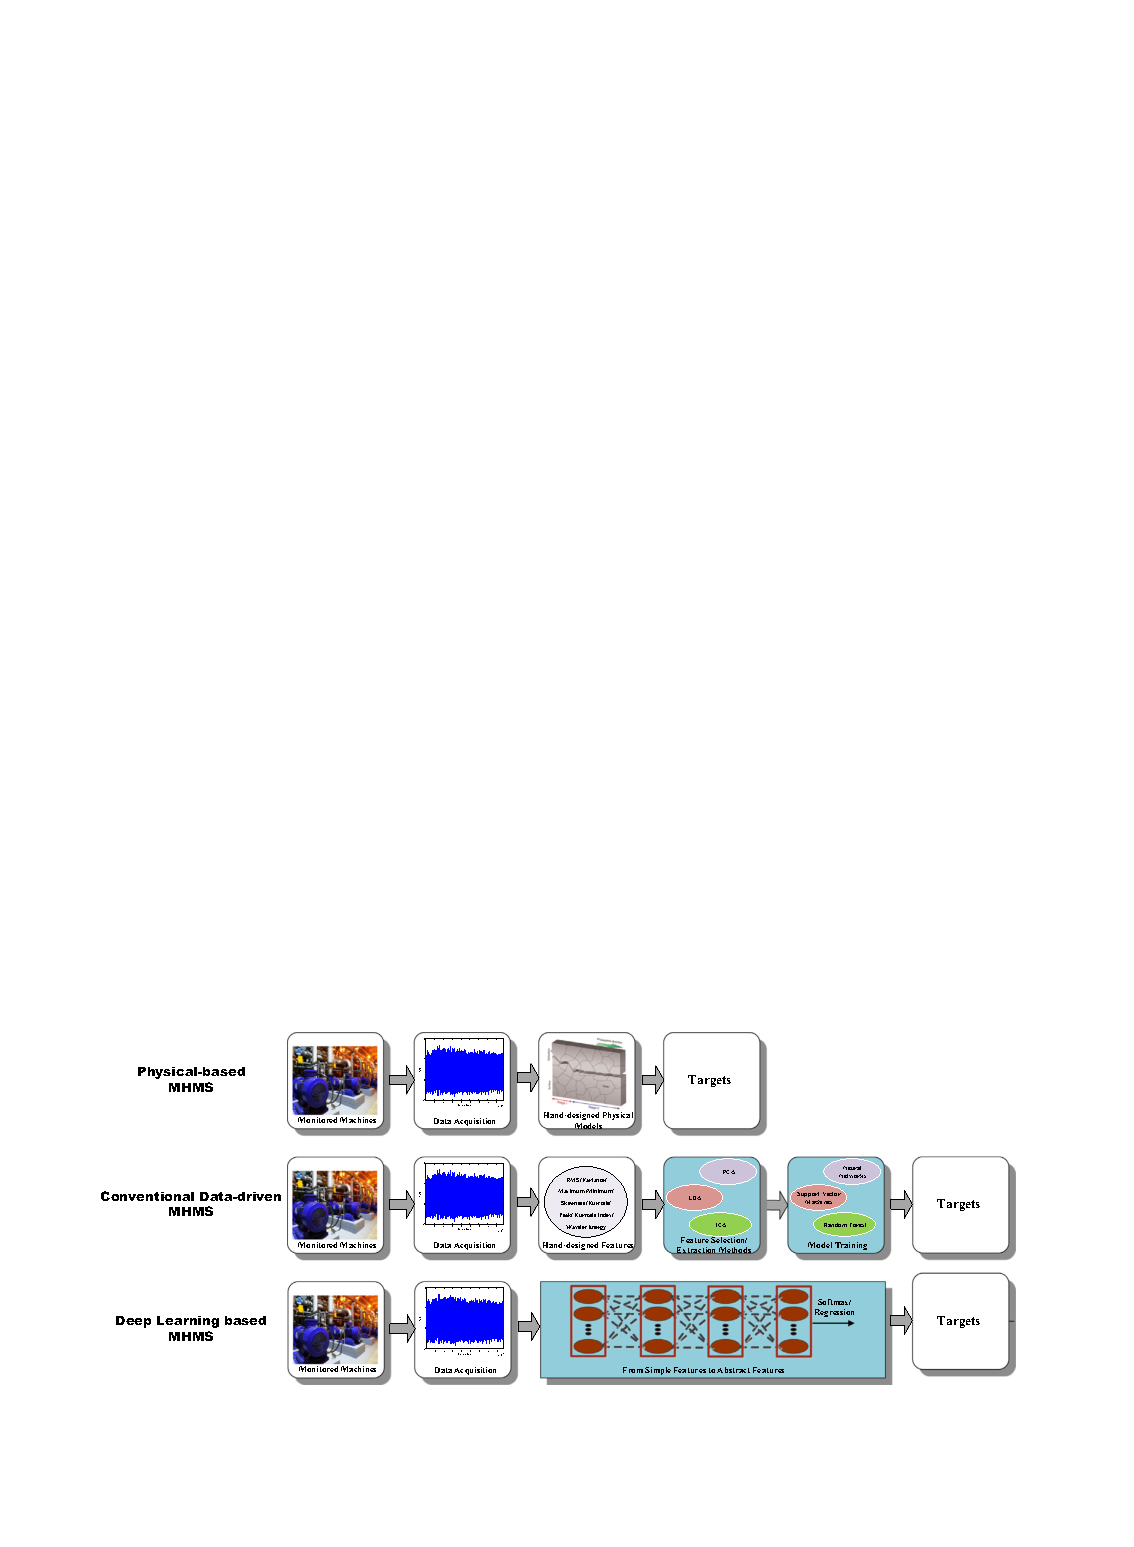
\includegraphics[width=1\textwidth]{hand_crafted_features_physical_models_deep_learning.pdf}
  \caption {Physical Models, Conventional Data-driven Models and Deep Learning Models for predictive maintenance \cite{ZHAO2019213}} \label{fig:hand_crafted_features_physical_models_deep_learning}
\end{figure}
\chapter{Theory}\label{chapter:theory}

\section{Neural network}

Inspired from the nature, neural networks try to imitate the function of human brains. Deep Learning is a specific branch of machine learning. Due to modern technologies like IoT gigantic amounts of data are recorded and processed in order to make production more efficient and reliable. The increased amount of data and computational power makes Deep Learning applications more and more popular. Neural networks are hierarchically structured non-linear processing layers which try to learn hierarchical representations of data. Due to the increasing interest the deep learning community recently came up with various new deep learning architectures. In the following some of those are explained more in detail

\subsection{Neural Network Architecture}
Neural networks consist of neurons which are layered in a hierarchical architecture. The neurons of consecutive layers are connected through weights and biases. During the optimization of the model the weights and biases are updated. Fig. \ref{fig:neural_network_overview} gives an overview of how neurons are arranged in a fully-connected layered architecture. Each neuron from layer i is connected with all neurons from layer i+1 and shares information with them.

\begin{figure}[htpb]
  \centering
  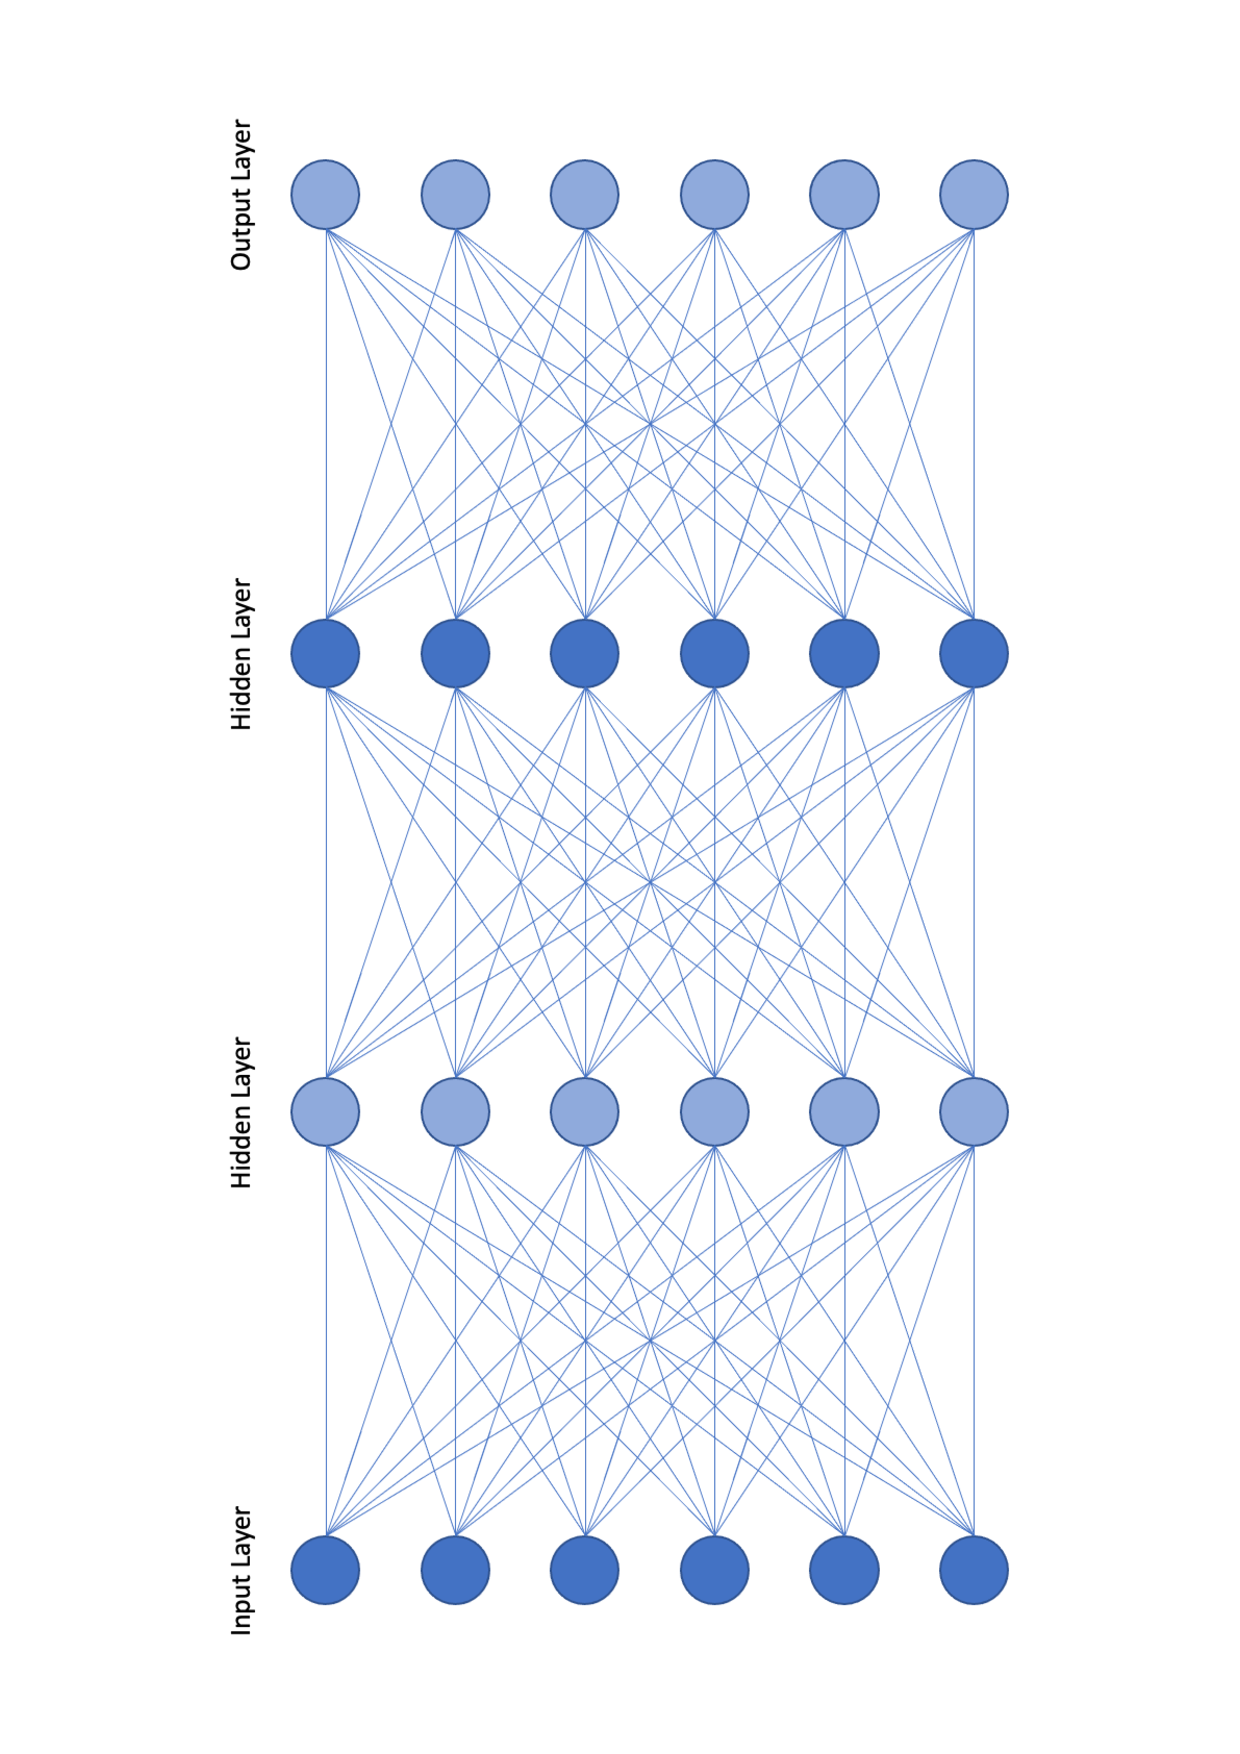
\includegraphics[width=0.7\textwidth, angle =-90]{neural_network_overview.pdf}
  \caption {Layer overview neural network}
  \label{fig:neural_network_overview}
\end{figure}

The input of a neuron is calculated from the sum of all previous neuron's outputs and one bias. Afterwards an activation function is applied to give the neural network a non-linear property. Standard multilayer feedforward networks with even one single hidden layer and an arbitrary bounded and non-constant activation function are universal approximators. This means that a wide variety of functions can be represented by the neural network when given appropriate weights \cite{HORNIK1991}. Without activation functions neural network could only make linear assignments of inputs x to outputs y. With rising data complexity the demand for a "non-linear" mapping from x to y is increasing. Without a non-linearity the neural network with several hidden layers can just learn the same functions as those with just one hidden layer. Such a neural network would not be able to mathematically realise complex relationships in the data. Fig. \ref{fig:neural_network_optimization} shows the forward- and backwardpropagation in a neural network at the example of one single neuron. First the outputs of the neurons $i$ from the previous layers $l-1$ which are connected with the neuron of interest $j$ in layer $l$ are summed up together with a bias $b_{j}$. The resulting logits $z_{j}$ are then processed by the activation function $\phi$. Different activation functions can be used throughout the network. After passing several consecutive hidden layers a loss function evaluates the prediction with the ground truth label in the end of the network.

\subsection{Activation Function}
Different problems and network layers require different activation functions. Typical activation functions are tanh, sigmoid and ReLU in the hidden as well as linear, logistic (sigmoid) and softmax in the final layers of the network \cite{Brownlee2021}. Linear final layers are used for regression problems, whereas sigmoid and softmax functions are typical for classification problems. The sigmoid function is used for binary and softmax for multiclass classification. In general the softmax function is an extension of the sigmoid function to the multiclass case, which can be proofed easily. The softmax and sigmoid functions normalize the network output to a probability distribution over the predicted output classes.  Deciding for the activation functions in the hidden layers is a little more difficult. All just mentioned functions have different characteristics which lead to individual advantages and disadvantages. The sigmoid and tanh function look pretty similar. Both squeeze the inputs in values between -1 and 1. Both functions can suffer from the vanishing gradient problem since the derivative of these functions is close to zero for very big or small inputs. A solution for that is the ReLU function which solves that problem but is limited due to the mapping of negative inputs to zero (dead ReLU) \cite{Brownlee2021}. In table \ref{tab:activation_functions} some of the most popular activation functions are described. \newline
\newline



\begin{tabular}{ c c c c }
\hline 
Formula & Formulation s(x) & Derivative $\frac{ds(x)}{dx}$ & Function output range \\ \hline                        
ReLU &   \begin{cases} 0 & \text{, for }x < 0\\
	x & \text{, for }x \geqslant 0 \end{cases} & \begin{cases} 0 & \text{, for }1 < 0\\
	1 & \text{, for }x \geqslant 0 \end{cases} & [ 0, \infty)\\

\rule{0pt}{5ex}%  EXTRA vertical height 

Leaky ReLU &   \begin{cases} \alpha x & \text{, for }x < 0\\
	x & \text{, for }x \geqslant 0 \end{cases} & \begin{cases} \alpha & \text{, for }1 < 0\\
	1 & \text{, for }x \geqslant 0 \end{cases} & (-- \infty, \infty)\\

\rule{0pt}{5ex}%  EXTRA vertical height 

ELU &   \begin{cases} \alpha(e^{x} - 1) & \text{, for }x < 0\\
	x & \text{, for }x \geqslant 0 \end{cases} & \begin{cases} \alpha e^{x} & \text{, for }x < 0\\
	1 & \text{, for }x \geqslant 0 \end{cases} & [−\alpha, \infty)\\
	
\rule{0pt}{5ex}%  EXTRA vertical height 
	
Sigmoid & $\frac{1}{1+e^{-x}}$ & $\frac{e^{-x}}{(1+e^{-x})^{2}}$ & (0,1)\\

\rule{0pt}{5ex}%  EXTRA vertical height 

Softmax & $\frac{e^{x_{i}}}{\sum_{j=1}^{K} e^{x_{j}}}$ & $\frac{e^{-x}}{(1+e^{-x})^{2}}$ & (0,1)\\

\rule{0pt}{5ex}%  EXTRA vertical height 

tanh & $\frac{e^{2x}-1}{e^{2x}+1}$ & $1-tanh^{2}(x)$ & (-1,1) \\
\hline  
\label{tab:activation_functions}

\end{tabular}
\captionof{table}{Overview activation functions}




\subsection{Optimization}
When training neural networks one has to decide for a loss function and an optimizer. 

\subsubsection{Loss}
The loss function acts as a model evaluation criterion and the optimizer is responsible for adapting the model accordingly. Deep Learning models can be divided into two groups: (1) regression tasks and (2) classification tasks. In a regression problem the goal is to learn a mapping function from input variables to a continuous output variable. Contrairwise, in a classification problem the model aims to predict the class label from the input variables \cite{ShilohPerl2020}. Typically Mean Square Error (MSE) , shown in eq. \ref{eq:MSE} , is used for regression problems:

\begin{equation}
L(X) =  \sum_{x}(\hat{y}(x)-y(x))^2
\label{eq:MSE}
\end{equation}

where $y(x)$ is the ground truth and $\hat{y}(x)$ the predicted class label \cite{ShilohPerl2020}. The Cross Entropy Loss, shown in eq. \ref{eq:CE} is rather more used for classification problems: 

\begin{equation}
L(X) = \sum_{x} y(x) log(p(x))
\label{eq:CE}
\end{equation}
where p(x) is the predicted probability of the sample $x$ belonging to the ground truth class $y(x)$ \cite{ShilohPerl2020}.

\subsection{Training Loop}
The weights and biases of the model are adapted such that the loss is minimized. This optimization takes place in a two stage process: (a) feed-forward pass of the input data throughout the model and calculating corresponding neuron outputs and the loss from the predicted and ground-truth labels; followed by (b) backward pass of the loss throughout the model and updating the model weights accordingly. Iteratively this process is performed to optimize the model performance. During the backward pass the gradients of the loss with respect to the network weights is calculated and used to update the weights and biases of the network. The process is visualized in fig. \ref{fig:neural_network_optimization} (green: forward pass, red: backward pass). All the weights and biases are updated recursively by calculating the gradients of every layer, starting from the final and ending at the input layer. Using the chain rule, different partial derivatives of the network can be concatenated. Eq. \ref{chain_rule} shows the chain rule used during backpropagation:
\begin{equation}
 \frac{\delta L_{i}}{\delta w_{i}} = \frac{\delta L_{i}}{\delta \hat{y_{i}}} * \frac{\delta \hat{y_{i}}}{\delta z_{i}} * \frac{\delta z_{i}}{\delta w_{i}}, 
 \label{chain_rule}
\end{equation}
where $\frac{\delta L_{i}}{\delta \hat{y_{i}}}$ is the derivative of the loss with respect to the output of the activation function of the last layer, $\frac{\delta \hat{y_{i}}}{\delta z_{i}}$ is the derivative of the activation function and $\frac{\delta z_{i}}{\delta w_{i}}$ is the derivative of the logits $z_{i}$ with respect to the weights and biases \cite{ShilohPerl2020}.

\begin{figure}[htpb]
  \centering
  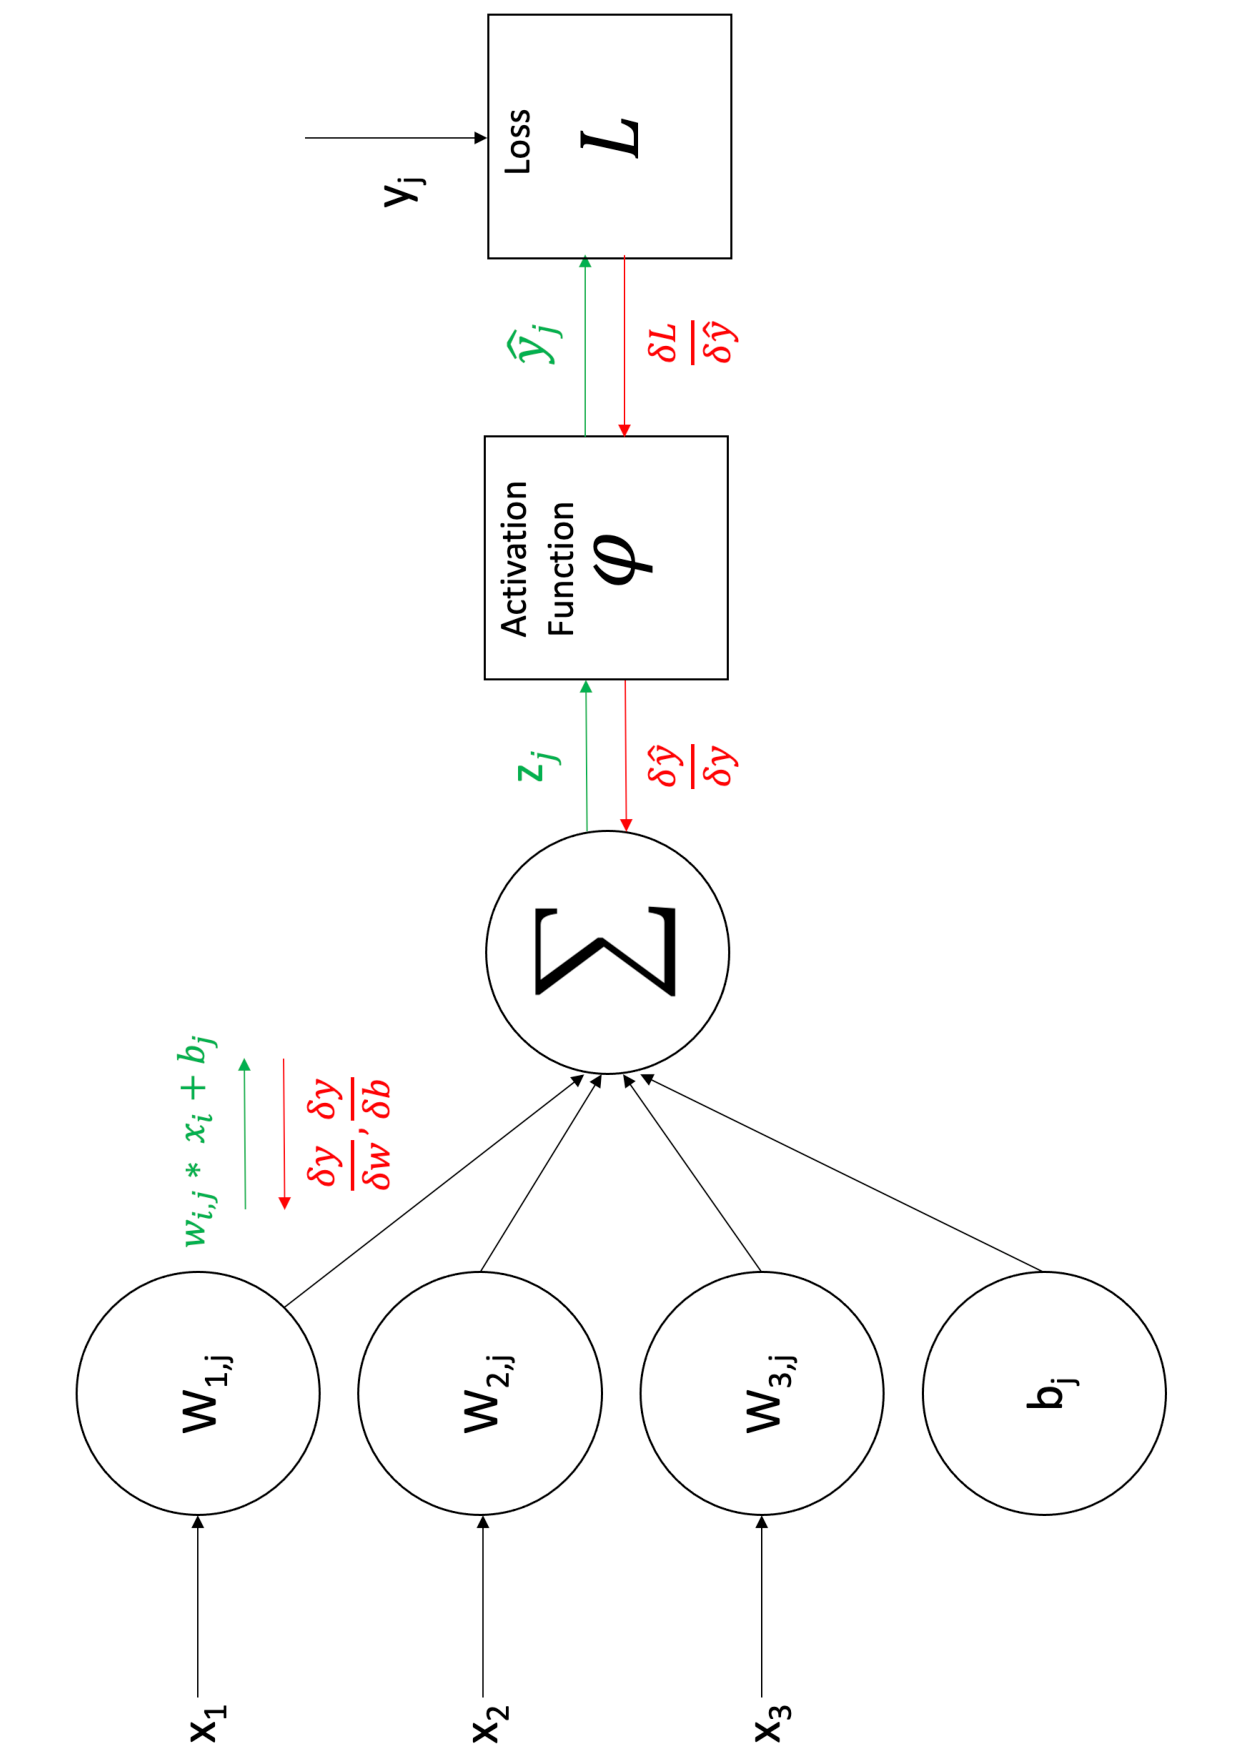
\includegraphics[width=0.7\textwidth, angle = -90]{neural_network_optimization.pdf}
  \caption {Optimization of neural network}
  \label{fig:neural_network_optimization}
\end{figure}


\subsection{Optimizer}
Calculating the gradient for the whole dataset is computationally expensive. A common practice is therefore to separate the dataset in several subsets, so called mini-batches. For each mini-batch the corresponding gradients are calculated and the model is updated accordingly. This process is repeated for all the mini-batches retrieved from the dataset. Each cycle of training over the whole dataset is called an epoch and in every cycle. When the loss converges the training can be terminated. Despite convergence an optimal solution is not assured since the most neural network problems are not convex \cite{ShilohPerl2020}.


Applying gradient descent based optimizer, the weights and biases are updated with a step in the negative direction of the derivative:

\begin{equation}
  w_{new} = w_{old} - \eta \frac{\delta L}{\delta w_{old}},
\end{equation}
where $w_{old}$ are the old, $w_{new}$ are the new model parameters, $\eta$ is the learning rate and $\frac{\delta L}{\delta w_{old}}$ is the derivative of the loss with respect to the current model weights \cite{ShilohPerl2020}. 
Most optimizer rely only on the gradients (first order methods). Using second-order methods do generally converge faster but also require the computation of the Hessian. This is especially expansive for big datasets and models. For this reason Stochastic Gradient Descent is an optimization option which randomly picks samples to optimize the model. For this reason Stochastic Gradient Descent (SGD) is used, which calculates the gradient for single randomly picked samples from the dataset. Since the choice of these samples is random, the optimization suffers from instability and fluctuation. Instead of regular SGD one can use mini-batch gradient descent. This is a compromise between the regular SGD and gradient descent method. The gradient and model update is neither performed for a single sample nor for the whole dataset, but it is performed on a small randomly picked subset of the dataset, which accelerates the convergence of the training.\newline
\newline
\textbf{Momentum}\newline
In order to accelerate and stabilize the optimization one can also include historical gradients. First and second Momentum is a method that helps accelerate SGD in the relevant direction and dampens oscillations \cite{ShilohPerl2020} . Instead of updating with a fixed stepsize in the direction of the negative gradient one can use first and second momentum to adapt the stepsize of the optimization in the different dimensions. In the following four different optimizer which use first, second momentum or a combination of those. An optimization with first momentum works as follows:

\begin{equation}
  \begin{aligned}
  v_{t} = & \gamma v_{t-1} +  \eta \nabla_{\theta}L(W_{t-1}) &\\
  W_{t} = &W_{t-1} - v_{t},
  \end{aligned}
  \label{eq:moment}
\end{equation}

where $M_{t}$ is the momentum, which calculates a moving average over the past gradients, $\nabla_{\theta}L(W_{t})$ is the derivative of the loss with respect to the current model weights, $\beta$ defines the relationship between current gradient and momentum in the moving average, $W_{t-1}$ are the current and $W_{t}$ the updated model weights \cite{Ruder2016}.\newline
\newline
\textbf{Nesterov accelerated gradient (NAG)}\newline
Another well known optimizer of this kind is NAG which works just like described in  \ref{eq:moment}. The only difference is that that the gradient is not estimated for the current, but for some pre-udpated model weights. In a first step the gradient is calculated for the old model weights, which are updated with the momentum from the previous iteration $\nabla_{\theta}L( W_{t-1} - \gamma v_{t-1})$. In a second step the current model weights  are updated with the moving average of the momentum and gradient as described in \label{eq:moment} \cite{Ruder2016}.\newline
\newline
\textbf{Adagrad}\newline
Instead of using first momentum, Adagrad builds a moving average of the the past squared gradients (second momentum):

\begin{equation}
  \begin{aligned}
  W_{t} = W_{t-1} - \frac{\eta}{\sqrt[2]{G_{t}+ \epsilon}} \bigodot \nabla_{\theta}L(W_{t-1}),
  \end{aligned}
  \label{eq:Adagrad}
\end{equation}

where  $W_{t-1}$ are the current and $W_{t}$ the updated model weights, $\nabla_{\theta}L(W_{t})$ is the derivative of the loss with respect to the current model weights, $G_{t}$ is second momentum and $\epsilon$ denotes a small quantity which prevents the division by zero  \cite{Ruder2016}.\newline
\newline
\textbf{Adaptive Moment Estimation (ADAM)}\newline
The Adam is one of the most popular optimizer. ADAM combines the idea of first and second momentum: 
\begin{equation}
  \begin{aligned}
   &m_{t} =  \beta_{1} m_{t-1} +  (1-\beta_{1}) \nabla_{\theta}L(W_{t-1}) &\\
    &v_{t} =  \beta_{2} v_{t-1} +  (1-\beta_{2}) \nabla_{\theta}L^{2}(W_{t-1}) &\\
    &\hat{m}_{t} = \frac{m_{t}}{1-\beta_{1}^{t}}&\\
    &\hat{v}_{t} = \frac{v_{t}}{1-\beta_{2}^{t}}&\\
   & W_{t} = W_{t-1} - \frac{\eta}{\sqrt[2]{\hat{v}_{t} + \epsilon}}\hat{m}_{t}, &\\
  \end{aligned}
  \label{eq:moment}
\end{equation}

where $m_{t}$ and $v_{t}$ are the first and second momentum, $\hat{m}_{t}$ and $\hat{v}_{t}$ are the bias-corrected first and second moment estimates, $\beta_{1}$ and $\beta_{2}$ are the weighting factors for the moving average and $W_{t-1}$ and  $W_{t}$ are the current and updated model weights \cite{Ruder2016}.



\section{Convolutional Neural Network (CNN)}

Equally to regular neural networks CNNs consist of several neurons embedded in a fixed architecture. CNNs focus on processing images and therefore the architecture is set up such that dealing with images is optimized. In CNNs the neurons are structured in layers just like in normal neural networks. In regular networks the neurons of one layer are are organized in one dimension and in CNNs in three dimensions (height, width, depth).

The functionality of CNNs are visualized in \ref{fig:CNN_overview}. One can identify four main compounts of a CNN, which are described more detailed in the following:

\begin{itemize}
    \item [1.] Data which is organized in a structured 1D or 2D form is fed into the CNN as input layer. Each element in this structure is called a pixel. A pixel contains a specific value and position in the structure. 
    
    \item [2.] The convolutional layer contains kernels which are convolved with the input. The kernels contain weights and biases which are learned during training. The rectified linear unit (ReLu) aims to apply as an ’elementwise’ activation function to the kernel outputs.
    
    \item [3.] The pooling layer downsamples along the spatial dimensionality. This reduces the size of the feature maps which are fed through the network in order to minimize the learnable parameters in the network.
    
    \item [4.] In the end fully-connected layers attempt to predict a class label for each input sample. Also Relu can be used as activation functions in these layers.
\end{itemize}

\begin{figure}[htpb]
  \centering
  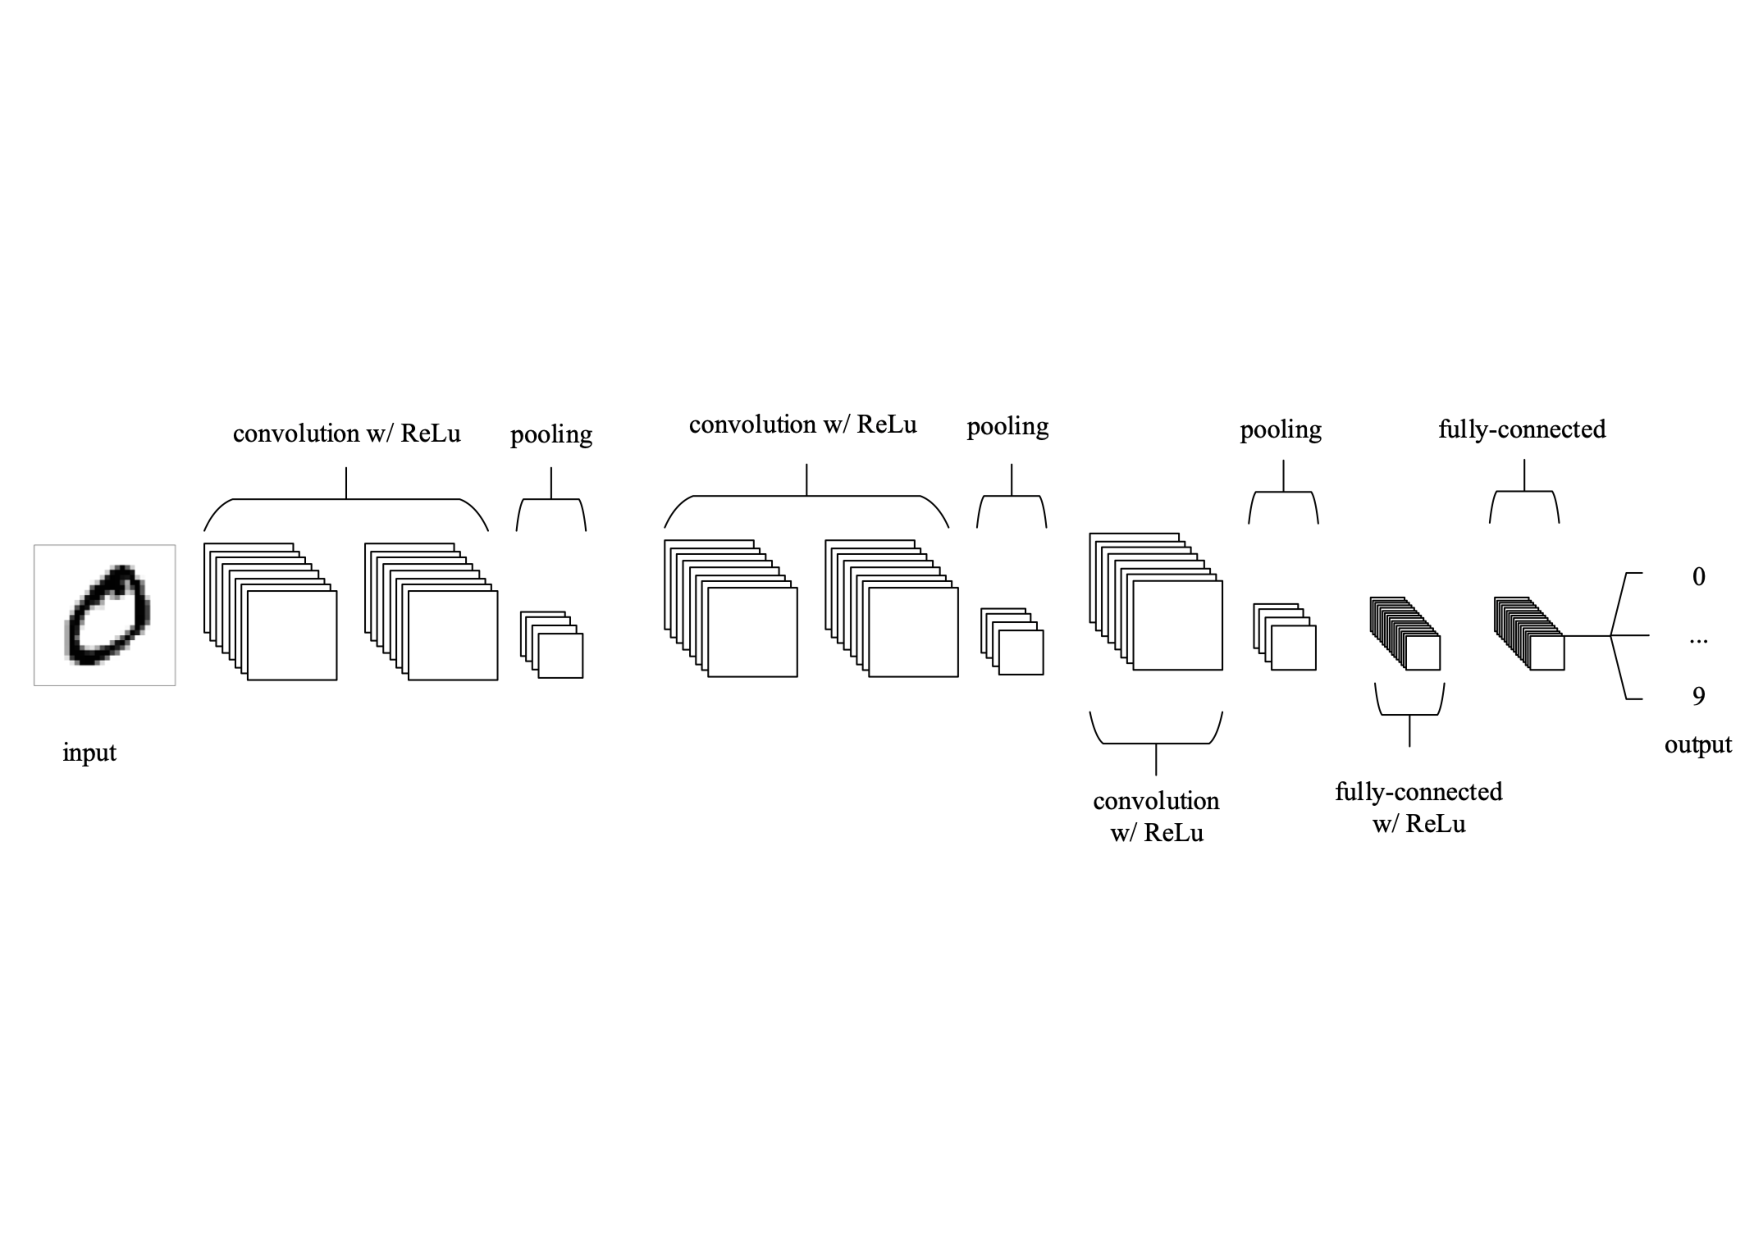
\includegraphics[width=0.9\textwidth]{cnn/cnn_architecture.pdf}
  \caption {Overview over CNN architecture \cite{OShea2015}}
  \label{fig:CNN_overview}
\end{figure}
Besides operations like Batch-Normalization, which are also common in regular neural networks, CNNs apply pooling layers. Pooling layers are responsible for downsampling the feature maps along the spatial dimensionality to reduce the complexity of the model. In the following typical CNN layers are described more in detail. 


\subsubsection{Kernels}
The convolutional layers are the core layers of a CNN. The learnable paramaters in a convolutional layer are the weights and biases of each kernel. During the optimization each kernel learns to extract expressive features. Usually the spartial dimensions (width, height) are reduced throughout the network in order to go from extracting global features in the beginning to more local features in the end. Since the kernels are applied at different regions of the input the kernel scans different locations for the learned features. The depth of a kernel is defined by the depth of the input. Each kernel produces a feature map of depth one. It is possible to apply several equal kernels such that the total depth of the feature map is increased. Each channel corresponds to the features extracted by one single kernel \cite{OShea2015}. Looking at fig. \label{fig:kernel_number} one can see how the kernel of depth 3 (orange) is applied on the input of depth 3 (blue). By using 128 kernels the resulting feature map is of depth 128.

\begin{figure}[htpb]
  \centering
  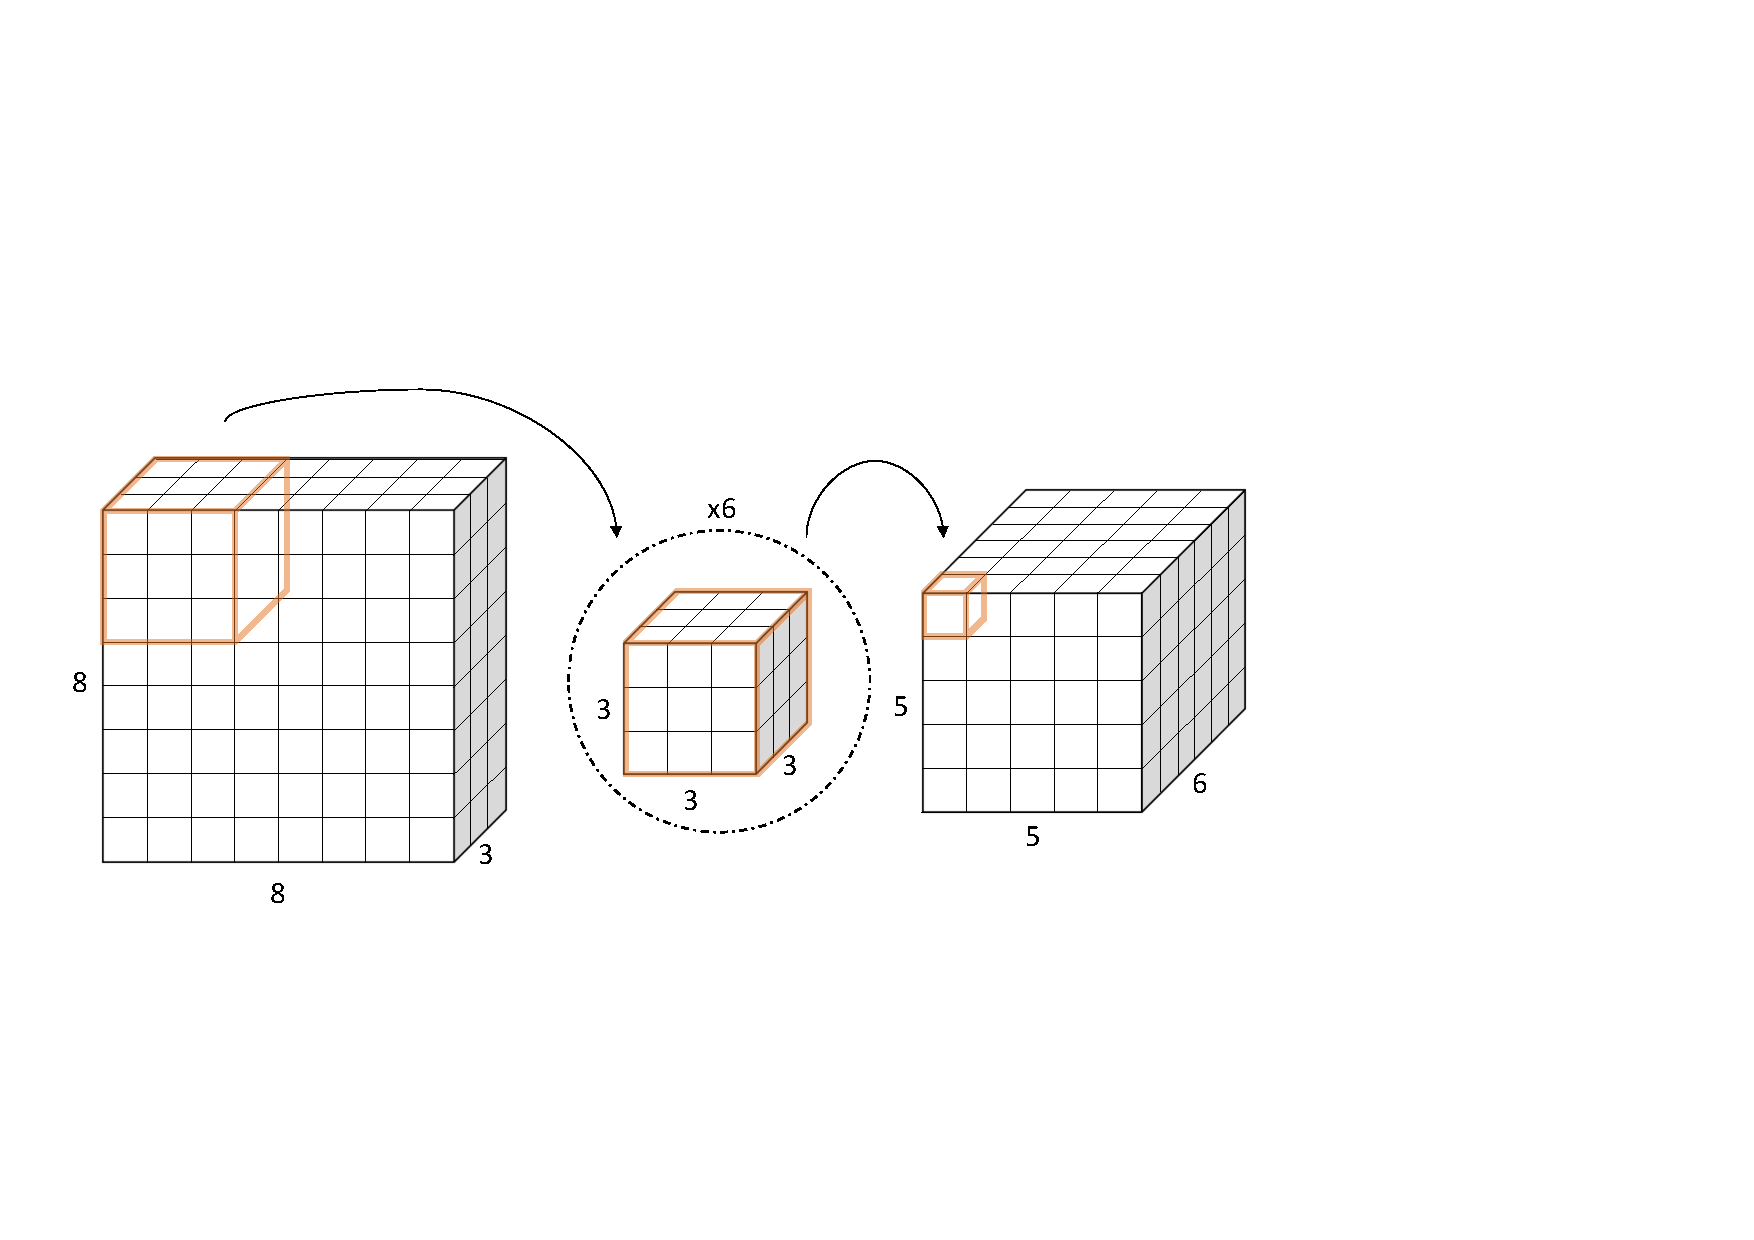
\includegraphics[width=0.6\textwidth]{cnn/kernel_number.pdf}
  \caption {2D convolution with 128 kernels of depth 3 \cite{Ganesh2019}}
  \label{fig:kernel_number}
\end{figure}
\FloatBarrier 

In a convolutional layer each kernel is convolved with the data across the whole spatial dimensionality. A feature map of new spatial dimension is created \cite{OShea2015}. To make things easier the convolution is shown for the 1D case:

\begin{equation}
  y(p_{0}) = \sum_{p_{n} \in R} w(p_{n}) \cdot x(p_{0} + p_{n}), 
  \label{eq:kernel}
\end{equation}

where $p_{n}$ is one of the $R$ cells in the kernel, $p_{0}$ is the starting pixel of the input. Each kernel cell is multiplied with the corresponding pixel in the input and the $R$ outputs are summed up in the pixel $p_{0}$ of the feature map \cite{Ganesh2019}. This process is also visualized in fig. \ref{fig:kernel}, where $p_{n}$ is one of the three cells within the kernel, $R$ is three in this case and $p_{0}$ marks the the position of the convolution in the input and feature map. In this case $p_{0}$ is two since the first pixel of the input is not used and the second pixel in the feature map is calculated.


\begin{figure}[htpb]
  \centering
  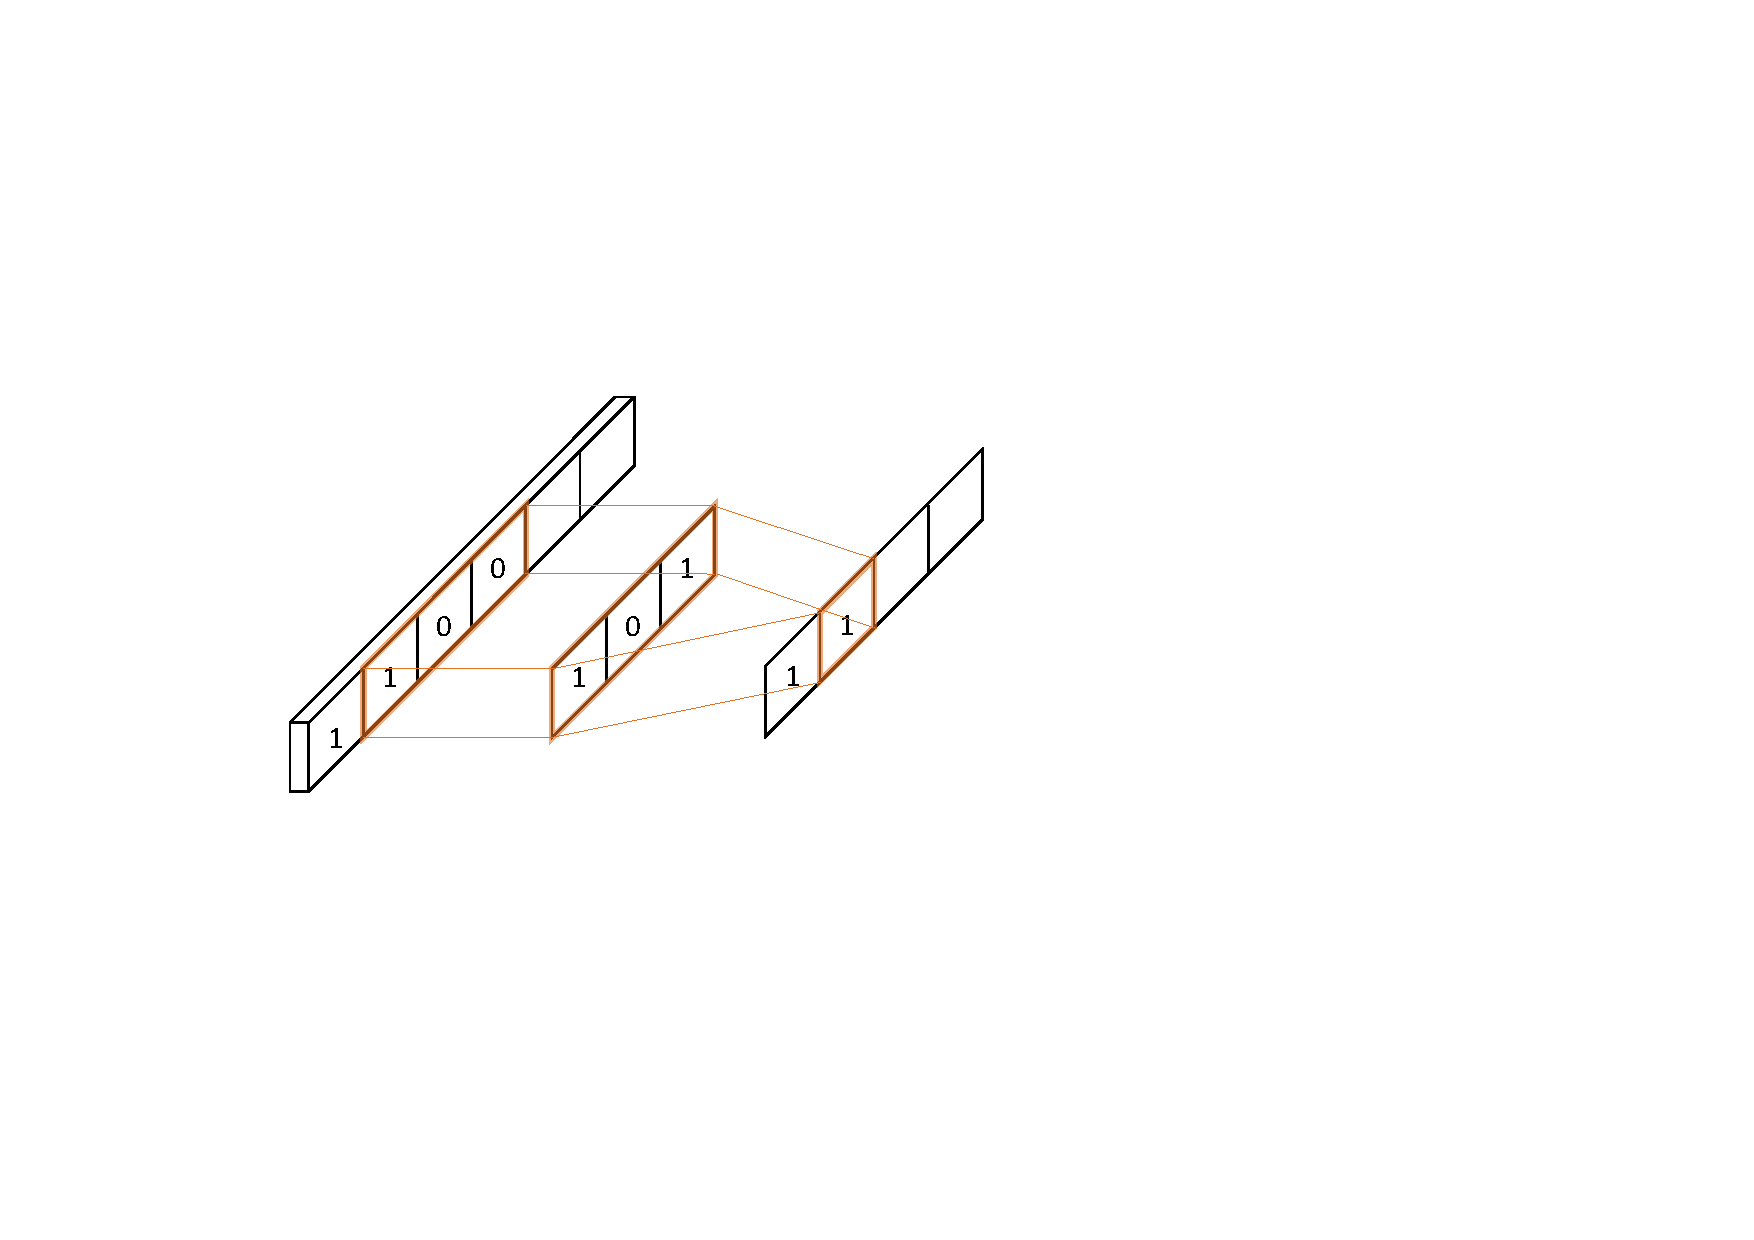
\includegraphics[width=0.5\textwidth]{cnn/kernel_calculation.pdf}
  \caption {Convolution of kernel an input \cite{Ganesh2019}}
  \label{fig:kernel}
\end{figure}

Compared to regular neural networks CNNs profit a lot from it's weight sharing concept. The kernel weights are learned throughout the training. Since the kernel is applied on different parts of the input, it is not necessary to train a weight for each input pixel. This reduces the number of learnable parameters in the network \cite{OShea2015}. Since the kernel is applied on different input locations, the feature search is insensitive to feature location in the image.

\subsubsection{Dilated convolution}

The dimensionality of the input which is processed by the kernel is called receptive field. When increasing the receptive field more global and otherwise more local features of the input are extracted. When defining a CNN architecture one has to find a trade-off between a model which is complex enough to capture the important information from the data and also keep the number of parameters low. Several hyperparameters can be used to reduce or increase the complexity of the model. After a convolutional layer three hyperparameters can be used to define the width and height of the resulting feature map. Dilated convolution, shwon in fig.\ref{fig:dilated_cnn}, is the same as regular convolution but it involves pixel skipping, so as to cover a larger area of the input. The kernel is not applied on a every neighbouring pixel \cite{Ganesh2019}.

\begin{figure}[htpb!]
  \centering
  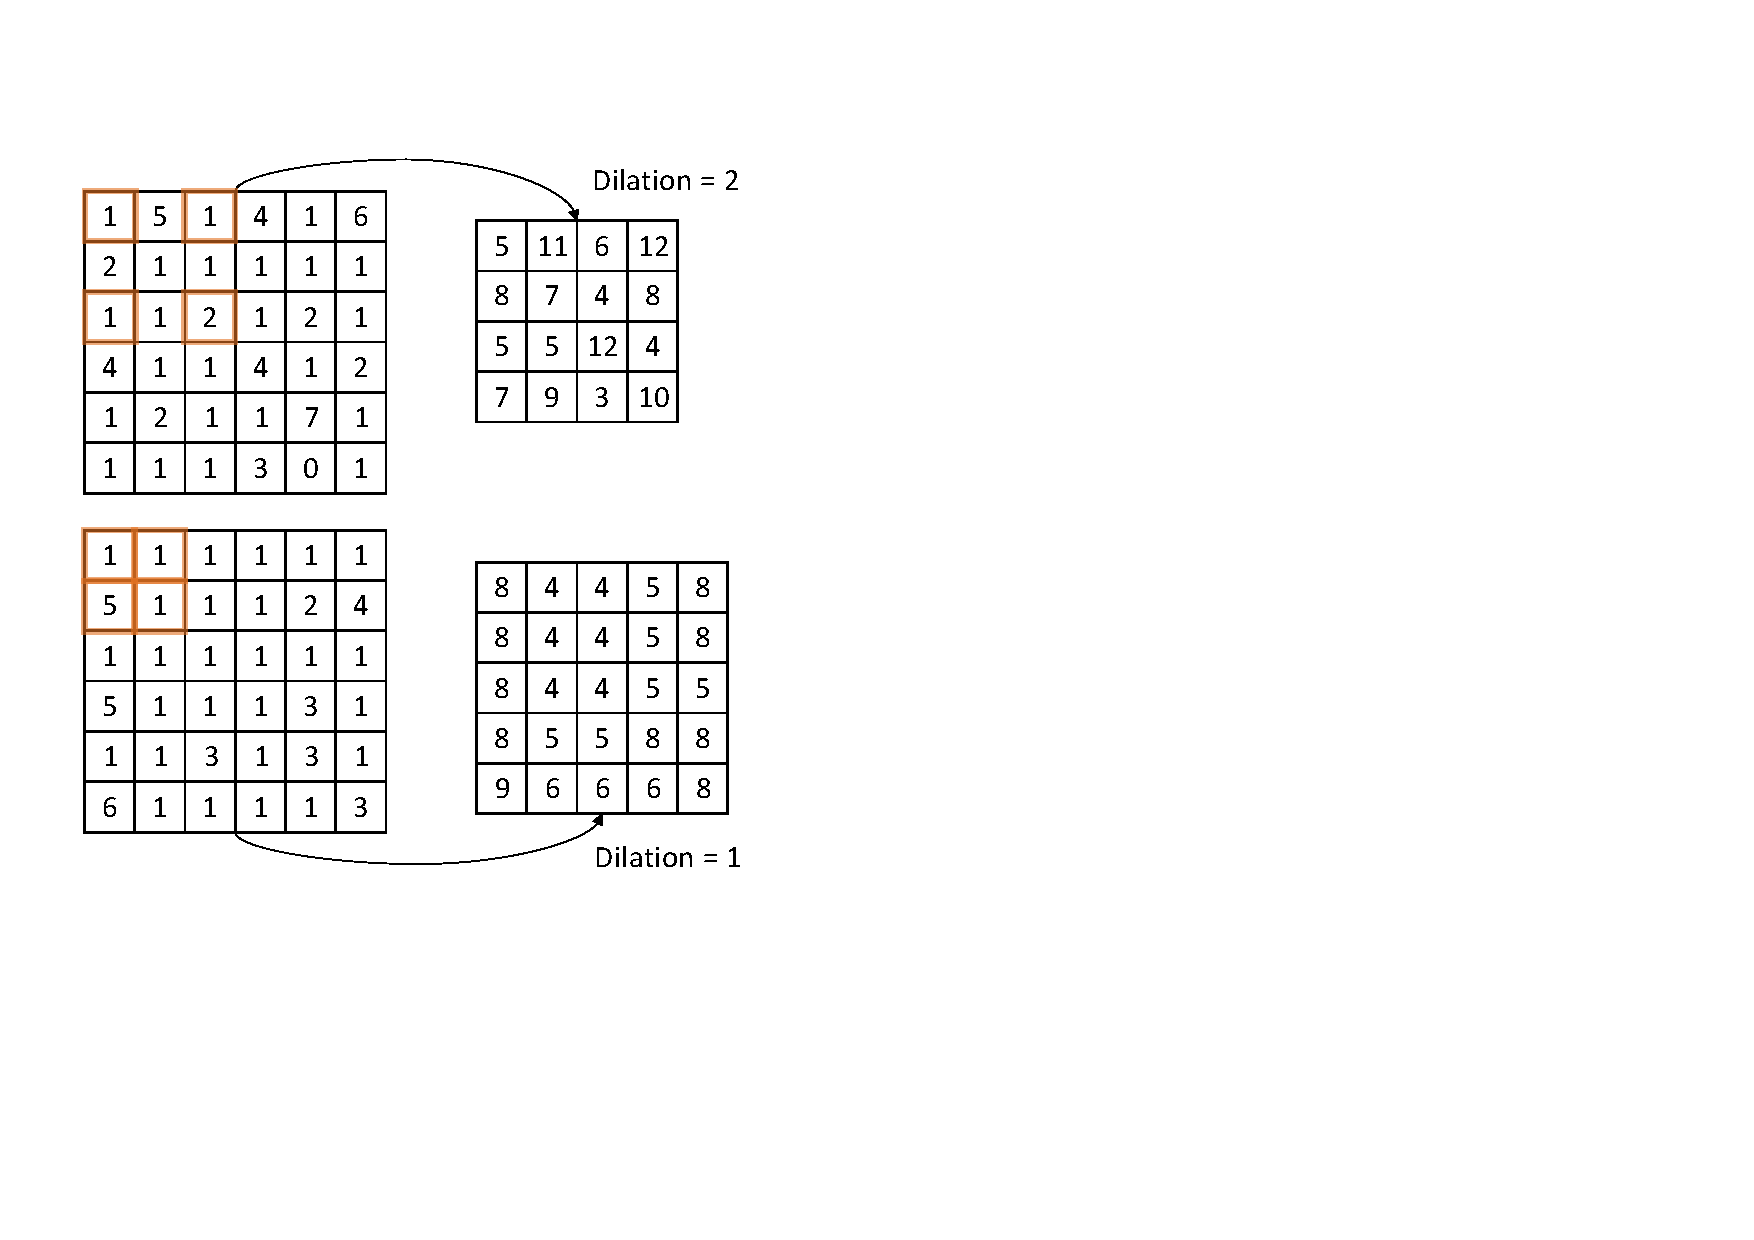
\includegraphics[width=0.5\textwidth]{cnn/dilation_cnn.pdf}
  \caption {Receptive field for convolution with different dilation factors}
  \label{fig:dilated_cnn}
\end{figure}
\FloatBarrier 

\subsubsection{Stride}
By increasing the stride the kernel skips several pixels while shifting over the input. The effects of an different stride factors are shown in fig.\ref{fig:stride_cnn}. The resulting feature map is decreased with an increased stride factor \cite{OShea2015}.

\begin{figure}[htpb]
  \centering
  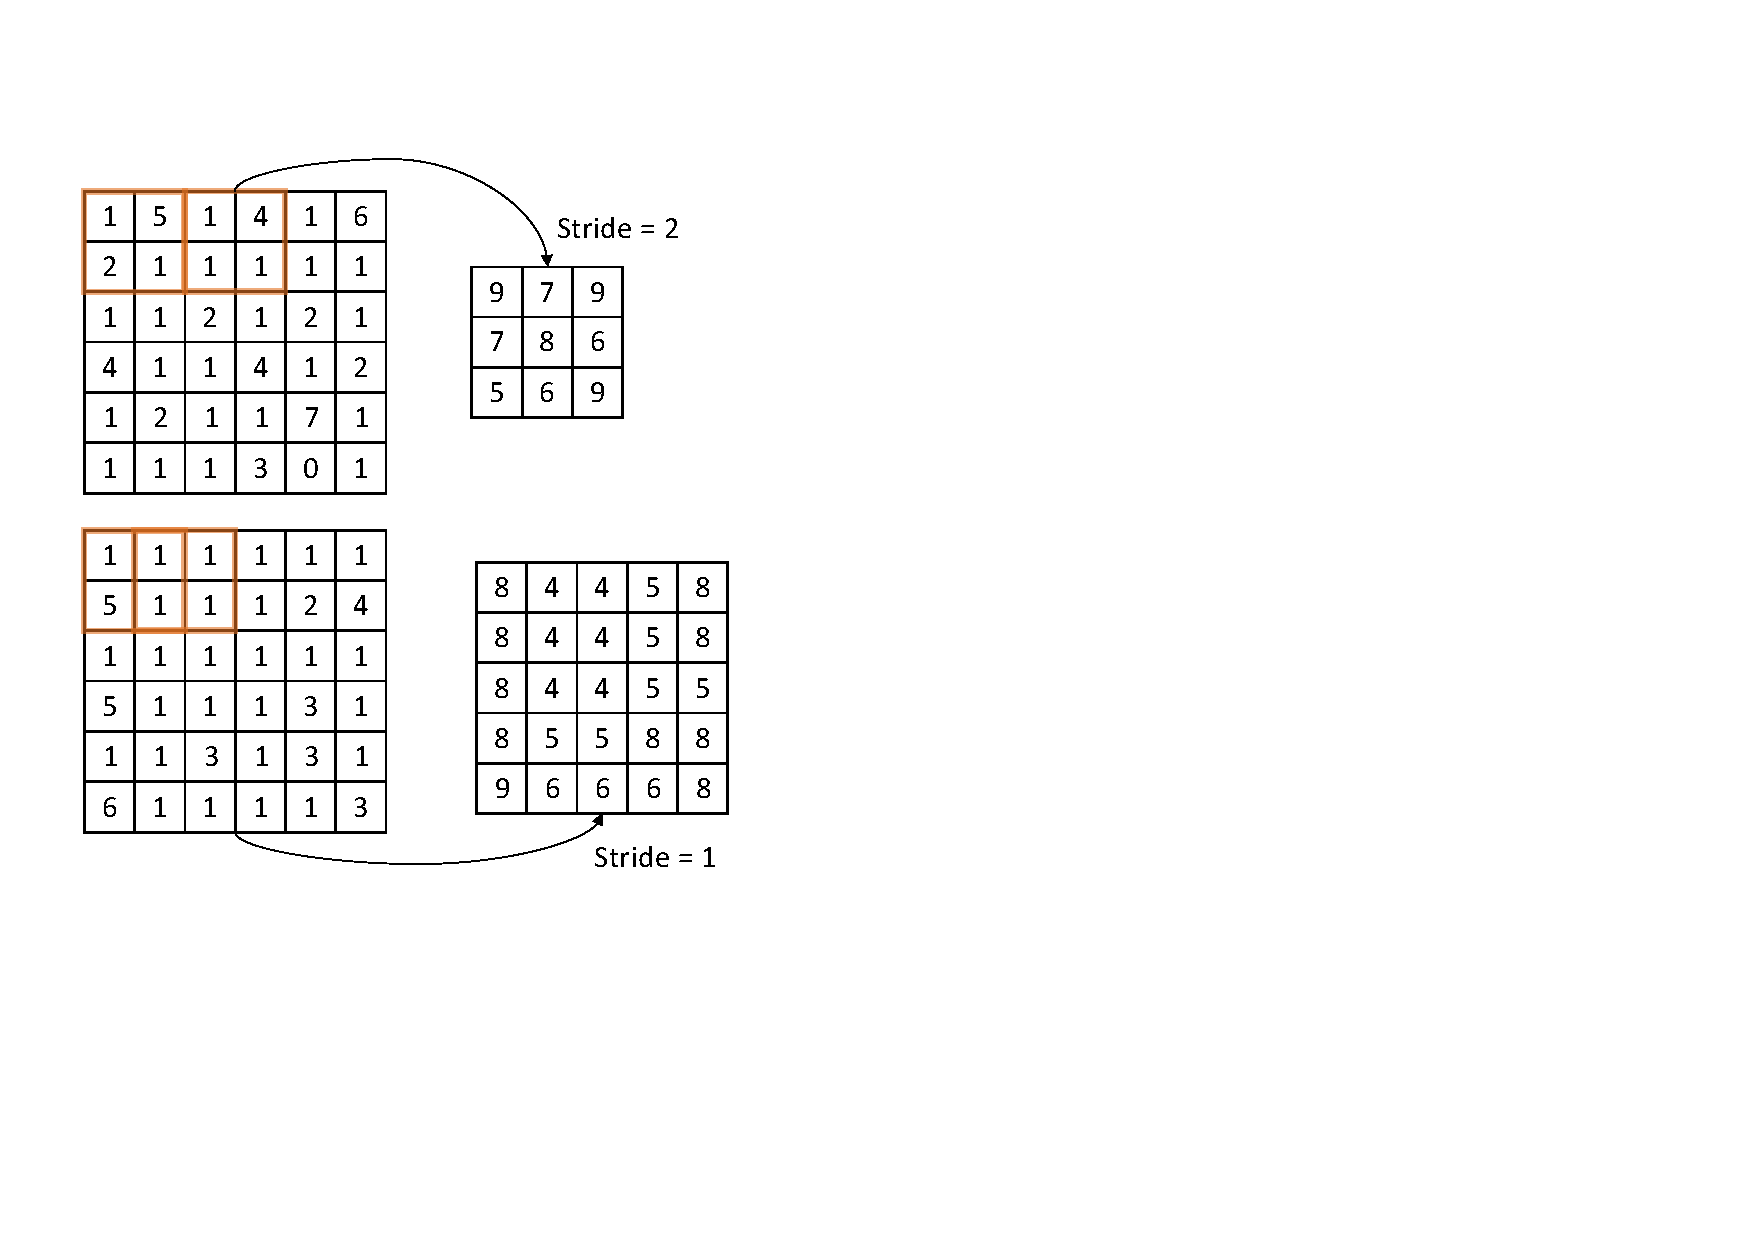
\includegraphics[width=0.5\textwidth]{cnn/stride_cnn.pdf}
  \caption {Convolution with different stride factors}
  \label{fig:stride_cnn}
\end{figure}
\FloatBarrier 

\subsubsection{Zero padding}
Zero padding, shown in fig.\ref{fig:zero_padding_cnn}, enlarges the input with a border of zeros, which increases the resulting feature map \cite{OShea2015}.

\begin{figure}[htpb]
  \centering
  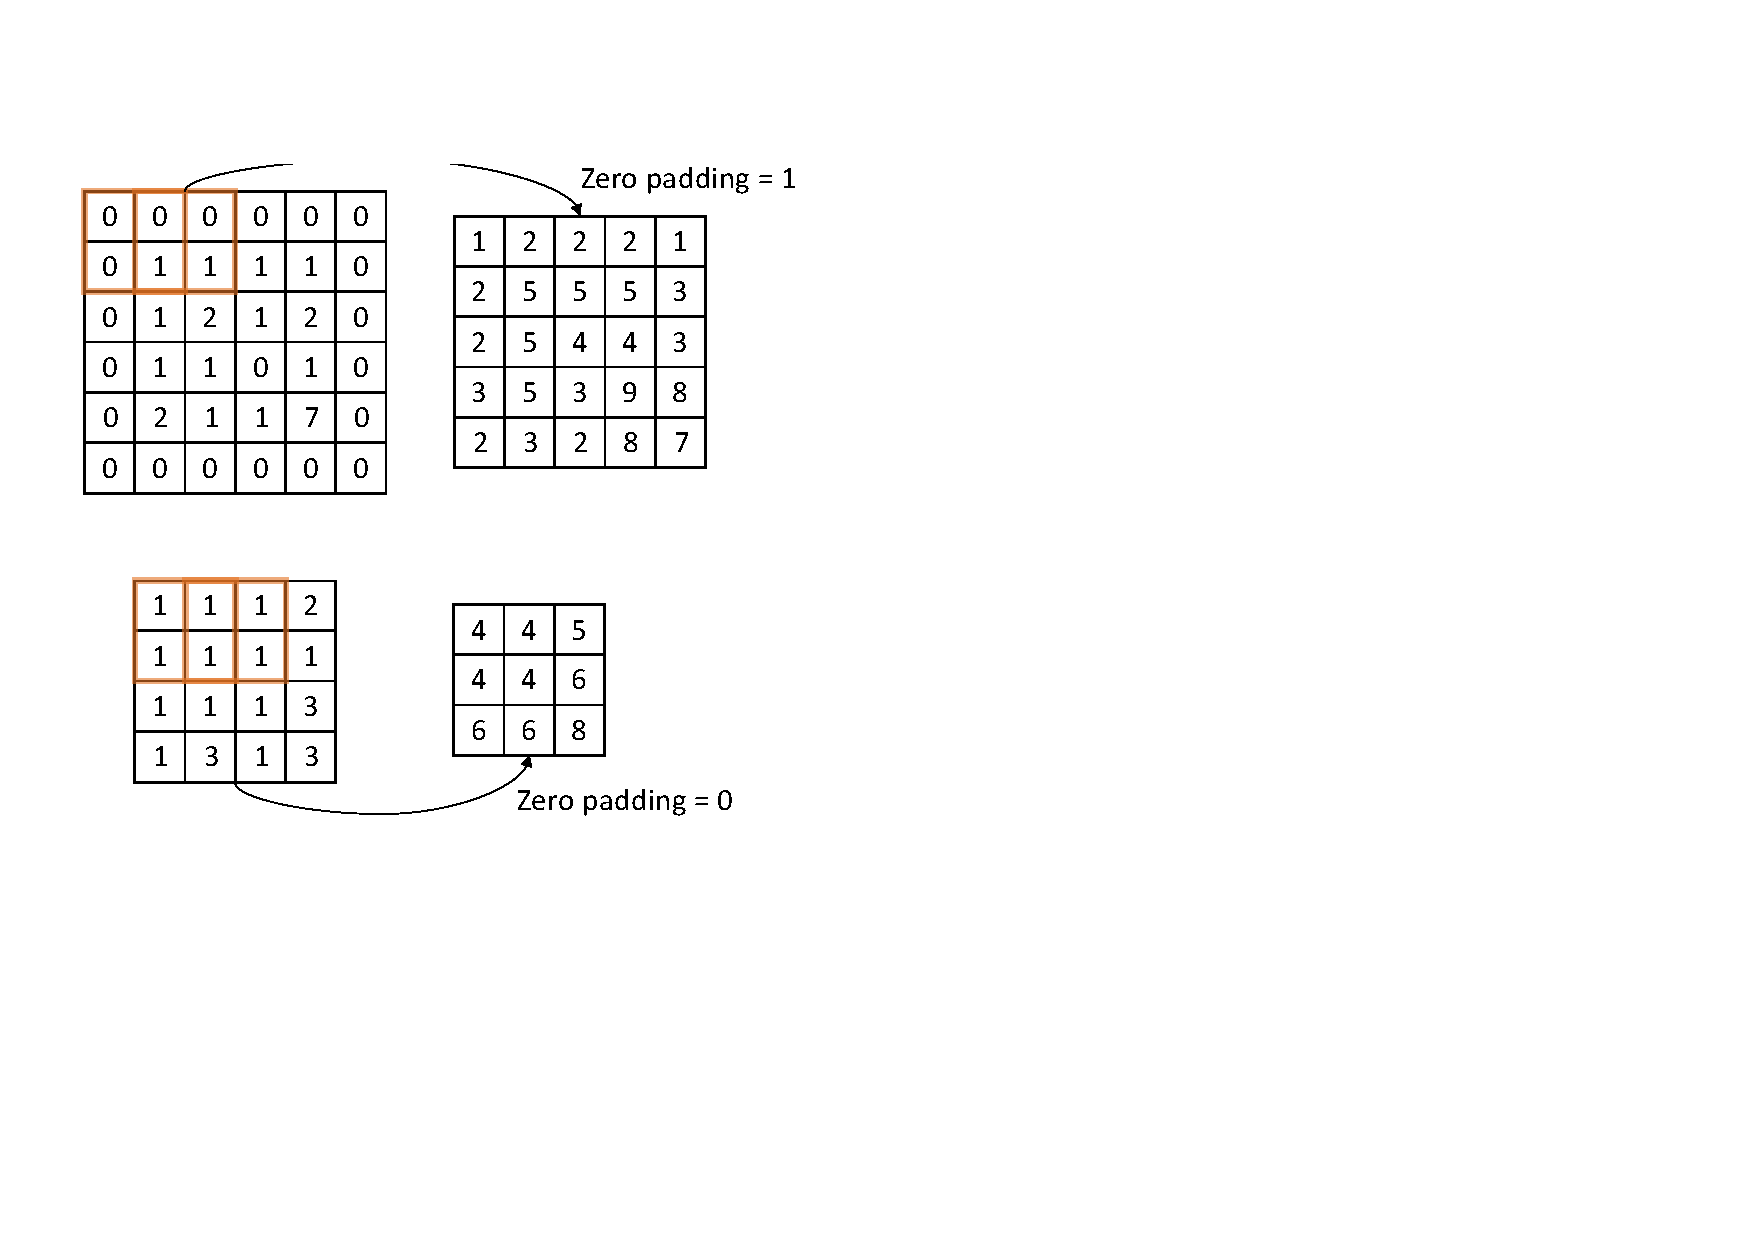
\includegraphics[width=0.5\textwidth]{cnn/zero_padding_cnn.pdf}
  \caption {Convolution with different zero padding}
  \label{fig:zero_padding_cnn}
\end{figure}
\FloatBarrier 


\subsubsection{Spatial dimensionality}

 The spatial dimensionality of the feature map right after a convolutional layer can be calculated as follows:

\begin{equation}
  \frac{(V-R)+2Z}{S+1}, 
  \label{eq:spatial_dimensionality_cnn_feature map}
\end{equation}
where V is the input size, R is the size of the receptive field, Z is the amount of zero padding and S refers to the stride.

\subsubsection{Pooling layer}
To change the spatial dimensionality of the data feed through the network one can also include pooling layers. There exist different variants like max-pooling and average pooling. In general these layers work identical as convolutional layers just that they do not have learnable parameters. Also pooling kernels are shifted over the input. For each kernel position all pixels covered by the kernel are merged to a single value. Max-pooling returns the maximal pixel value and average-pooling the average over all pixels. Often convolutional and pooling layers are applied consecutively \cite{OShea2015}.


\section{Domain adaptation and Transfer Learning}

In the computer vision community domain adaption and transfer-learning techniques recently received more and more attention. Knowledge learned from the supervised training data, denoted as source domain, is transferred to the unsupervised testing data, denoted as target domain. The target and source domain data come from different problems which must be related and structured similarly. Generally transfer learning approaches can be grouped in four different types. 

\begin{itemize}
\item \textbf{Instance-based transfer learning} where different weights are assigned to data samples from the source domain. These weights are proportional to the similarity between sample and target domain.
\item \textbf{Feature-based transfer learning} which has the goal to find a feature space in which the discrepancy between the domains is reduced.
\item \textbf{Model-based transfer learning} which uses classifiers that can be transfered directly or fine-tuned to make the model perform well on the target domain.
\item \textbf{Relation-based transfer learning} where the goal is to find and utilize similarities between the two domains to transfer knowledge \cite{AZAMFAR2020103932}. 
\end{itemize}

In order to compensate the domain shift problem in health monitoring tasks, domain adaption and transfer learning approaches are promising. Since the data from the source and target domain include the same machine health conditions and shared underlying features exist between them, domain adaptation approaches to compensate the domain shift are investigated. Fig.\ref{fig:Domain_adaption_intro} illustrates how feature-based domain adaption can be used to find a cross-domain classifier which accurately separates source and target domain data in a domain invariant feature space \cite{Pandhare2021}.

\begin{figure}[htpb]
  \centering
  \includegraphics[width=1\textwidth]{Domain_adaption_intro}
  \caption {Domain adaption for health monitoring of machines with different working conditions \cite{Pandhare2021}} \label{fig:Domain_adaption_intro}
\end{figure}






\section{Maximum Mean Discrepancy}
Maximum Mean Discrepancy (MMD) is a criterion which estimates the discrepancy between two distribution. MMD can be used to optimize the network such that the distribution discrepancy is reduced in a data domain-invariant feature space. The discrepancy is measured as squared distance between the distribution kernel embeddings in the reproducing kernel Hilbert space (RKHS). The distribution discrepancy across domains is measured in the layers of the neural network in order to avoid feature transferability degradation. One has to pay attention to not transfer noise or irrelevant information. This destroys the structure of the source and target domain data and therefore makes the classification task even more difficult \cite{li2020domain}. 

\begin{align}
    M_{k}(P,Q) = \Bigl|  \boldsymbol{E_{P}}[\Phi(\boldsymbol{X^{s}})] - \boldsymbol{E_{Q}}[\Phi(\boldsymbol{X^{t}})]     \Bigl|^{2}_{Hk}
\end{align}

Hk denotes the RKHS, which is described by the characteristic kernel k and the mapping function $\Phi$. Taking the identity function as mapping function results in matching the distribution means. When using more complex mapping functions also higher order moments can be matched \cite{Yujia2015}. The distributions of the source domain $X^{s} = \{{x}_{i}^{s}\}_{i=0,...,n_{s}}$ and target domain $X^{t} = \{{x}_{i}^{t}\}_{i=0,...,n_{t}}$ are represented by P and Q. $\boldsymbol{E_{p}[.]}$ is the expected value of the source distribution P in the feature space. The kernel choice is of great importance when applying MMD. For this reason it makes sense to combine several kernels in order to profit from their individual performance \cite{li2020domain}.

\begin{align}
    k(\boldsymbol{X^{s}}, \boldsymbol{X^{t}}) = \sum_{i=0}^{N_{k}} k_{\sigma_{i}}(\boldsymbol{X^{s}}, \boldsymbol{X^{t}})
\end{align}

$N_{k}$ denotes the number of kernels used in the the RKHS and $k_{\sigma_{i}}$ represents one individual RBF kernels. Also, other kernels like linear kernels could be used, but current research shows that RBF kernels usually perform best \cite{AZAMFAR2020103932}. In our attempt we used 5 RBF kernels with the bandwidth parameters 1, 2, 4, 8, 16.



% !TeX root = ../main.tex
% Add the above to each chapter to make compiling the PDF easier in some editors.

\chapter{Related Works}\label{chapter:related_works}


\section{Fault feature extraction for DL-based Predictive Maintenance}

Nonstationary signal analysis is one of the main topics in the field of machinery fault diagnosis. Nonstationarity in this sense means that the signals change their statistical properties over time. Signals can consist of multiple frequencies and change their amplitude while traveling in time. Traditional signal analysis techniques make stationary assumptions. When applying those just statistical average in time or frequency can be extracted \cite{FENG2013}. The demand for analysis methods, which allows ascertain features of such nonstationary signal is increasing. These features help to collect machine health related information from the signals.

Traditionally, Fourier transforms are an important tool in signal analysis. The Fourier transform relates the one-dimensional time- and frequency domains as following:

\begin{equation}
    \begin{aligned}
        & time-domain (signal): \\
        & x(t) = \int_{f} X(f) e^{j 2 \pi t f} df \\
        & frequency-domain (spectrum): \\
        & X(f) = \int_{t} x(t) e^{- j 2 \pi f t} dt, \\
    \end{aligned}
\end{equation}

Since both domains are not combined but just related, the time specific information are lost in the frequency domain and the other way around. The relation between the time- and frequency domain created by the Fourier transformation is visualized in fig. \ref{fig:fourier} 
\begin{figure}[p]
  \centering
  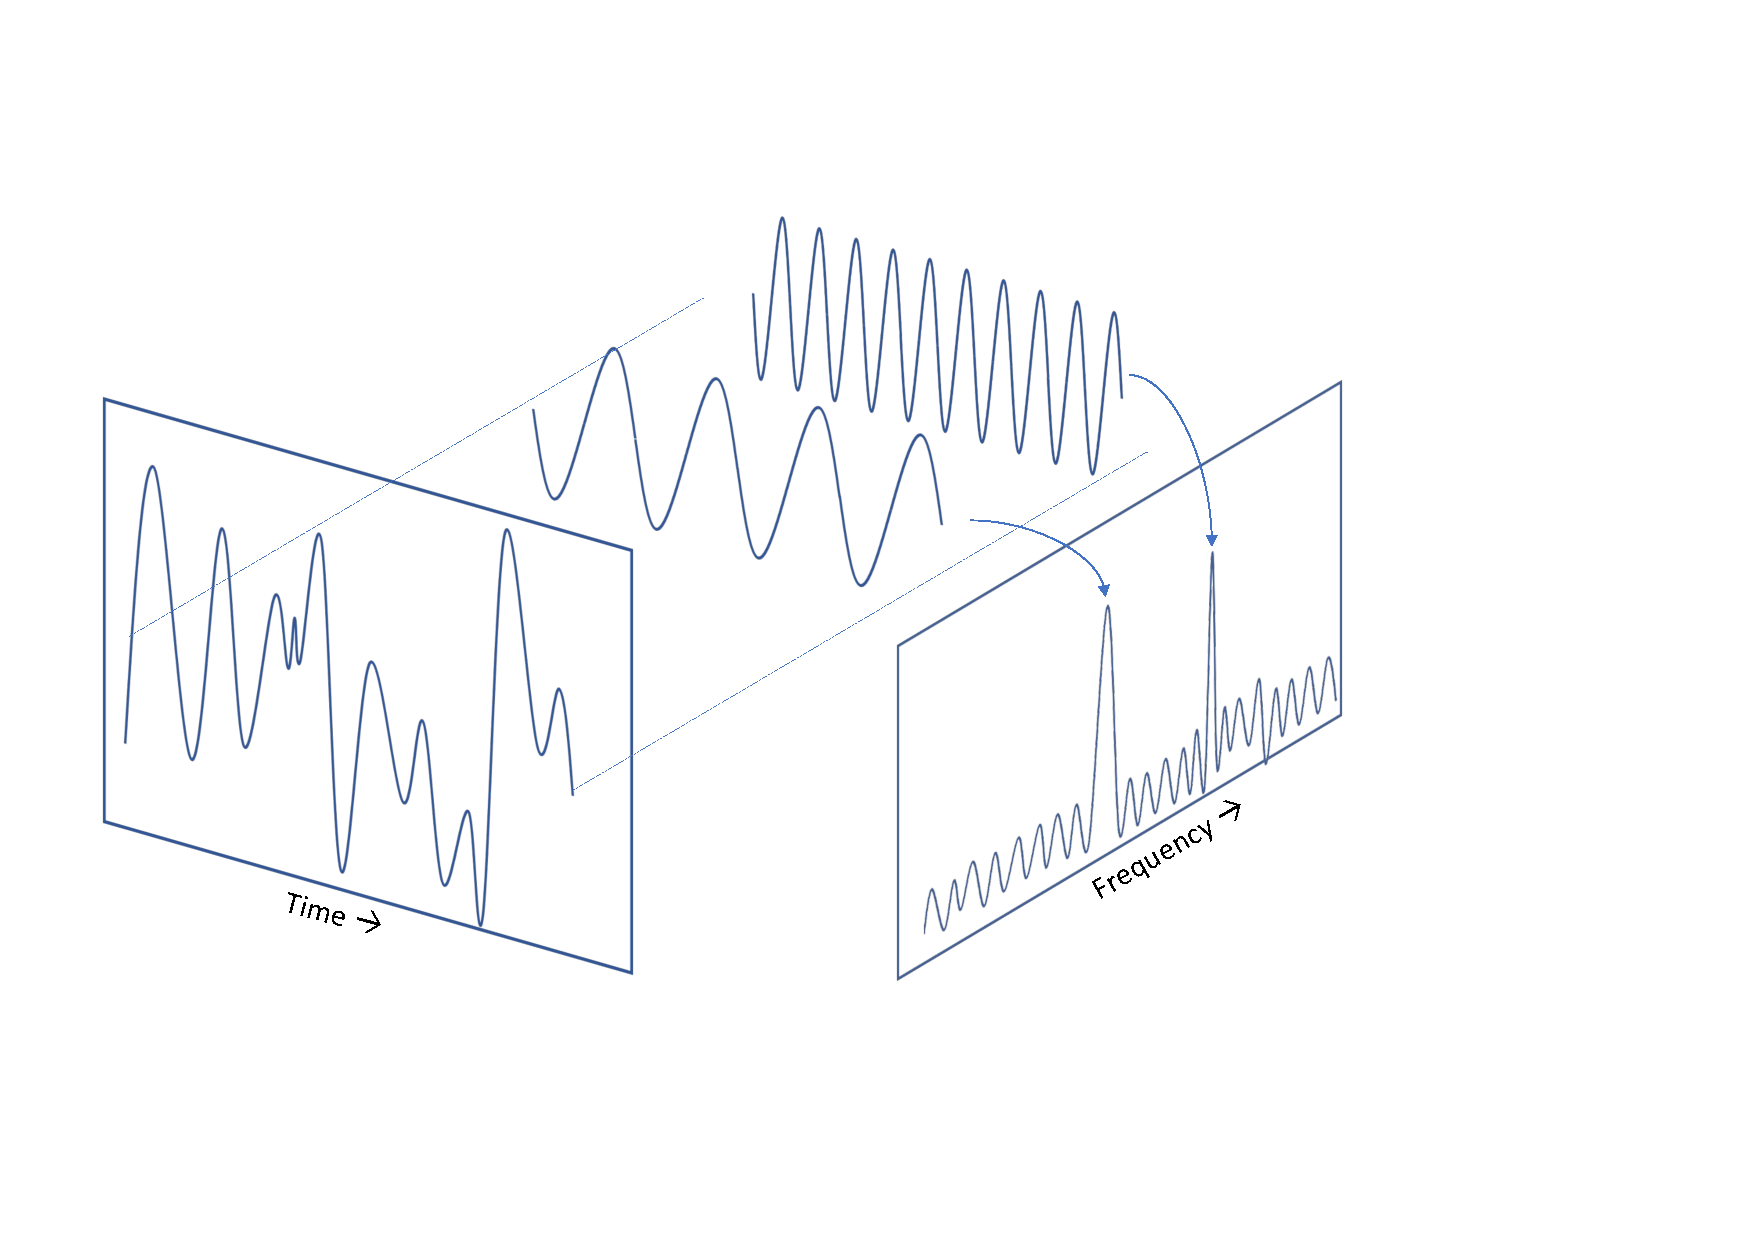
\includegraphics[width=.75\textwidth]{preprocessing_transform/fourier.pdf}
  \caption{Relation between time- and frequency domain through Fourier transformation}
  \label{fig:fourier}
\end{figure}

Time–frequency representations (TFR) solve this problem by transforming the one-dimensional signal in two-dimensional time-frequency plane, where each value corresponds to the dominance of a specific frequency at a certain point in time. Mathematically the two-dimensional data is represented by the joint function $T_{x}(f,t)$, where $x$ is the data of interest and the arguments of the function is the time  $t$ and frequency  $f$. One separates different methods of this type by the relation dependency of $T_{x}(f,t)$ on the input signal $x(t)$. There exit linear, quadratic or non-linear relationships.
The focus of this chapter is to describe linear and quadratic TFRs in more detail \cite{Hlawatsch1992}. 

\subsection{Linear time–frequency representations}
When the signal of interest can be decomposed in several linearly related components then the TFR of this signal can also be expressed as a linear combination of TFRs corresponding to each signal component:
\begin{equation}
    \begin{aligned}
        x(t) = c_{1} x_{1}(t) + c_{2} x_{2}(t) \rightarrow T_{x}(f,t) = c_{1} T_{x_{1}}(f,t) + c_{2} T_{x_{2}}(f,t)
    \end{aligned}
\end{equation}


All TFRs which fullfill this idea of linearity and superposition are called linear TFRs. The two most popular linear TFRs are the short-time Fourier and wavelet transform, which are presented in the following \cite{Hlawatsch1992}. 
\subsubsection{Short-time Fourier transform}

Short-time Fourier transform (STFT) is a method which adds a time variable to the traditional Fourier spectrum. This allows to investigate the variations in the signals spectrum over time. STFT assumes the signal's spectrum to be constant during a short time window. For each such window a Fourier spectrum is obtained and the time related changes are measured between such consecutive snapshots in the data. Window functions are defined which separate the signal. For each window a Fourier is applied. The process is mathematically expressed in the following:  
\begin{equation}
    STFT_{x}(t,f) = \int_{- \inf}^{+ \inf}x(\tau) w(\tau -t) exp(-j2\pi f \tau),
\end{equation}
where  $w(\tau -t)$ is the window function centered around t which is multiplied with the signal $x(t)$. Shifting the window over the signal and applying the Fourier transform $exp(-j2\pi f \tau)$ generates local spectra of the signal at for different points in time t \cite{FENG2013}. The time-frequency resolution is defined by the windowing function and the window length. STFT suffers from a trade-off between high resolution in time or in frequency but both at the same time is not possible. The optimum window length will depend on main interest behind the signal analysis. For accurate time domain information the window size needs to be reduced and for frequency domain information increased. STFT  decomposes the signal in existing sinusoidals and determines it's frequency and phase for a local part of the signal defined by the windowing function \cite{Hlawatsch1992}. 

\subsubsection{Wavelet transform}
The waveflet transform decomposes the signals in several wavelets which contain information about the health condition of the machine. A wavelet is a wave-like oscilation which is described by it's function, location and scale. The location defines where the wavelet overlaps with the signal and the scale defines how much squished (small scale) or streteched (big scale) the wavelet is. By changing the location of the wavelet it is shifted through the signal and overlaps with several different parts of the signal. While shifting the wavelet, it is multiplied with the signal  \cite{Shawhin2020}. The convolution of the wavelet and the signal is mathematically expressed in the following:
\begin{equation}
    WT_{x}(t,a) = \frac{1}{\sqrt{a}} \int_{- \inf}^{+ \inf} x(\tau) \psi(\frac{\tau -t}{a}) d \tau,
\end{equation}
 where $x(t)$ is the signal which is convolved with the wavelet $\psi(\frac{\tau -t}{a})$. In this case a is the scaling factor, t is the time shift and $frac{1}{\sqrt{a}}$ is a normalization factor to maintain the energy conservation \cite{FENG2013}. Different wavelet basis $\psi(t)$ can be convolved with the signal. This helps to analyze the signal for different pattern, which have similar properties as the wavelet \cite{Shawhin2020}. Possible wavelet basis could be the Gaussian, Morlet, Shannon, Meyer, Laplace, Hermit, or the Mexican Hat wavelets in both simple and complex functions \cite{Verstraete2017}. This allows a more extensive, flexible and detailed analysis. In fig. \ref{fig:ricker_wavelet} Ricker wavelets with different scales are visualized. Besides that wavelet transforms can extract local spectral and temporal information in parallel \cite{Shawhin2020}.


\begin{figure}[p]
  \centering
  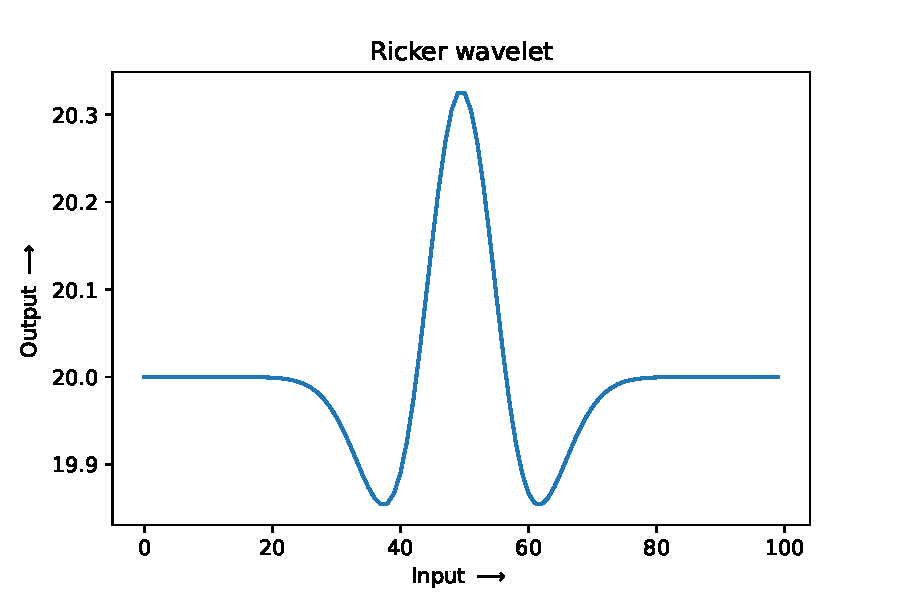
\includegraphics[width=.47\textwidth]{preprocessing_transform/wavelet_small_scale.pdf}
  \hspace{.1cm}
  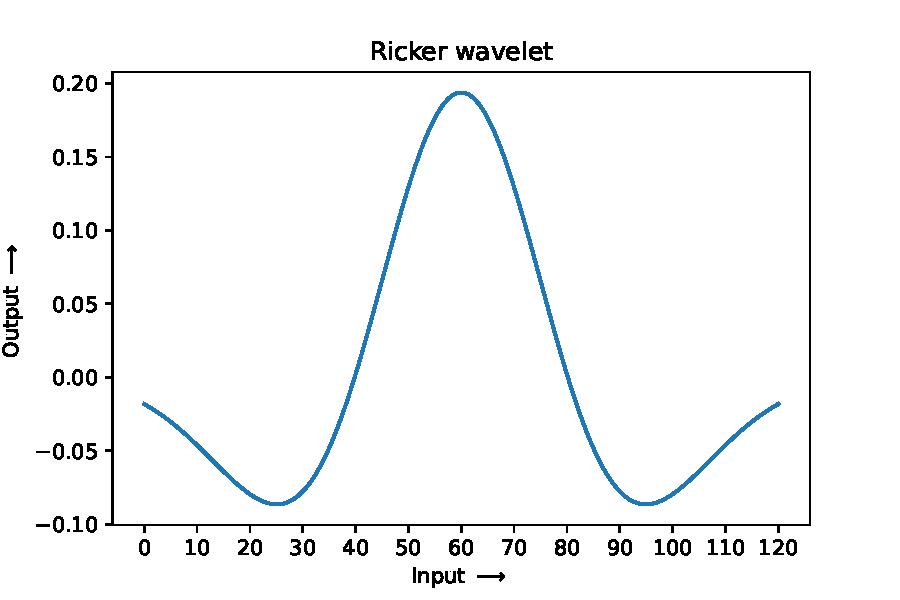
\includegraphics[width=.47\textwidth]{preprocessing_transform/wavelet_big_scale.pdf}
  
  \vspace{.1cm}
  
  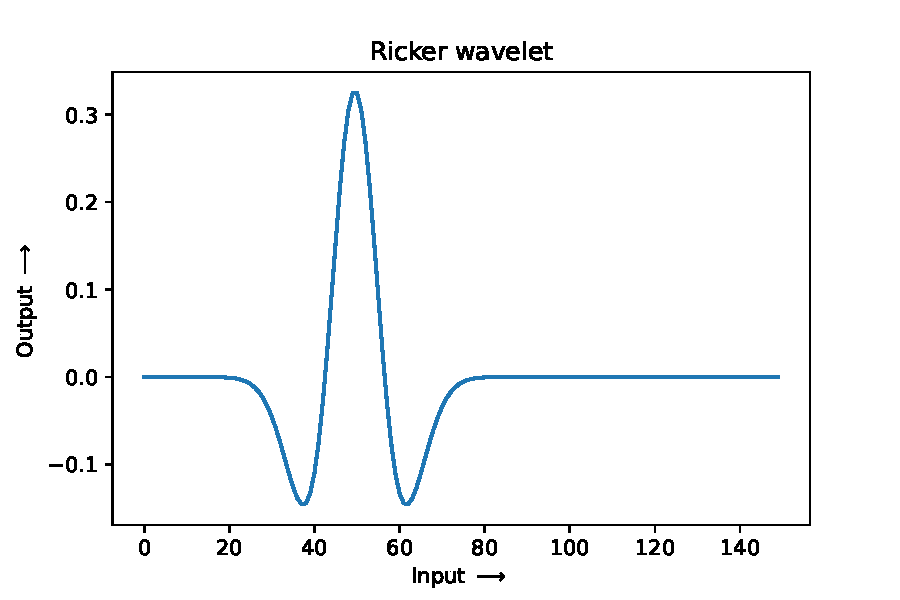
\includegraphics[width=.47\textwidth]{preprocessing_transform/wavelet_left_scale.pdf}
  \hspace{.1cm}
  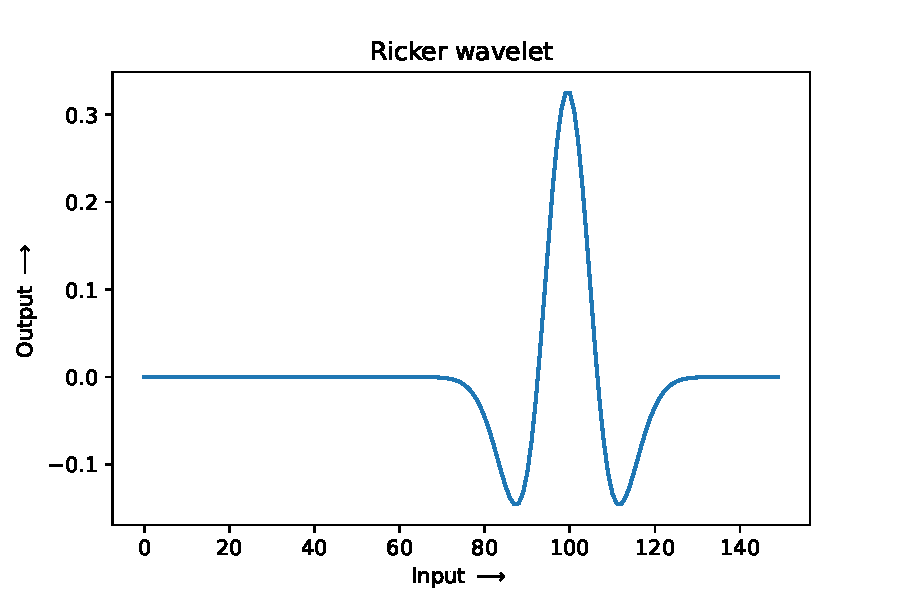
\includegraphics[width=.47\textwidth]{preprocessing_transform/wavelet_right_scale.pdf}

  \caption{Ricker wavelet with different scale (top) and shifting (bottom) factors}
  \label{fig:ricker_wavelet}
\end{figure}
\FloatBarrier 

\subsection{Spectrograms and Scalograms}

 Spectrograms are a graphic representation of the STFT and scalograms of the wavelet transform. Spectrograms and scalograms visualize the the squared magnitudes of the previously presented STFT and Wavelet transform. This squared magnitude are loosly interpreted as as signal energy \cite{Hlawatsch1992}. The mathematical expressions are presented in the following: 

\begin{equation}
    \begin{aligned}
        &SPEC_{x}(t,f) = \abs{STFT_{x}(t,f)}^{2} \\
        &SCAL_{x}(t,f) = \abs{WT{x}(t,f)}^{2}, 
    \end{aligned}
\end{equation}

where $STFT_{x}(t,f)$ is the Short-time Fourier transform, $WT_{x}(t,f)$ the wavelet transform, $SPEC_{x}(t,f)$ the spectrogram and $SCAL_{x}(t,f)$ the scalogram \cite{Hlawatsch1992}. This way of representing the system energy in the 2d time and frequency space may reveal useful information from the complex and high-dimensional data without the need for additional feature extraction. As described before spectrograms have a fixed frequency resolution that is defined by the windows size. Scalograms on the other hand have a frequency- dependent frequency resolution \cite{Verstraete2017}.

\subsection{Adaptive non-parametric time–frequency analysis}
Adaptive non-parametric approaches include empirical mode decomposition (EMD) \cite{FENG2013}. Unlike other multiresolution analysis (MRA) techniques such as wavelet analysis EMD recursively extracts Intrinsic Mode Functions (IMF) from a non-stationary time series. According to Faltermeier et al. \cite{Faltermeier2010} IMFs have the following properties: 

\begin{itemize}
    \item [1] An IMF has just one extremum between to zero crossings. Local minima and maxima do need to alternate such that the number of local minima and maxima does differ at most by one. 
    \item[2] An IMF need to have zero mean, but still the IMF can have changing frequencies and amplitude modulation. 
\end{itemize}

The EMD algorithm decomposes the signal as following:

\begin{equation}
    x(t) = \sum_{n} x_{n}(t) + r(t),
\end{equation}
where $x(t)$ is the signal, $x_{n}(t)$ the n-th IMF and $r(t)$ the residuum \cite{Faltermeier2010}. Faltermeier et al. \cite{Faltermeier2010} describte the recursive extraction of IMFs from the signal as following: 
\begin{itemize}
    \item [Step 0:] Initialize: $n := 1$, $r_{0}(t) = x(t)$
    \item [Step 1:] Extract the n-th IMF as follows:
    \begin{itemize}
         \item [a)] Set $h_{0}(t) := r_{n−1}(t)$ and $k := 1$
         \item [b)] Find all local maxima and minima of $h_{k−1}(t)$
         \item [c)] Construct envelopes for all the identified maxima $U_{k−1}(t)$and minima $L_{k−1}(t)$ for $h_{k−1}(t)$ using cubic interpolation
         \item [d)] Determine the mean $m_{k−1}(t) = 12 (U_{k−1}(t) - L_{k−1}(t))$ of both envelopes of $h_{k−1}(t)$.
         \item [c)] Form the k − th component $h_{k}(t) := h_{k−1}(t) - m_{k−1}(t)$
         \begin{itemize}
            \item [i)] if $h_{k}(t)$ is not in accord with all IMF criteria, increase $k \rightarrow k + 1$ and repeat starting at step b
            \item [ii)] if $h_{k}(t)$ satisfies the IMF criteria then set $x_{n}(t) := h_{k}(t)$ and $r_{n}(t) := r_{n-1}(t) − x_{n}(t)$
         \end{itemize}
    \end{itemize}
    \item [Step 2:] Check another IMF needs to be extracted
        \begin{itemize}
            \item [i)] if $r_{n}(t)$ is the residue, the original data is decomposed in the n IMFs  $x_{n}(t)$ and the residue $r_{n}(t)$
            \item [ii)] if $r_{n}(t)$ is not the residue, go to Step 1.
         \end{itemize}
\end{itemize}


The number of IMFs extracted roughly equls $log_{2}(N)$ where $N$ is the number of extrema in the signal. The EMD decomposes the non-stationary signal in its locally and non-overlapping component IMFs. This process does not need any predefined wave-forms like the wavelet transformations expects it. The selection of the IMFs is an automatic and adaptive time-variant filtering  \cite{Faltermeier2010}. Compared to the Fourier and Wavelet transform, the the decomposition of the signal in several IMFS does not divide the signal into fixed frequency components, which gives HHT a higher time-frequency resolution \cite{Verstraete2017}. The popular Hilbert-Huang Transform (HHT) combines the EMD with the Hilbert spectral analysis. For this each the Hilbert transform is applied to each of the detected IMFs. A corresponding analytical signal can be constructed. Also the Hilbert amplitude and energy spectrum can be derived. For more Hilbert-specific details Feng et al. \cite{FENG2013} can be studied.


\section{Domain adaptation approaches for Predictive Maintenance}
In recent years, intelligent data-driven machine condition monitoring systems have replaced traditional approaches to a great extent. When using such monitoring systems for long time horizons operational conditions and therefore fault characteristics might change. This leads to unsatisfactory diagnosis performance \cite{AZAMFAR2020103932}. Furthermore, there are scenarios where not all fault classes are known during training. Due to the unexpected nature of faults, and the correlation and dependency between different parts of the system, faults can have numerous causes and can influence the systems in different ways. Therefore it is unlikely that the data used for training the model includes all system states and fault scenarios. Monitoring systems which can handle unseen classes and expand its knowledge adequately during test time seems helpful for industrial fault diagnosis systems \cite{Michau2017}. In order to address those issues domain adaption approaches seem promising in the area of fault diagnosis. In the literature deep-learning based domain-adaption is a hot topic. With its origin in the computer vision community it also made its way into the area of predictive maintenance, which will be discussed in the following. 

\subsection{Deep distance metric learning}
A domain adaption algorithm which optimizes the inter- and intra-class distance in the latent feature space and reduces the domain discrepancy with an MMD loss was presented by Li et al \cite{Li2018}. As visualized in fig. \ref{fig:Deep_distance_metric_learning_model} the model proposed by Li et al contains a CNN with a consecutive classifier. In a preprocessing step the raw vibration signal is first transformed in the frequency domain by applying wavelet transforms. Max-Pooling layers are included in order to reduce the data dimensionality. Batch-normalization layers are included to reduce the internal-covariate-shift by normalizing the input distributions of the hidden layers to the desired Gaussian distribution. As a regularization method dropout layers with a rate of 0.5 are included to avoid overfitting. 

\begin{figure}[p]
  \centering
  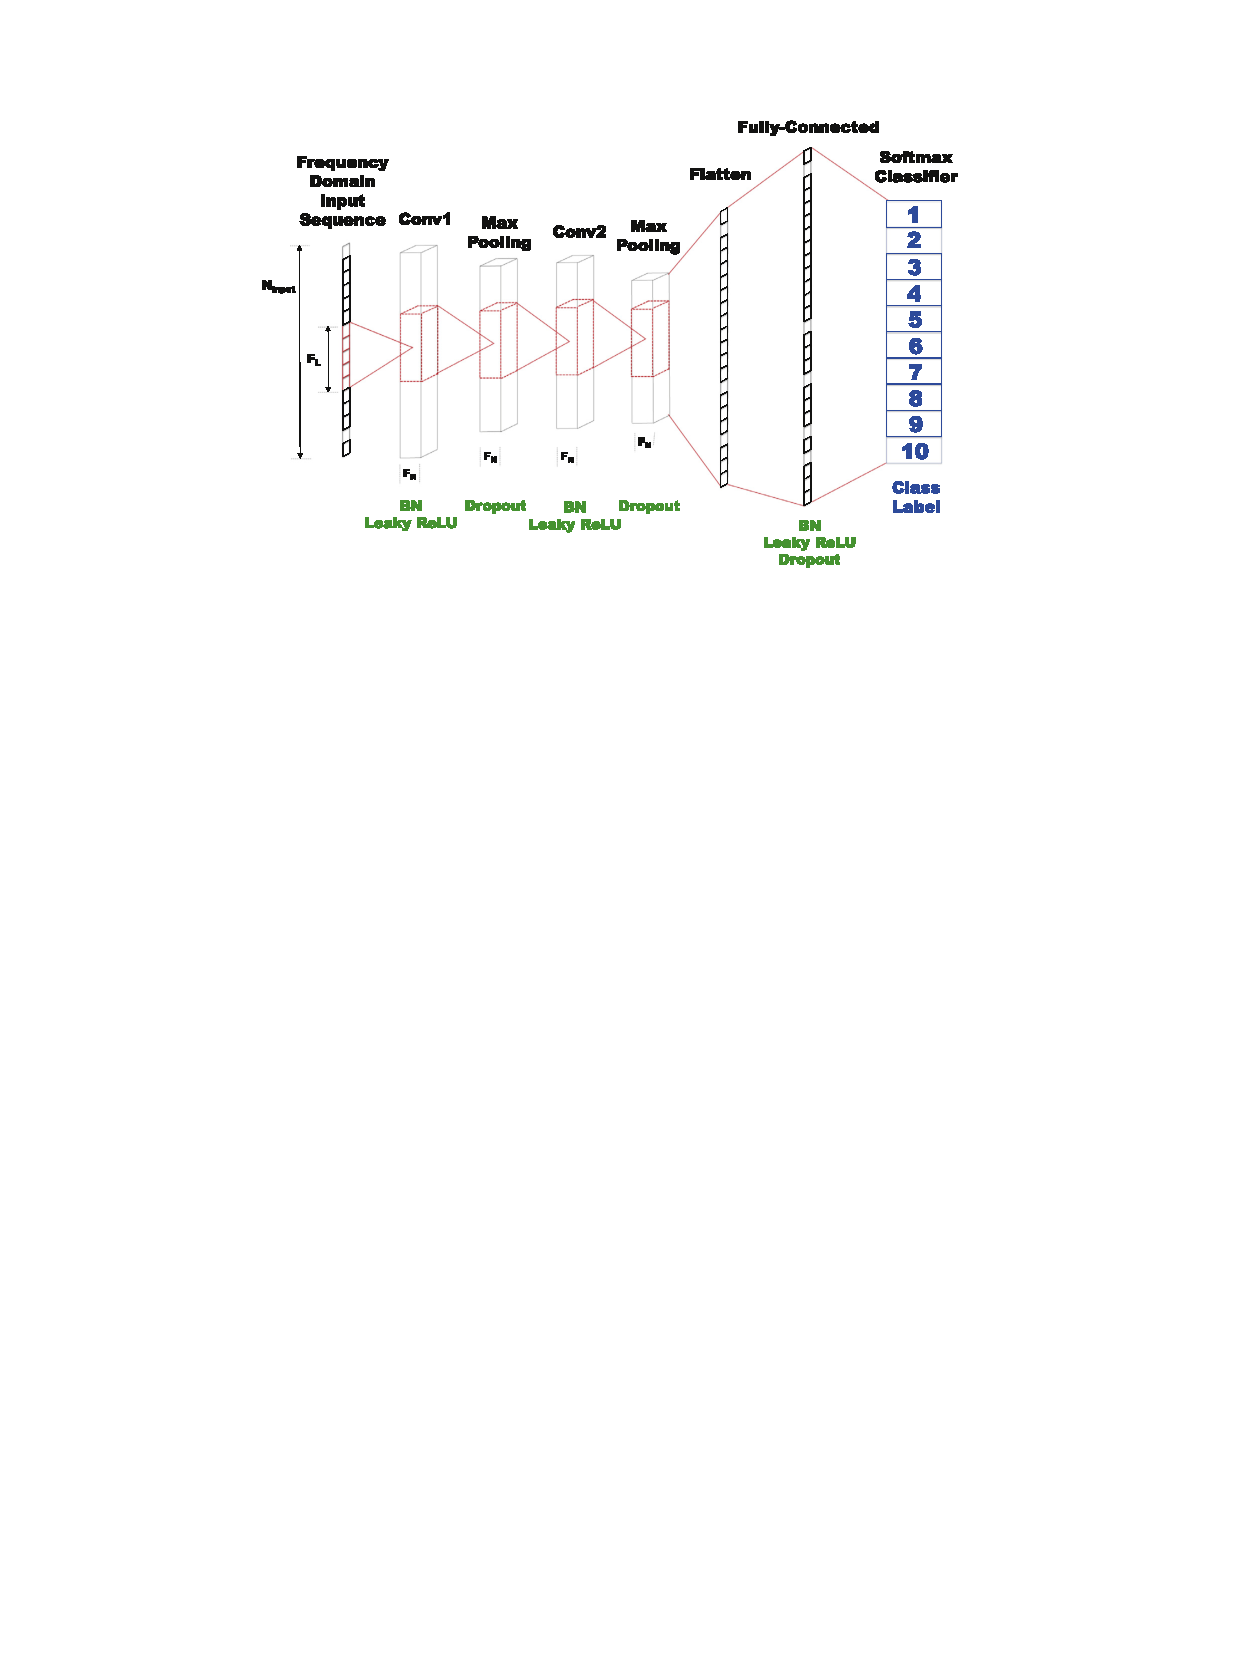
\includegraphics[width=.75\textwidth]{models_state_of_the_art/Deep_distance_metric_learning_model.pdf}
  \caption{Deep distance metric learning model \cite{Li2018}}
  \label{fig:Deep_distance_metric_learning_model}
\end{figure}

Li et al suggest to optimize the model such that the distance between samples of the same class is minimized and that between samples of different classes is maximized. This increases the separability between samples of different classes and the the compactness of samples belonging to the same class, which makes the algorithm more robust against environmental noises. In order to calculate the intra- and inter-class distance the expectation and variance of the samples of one class in the source dataset is measured. The distances can be measured as following:

\begin{equation}
    \begin{aligned}
       &D_{inter} = |E[f^{(m)}x^{(i)}]-E[f^{(m)}x^{(j)}]|_{2}-\sqrt{Var[f^{(m)}x^{(i)}]}-\sqrt{Var[f^{(m)}x^{(j)}]}\\
       &D_{intra} = 
        \sum_{i=1}^{N_{class}} \sqrt{Var[x^{(i)}]},
    \end{aligned}
\end{equation}

where $x^{(k)}$ denote the raw input sample of class k, $N_{class}$ is the number of the classes, $f^{(m)}x^{(k)}$ denotes the output at the m-th layer in the network and $E[f^{(m)}x^{(i)}]$ and $Var[x^{(i)}]$ are the  expectation and variance of of the samples belonging to class k in the mth layer. Optimizing the network with $J_{Cluster} = - D_{inter} + \eta D_{inter}$ reduces the inter- and maximizes the intra-class distance. Since $J_{Cluster}$  requires labels for each sample the optimization is restricted to the source domain data. Furthermore, Li et al applies a MMD loss to reduce the discrepancy between target and source domain: 

\begin{equation}
    \begin{aligned}
    J_{MMD,m} = MMD_{k}(P^{f(m}, Q^{f(m}),
    \end{aligned}
\end{equation}

where $P^{f(m}$ and $Q^{f(m}$ denote the representation of source and target samples in the mth hidden layer. Lastly, a cross entropy loss in the final layer optimzies the network to classify the source samples correctly. In total the network is optimized with the following weighted average of losses: 

\begin{equation}
    \begin{aligned}
    J_{total} = \alpha J_{Cluster} + \beta J_{MMD} + \gamma J_{CE}, 
    \end{aligned}
\end{equation}
where $J_{Cluster}$ is the cluster loss, $J_{MMD}$ the MMD loss,  $J_{CE}$ the cross entropy loss and $\alpha$, $\beta$ and $\gamma$ are the weights for calculating the weighted average \cite{Li2018}.


\subsection{Deep convolutional transfer learning network (DCTLN)}
Predictive maintenance of rolling bearing is a popular problem in the industry. Guo et al \cite{Guo2019} propose a health condition classifier which reduces the domain discrepancy by applying a MMD loss and using a domain classifier. The architecture of the model is visualized in fig. \ref{fig:DCTLN_model}. Features are extracted by a CNN containing 16 layers including one input layer, six convolutional layers, six pooling layers, two fully connected layers, and one output layer. Each convolutional layer is combined with a consecutive pooling layer.


The model is optimized with a combination of three losses
\begin{itemize}
    \item [1.] Reducing the health condition classification loss on the source domain data
    \item [2.] Maximize the Domain classifiaction loss on the source and target domain data 
    \item [3.] Minimize the MMD distance between the source and target domain data in the FC2 layer
\end{itemize}

\textbf{Objective 1}: By applying the cross entropy loss the model minimizes the health condition classification error on the source domain data.

\textbf{Objective 2}: The domain classifier processes the features in the hidden layer FC3 in order to predict the corresponnding domain of each sample. If the model is able to extract domain independent features the error of the domain classifier is increased.

\textbf{Objective 3}: The domain discrepancy is reduced by applying the MMD loss to the features in the hidden layer FC2. By applying the MMD loss the model reduces the distance between different domains in the FC2 feature space. More domain invariant featrues can be extracted \cite{Guo2019}. 

\begin{figure}[p]
  \centering
  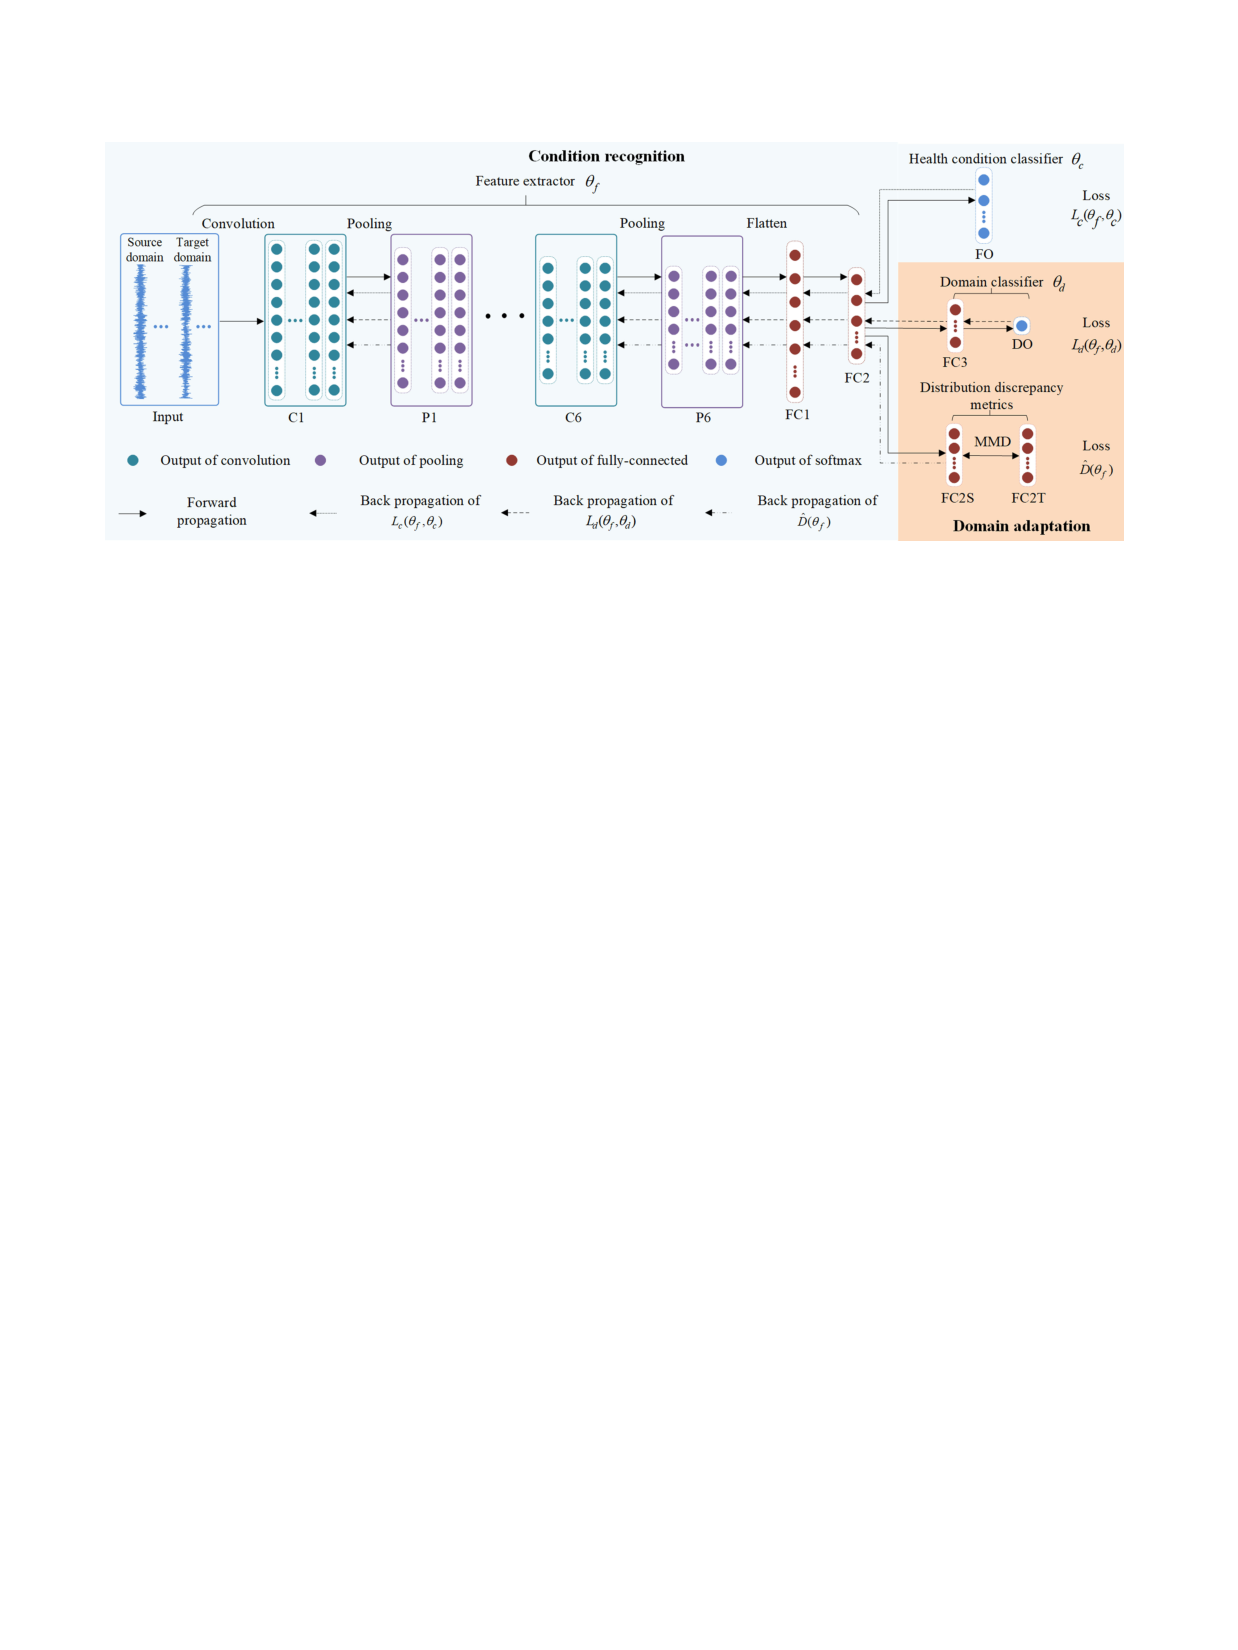
\includegraphics[width=1\textwidth]{models_state_of_the_art/DCTLN_model.pdf}
  \caption{DCTLN model \cite{Guo2019}}
  \label{fig:DCTLN_model}
\end{figure}

\subsection{Domain Conditioned Adaptation Network (DCAN)}
Most domain adaption approaches reduce the domain discrepancy in task-specific layers but use a shared feature extractor backbone across all domains. Li et al \cite{li2020} assume that these methods can only reduce the domain discrepancy, but not fundamentally eliminate it, if the domain discrepancy is tremendously large. Since the source and target domain are distributed differently and the models are just optimized for the supervised source domain, the CNN learns to extract features which are sensitive for the source domain but might not work as well with the target domain. Therefore, Li et al recommend to extract domain-specific and -independent features in the feature extractor backbone. 
Since the source and target domains are correlated in makes sense to use domain-indepent features to profit from the powerful feature extraction learned from the source even when processing target domain data. Additionally the model adapts the feature extractor to capture domain-specific features in the convolutional layers to improve the cross-domain feature alignment in the task-specific layers. Additionally, the extracted features are adjusted by the Domain Conditioned Feature Correction Module with the goal to reduce the domain discrepancy. The model is optimized with a regular source cross-entropy loss. Besides that a target entropy loss, which is formulated as following: 

\begin{equation}
    \min_{G} L_{s} = -\frac{1}{n_{t}} \sum_{j=1}^{n_{t}} \sum_{k=1}^{C_{t}} G^{(k)}(\pmb{x}_{tj})logG^{(k)}(\pmb{x}_{tj}),
\end{equation}
where $G(\dot)$ is the learned predictive model, $n_{t}$ is the number of source domain samples, $C_{n}$ are the classes present in source and target domain and $\pmb{x}_{t}$ are target samples.


The presented model is developed for computer vision applications and not predictive maintenance. Since predictive maintenance suffers from similar problems, this approach might be relevant for the community. The model is visualized in fig. \ref{fig:DCAN_model}. In the following the two domain adaption modules are described in more detail \cite{li2020}. 

\subsubsection{Domain Conditioned Channel Attention Mechanism}
Li et al \cite{li2020} use ResNet as backbone network which allows easy implementation of domain conditioned channel attention module in of it's residual block. In the latent layers of the DCAN model the processed images are represented in the form $\pmb{X}_{t} = [X^{1}_{t},...,X^{C}_{t}] \in \mathbb{R}^{HxWxC}$,where H and W are the spatial dimension and C the number of channels of the image. In the Domain Conditioned Channel Attention Module a channel-wise global average pooling layer is applied which reduces the images to  $\pmb{g}_{t} = [g^{1}_{t},...,g^{C}_{t}] \in \mathbb{R}^{1x1xC}$. Depending on the domain the data is passed through different fully connected layers. The upper flow is used for target and the lower flow for source samples. The two different source and target domain routes share parameters. For both domains the attention mechanism is learned jointly in order to learn to activate different channels for the domains, which allows extracting enriched domain specific features. In the fully connected layers the dimensionality is first reduced with a ratio ${1x1x\frac{C}{r}}$ and later reconstructed to its original size ${1x1xC$. Also in this context Relu and Sigmoid functions are applied. The domain-wise feature selection is achieved by weighting the channels of the original feature $\pmb{X}_{s}$ and $\pmb{X}_{t}$ with the resulting channel attention vectors $\pmb{v}_{s}$ and $\pmb{v}_{t}$ from the Domain Conditioned Channel Attention Module:

\begin{equation}
    \begin{aligned}
        &\pmb{\tilde{X}}_{s} = \pmb{v}_{s} \odot \pmb{X}_{s} = [v_{s}^{1} \cdot X_{s}^{1}, ..., v_{s}^{C} \cdot X_{s}^{C}]\\
        &\pmb{\tilde{X}}_{t} = \pmb{v}_{t} \odot \pmb{X}_{t} = = [v_{t}^{1} \cdot X_{t}^{1}, ..., v_{t}^{C} \cdot X_{t}^{C}].
    \end{aligned}
\end{equation}

The convolutional layers are activated by the channel attention vectors allowing the model to independently learn the importance of each channel for the source and target domain \cite{li2020}.

\subsubsection{Domain Conditioned Feature Correction}
A feature correction block is placed after each of the L task-specific layers. At the feature correction blocks the data simultaneously passes through the regular network but and the feature correction block, which consits of FC and Relu blocks. The feature correction block estimates the domain discrepancy in the feature representation of the corresponding task-specific layer:
\begin{equation}
    \Delta H_{l}(x_{t}) = H_{l}(x_{s}) - H_{l}(x_{t}),
\end{equation}
where $H_{l}(x_{s})$ and $H_{l}(x_{t})$ are the feature representations of the source and target domain samples in the task-specific layer L and $\pmb{x}_{s}$ $\pmb{x}_{t}$ are source and target domain samples. The feature representation of this layer is then modified as following:
\begin{equation}
    \hat{H}_{l}(x_{t}) = H_{l}(x_{t}) + \delta H_{l}(x_{t}).
\end{equation}
The MMD loss is applied using the feature representations $\hat{H}_{l}(x_{t})$ and $H_{l}(x_{s})$:

\begin{equation}
    L_{M}^{l} = |\frac{1}{n_s} \sum_{i=1}^{n_{s}} \phi(H_{l}(x_{si}) - \frac{1}{n_t} \sum_{i=1}^{n_{t}} \phi(\hat{H}_{l}(x_{ti}))|, 
\end{equation}
where Hκ is the reproducing kernel Hilbert space (RKHS) using the characteristic kernel κ, a corresponding feature map φ and $n_{t}$ are the number of target samples. Reducing the domain discrepancy improves the feature transferrability but also transfers  noise and unimportant information between the domains, which destroys the structure of the source and target domain data, making the classification task more difficult. To avoid this over-transfer between source and target, the model should be enforced to keep the source data constant when passing through the feature correction blocks. Since $\Delta H_{l}(x_{s}) \approx 0$ would prevent the cross-domain feature correction. To tackle that problem a regularization attempts to minimizes the MMD loss between samples of a random subset of source samples corresponding to each class:
\begin{equation}
    L_{reg}^{l} = \sum_{k=1}^{C_{n}}|\frac{1}{n_{s}^{k}} \sum_{x_{si} \in S^{k}} \phi(H_{l}(x_{si})) - \frac{1}{|R|} \sum_{x_{sj} \in R} \phi(\hat{H}_{l}(x_{sj}))|_{Hk}^{2}, 
\end{equation}
where $R$ is a random subset in the source domain samples and $S^{k}$ is the set of source domain samples belonging to class k \cite{li2020}.

\begin{figure}[p]
  \centering
  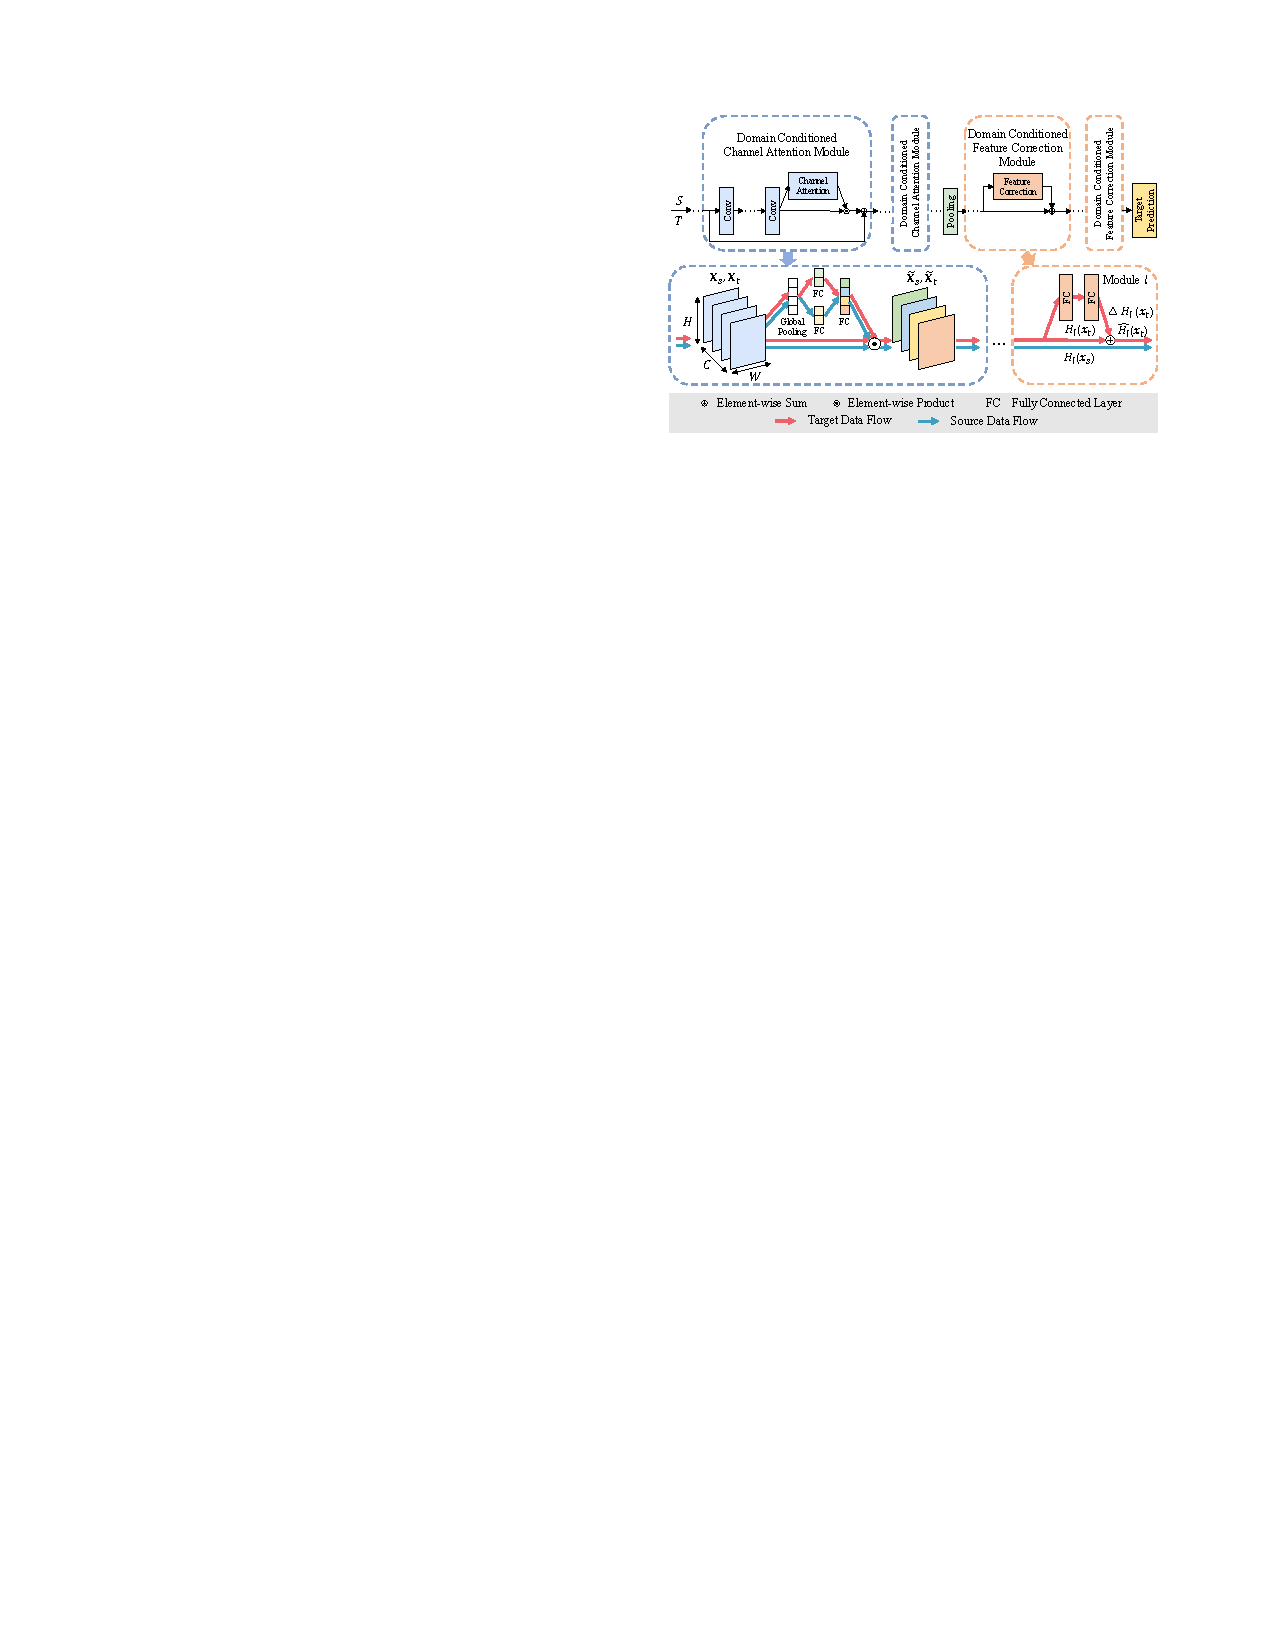
\includegraphics[width=1\textwidth]{models_state_of_the_art/DCAN_model.pdf}
  \caption{DCAN model \cite{li2020}}
  \label{fig:DCAN_model}
\end{figure}

\subsection{Deep belief networks}
A domain adaption algorithm based on DBNs which uses wavelet transforms as a preprocessing step was proposed by Zang et al \cite{Zhang2017}. Degradation of ball screws lead to decreased stiffness in the system which increases vibrations. Using vibration signals are promising to evaluate the degradation state of the ball screw. The packet energy of the wavelet transform shows an exponential increase trend with increasing degradation and is therefore a good indicator for the degradation level. Multi-sensor data fusion is a method to synthesize data from different sources in order to generate a better basis for decisions. The proposed method presented by Zang et al is visualized in fig. \ref{fig:Deep_belief_networks_model} and described the following step by step:

\begin{itemize}
    \item [1.] N signals are collected with sensors mounted at different positions of the machine.
    \item [2.] The frequency spectrum $\{f_{(1)}^{i}, ..., f_{(N)}^{i}\}_{i=1}^{M}$ is calculated for each of the N extracted time-domain signals using wavelet transform, where M is the number of degradation samples.
    \item [3.] Fuse the frequency spectrum of the N signals $\{F^{i}\}_{i=1}^{M}$, where $F^{i}=f_{(1)}^{i} \cap ... \cap f_{(N)}^{i}$. In the end the fused frequency spectrum is normalized by its dimension, which can be expressed as $dim(F^{i})=\sum_{j=1,...,N} dim(f_{(j)}^{i})$.
    \item [4.] Pre-train the DBN by applying the regular RBM training (iteratively apply positive and negative phase) to each layer. The fused frequency spectrums are used for the unsupervised training. 
    \item [5.] Separate the level of degradation in classes and obtain the output dimension of the model.
    \item [6.]  Fine-tune the deep belief network with the supervised back-propagation training algorithm. The error between the true and predicted degradation class is minimized.
    \item [7.] Apply the model as intelligent degradation monitoring system in order to estimate the degradation level of unseen data samples \cite{Zhang2017}.
\end{itemize}

\begin{figure}[p]
  \centering
  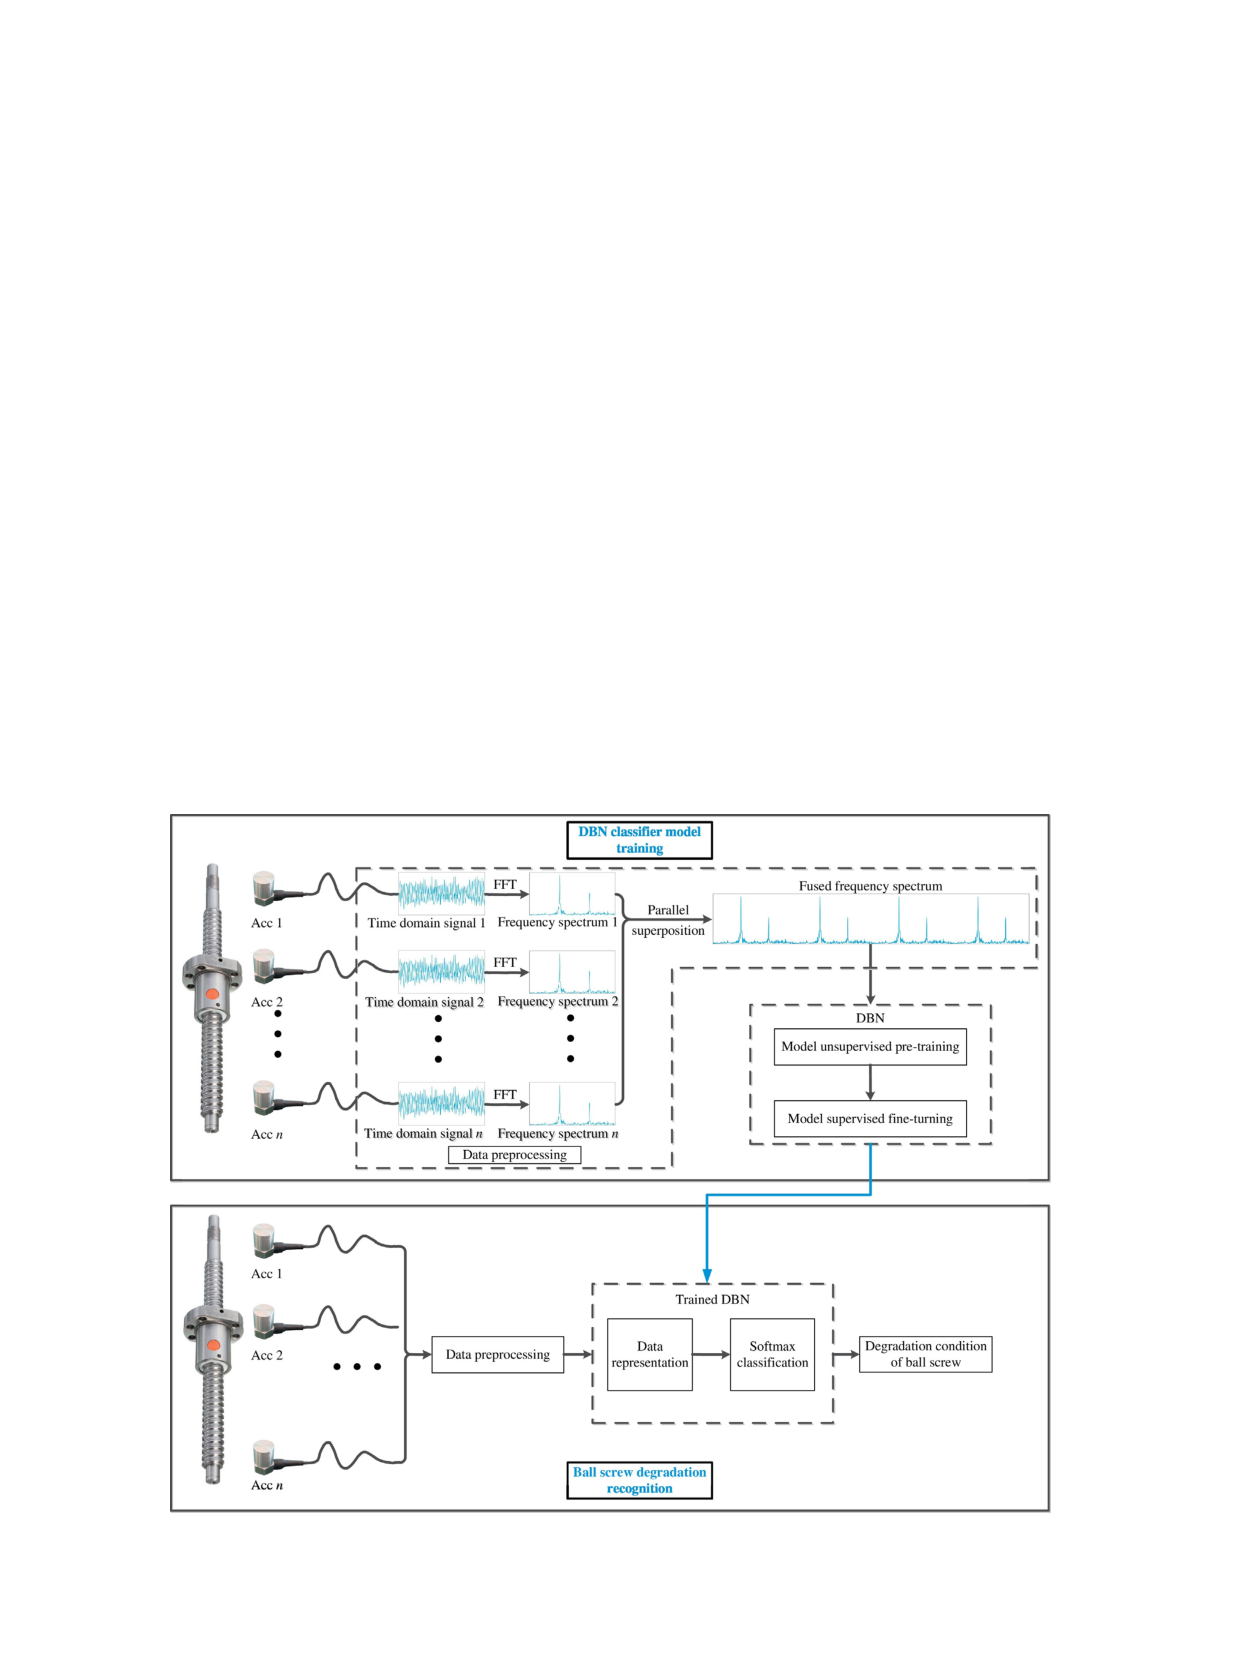
\includegraphics[width=1\textwidth]{models_state_of_the_art/Deep_belief_networks_model.pdf}
  \caption{Deep belief networks model \cite{Zhang2017}}
  \label{fig:Deep_belief_networks_model}
\end{figure}



\subsection{Wasserstein distance guided multi-adversarial networks (WDMAN)}
\cite{Zhang2019}


\chapter{Research Approach}\label{chapter:research_approach}
\chapter{Experiments and Methods}\label{chapter:experiments}

\section{Experimental Setup: Ball Screw Drive}
Data from a DMG DMC 55H duoblock milling machine of the manufacturer DMG Mori were collected to evaluate different PHM approaches. The machine tool’s spindle and housing, as well as the machine tool table, rotatory axes, peripherals, the cladding and the machine tool's housing were removed. The TNC control iTNC530 HSCI from Heidenhain GmbH was used. The focus of the experiments is to investigate how different levels of abrasion of the linear guiding shoes (LGSs) affect the prediction of the health condition states of the ball screw drives (BSDs) in the machine. Besides the regular preload loss due to abrasion, the BSDs also show pitting damages. For this reason, the health condition classes of BSDs are separated in pitting damage (D) and no pitting damage (C). For the LGSs just no pitting damages (C) were observed. The health condition state of BSDs and LGSs is specified by one letter and two digits. The letter indicates the damage type (C or P), the first digit specifies the preload class and the second digit the number of the observation. In the experiments, three classes were differed, indicating the preload force within the component and therefore its level of abrasion. Low preload forces indicate stronger abrasion, leading to lower machine precision and higher risk for failure. Preload class C3 were labelled as “healthy”, C2 as "slightly degraded" and C1 as "strongly degraded". The experiments, which combine different LGS and BSD states, were repeated. The observation digit specifies different experiments with equal LGS and BSD setups. An overview over the tracked health condition states of the BSDs and LGSs is visualized in table \ref {tab:BSDs_states} and table \ref {tab:LGSs_states}. The ID specifies the health condition state of the BSD or LGS with one digit and two numbers as described before. The component name identifies the exact machine part evaluated in that experiment. Since one experiment contains two LGSs, consisting of two parts each, and one BSD threaded shaft, each BSD ID maps to one and each LGS ID to four components. The preload for the BSD and LGS is measured as force (N).


\begin{center}
\begin{longtable}{c c c} 
\toprule
 ID & Component & Preload in N \\ [0.5ex] 
\midrule
 P1 & 721-14448-6-G6 & 2 070 \\ 
 P2 & 721-14448-4-G4 & 2 160 \\ 
 C11 & 721-14448-3-G3 & 2 950 \\ 
 C12 & 721-95859-4 & 845 \\ 
 C21  & 721-14448-1-G1 & 1 450 \\ [1ex] 
 C22  & 721-95859-2 & 1 293 \\ [1ex] 
 C31  & 721-14448-2-G2 & 2 390 \\ [1ex] 
 C32  & 721-95859-3 & 2 328 \\ [1ex] 
 C33 & 721-95859-1 & 2 031 \\ [1ex]
\bottomrule
\caption {BSDs States}
\label {tab:BSDs_states}
\end{longtable}
\end{center}


\begin{center}
\begin{longtable}{c c c} 
\toprule
 ID & Component & Preload in N \\ [0.5ex] 
\midrule
 C1 & C1 & 4 060 \\ 
    & C2 & 4 430 \\ 
    & C3 & 4 430 \\
    & F1 & 3 880 \\ 
\midrule
 C2 & B1 & 8 860 \\ 
    & B2 & 9 700 \\ [1ex] 
    & B3 & 9 070 \\ [1ex]
    & E1 & 8 230 \\ [1ex]
\midrule
 C3 & A9 & 13 470 \\ 
    & A10 & 14 530 \\ [1ex] 
    & A11 & 12 840 \\ [1ex]
    & D3 & 12 840 \\ [1ex]
\bottomrule
\caption {LGSs States}
\label {tab:LGSs_states}
\end{longtable}
\end{center}

Fig. \ref{fig:experimental_setup} shows the experimental setup. The investigation focuses on the moving hanger assembly of the machine tool. The machine tool can be moved in the three spatial directions. The experiments are restricted to the movement of the machine tool along the x-axis. For this reason, just the single threaded shaft of the BSD and the two counterparts each belonging to one of the two LGSs are supervised.

\begin{figure}[H]
  \centering
  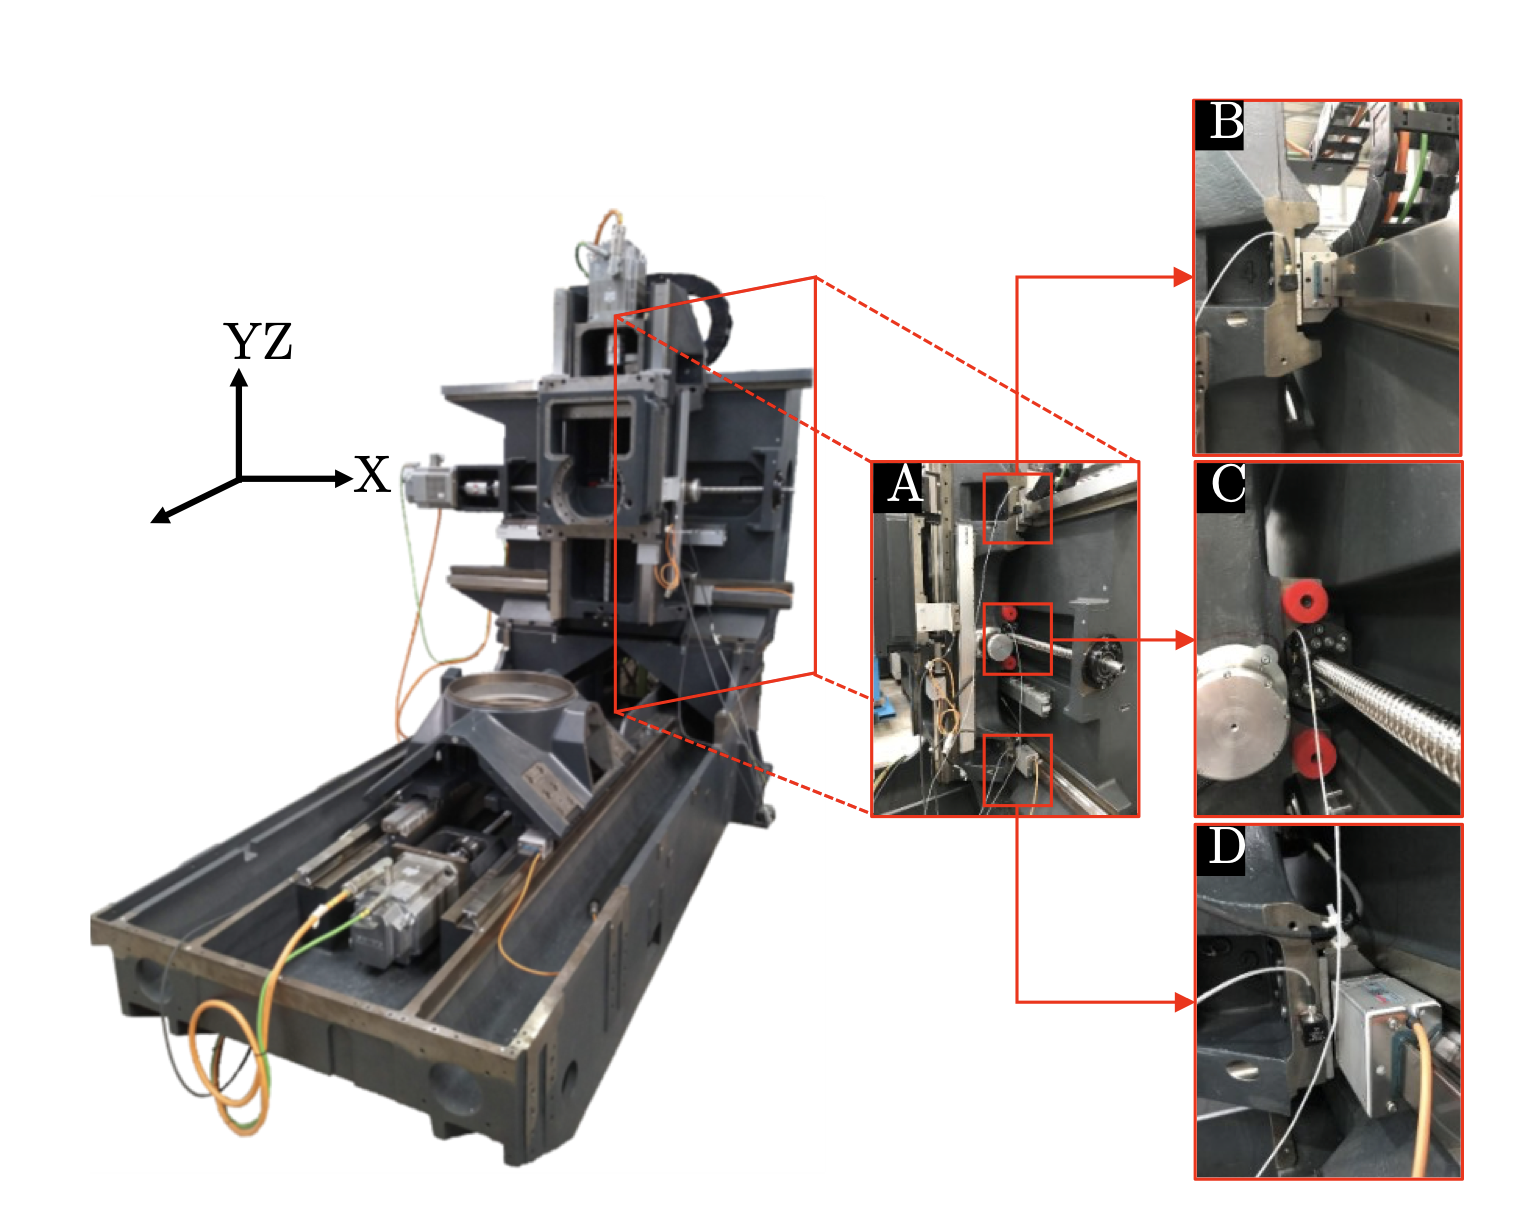
\includegraphics[width=0.9\textwidth]{experimental_setup}
  \caption {Experimental Setup: A: side-view of the machine, B: Upper LGS, C: Threaded Shaft of BSD, C: Lower LGS}
  \label{fig:experimental_setup}
\end{figure}

The software tool TNC Scope uses an oscilloscope to provide internal control data. Three triaxial Kistler 8762A10 piezo-eletric accelerometers are mounted at different positions (bottom, nut, top) and track the accelerations in all spatial directions when moving the machine tool along the x-axis.

\section{Dataset: Ball Screw Drive}
For the sake of reproducibility, the experiments are executed with a defined test cycle, which is defined in fig. \ref{fig:test_cycle}. Machine data is collected during constant speed, direction change and sweep excitement along the machine tools X-axis. During the constant speed excitement, the machine tools are moved back and forth along the whole axis ($\Delta x$ = 600mm). During the direction change excitation, the movement of the machine tools is restricted to a small part of the axis ($\Delta x$ = 1mm) and the directions are changed with a high frequency. In the sweep excitement, the motor, moving the machine tools along the different axis, receives a target speed in the form of a sine sweep. Before recording data, the machine is warmed up to create equivalent circumstances for each run. A constant speed excitement is applied for 60 min. 

\begin{figure}[H]
  \centering
  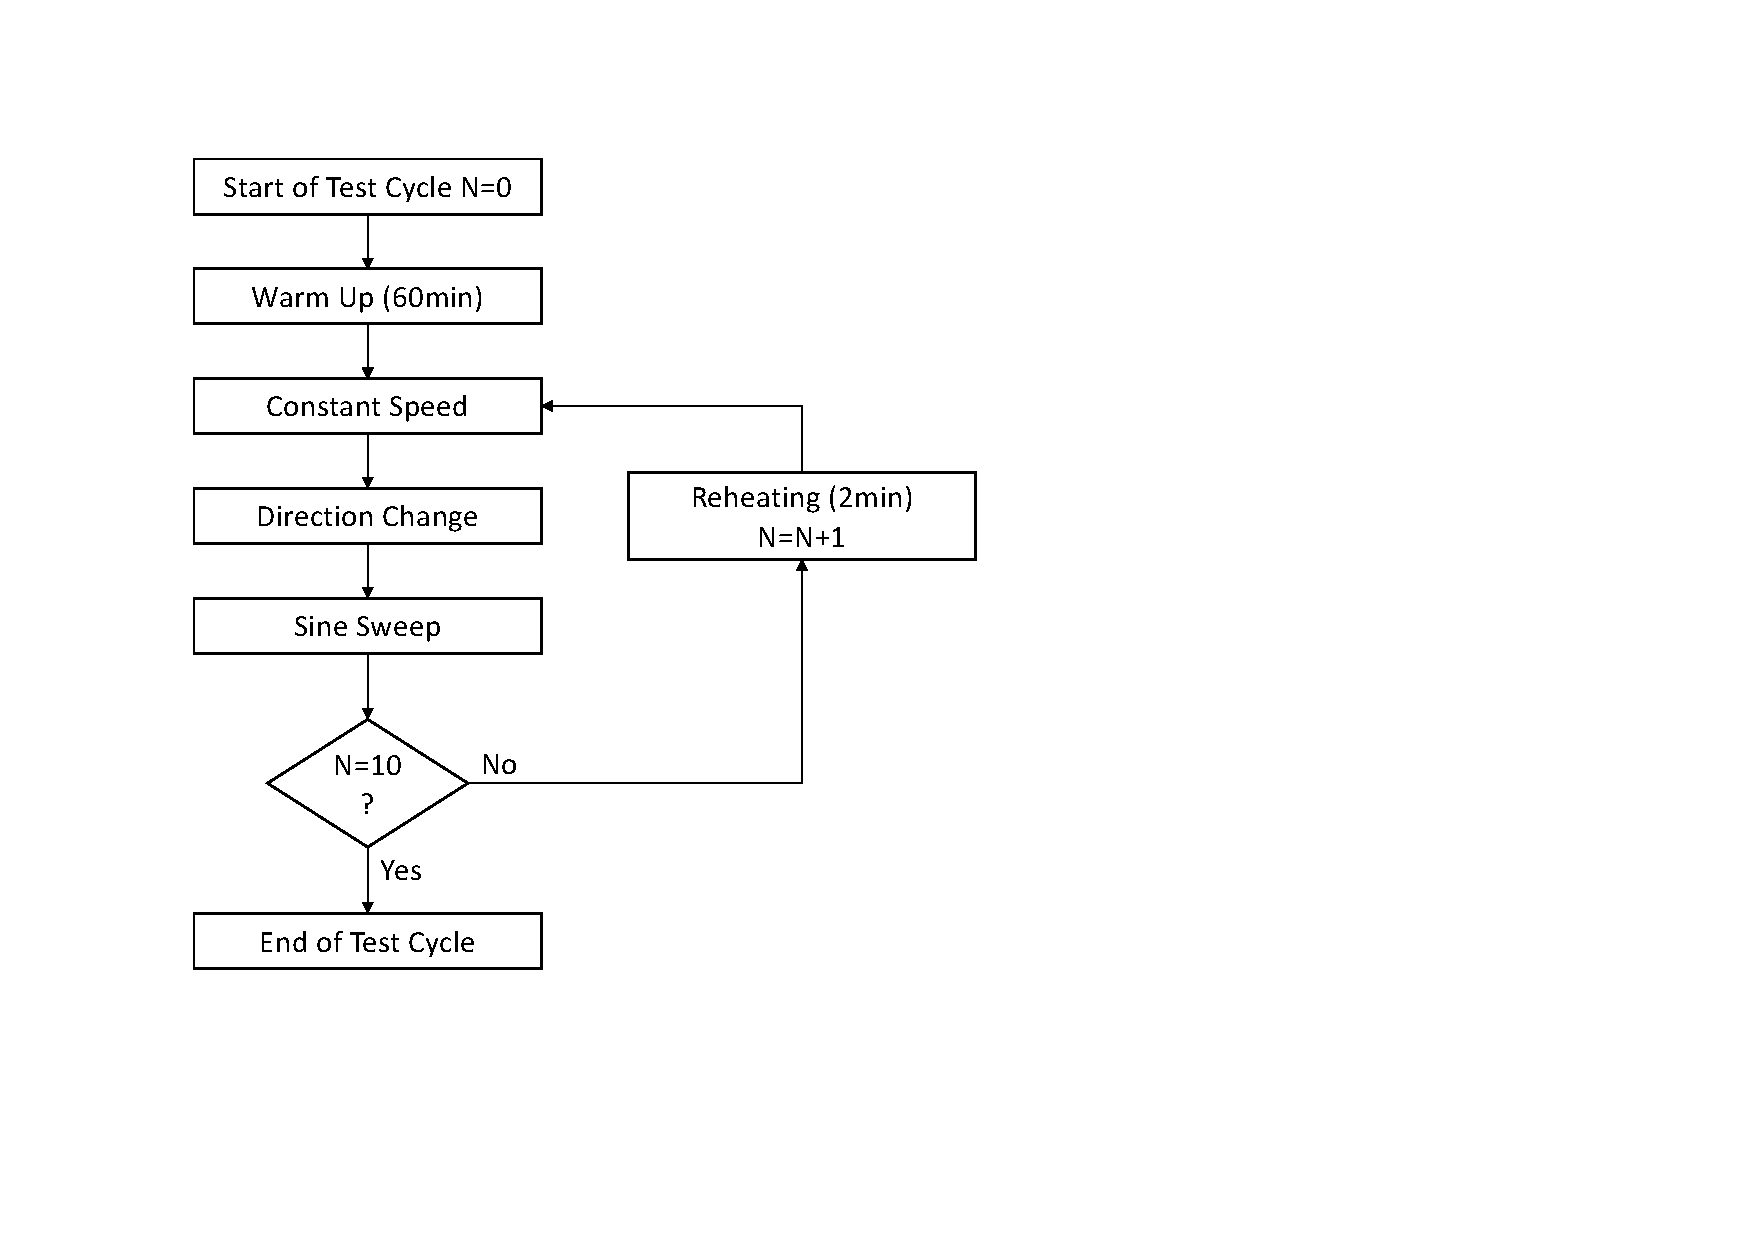
\includegraphics[width=0.7\textwidth]{test_cycle.pdf}
  \caption {Test Cycle for Recording the Dataset}
  \label{fig:test_cycle}
\end{figure}

In total 49 different signals are recorded during one sub cycle. The signals are specified in more detail in table. \ref{tab:description_of_the_49_recorded_features}. All feature names starting with "C" correspond to the constant speed , "D" to the direction change and "S" to the sweep excitement.

\begin{center}
\begin{longtable}{c c c c} 
 \toprule
 Signal & Sensor & Frequency & Samples \\ [0.5ex] 
 \midrule
 C:s ist/X & TNC Scope & 10 kHz & 75000 \\ 

 C:s soll/X & TNC Scope & 10 kHz & 75000 \\ 

 C:s diff/X & TNC Scope & 10 kHz & 75000 \\ 

 C:v (n ist)/X & TNC Scope & 10 kHz & 75000 \\ 

 C:v (n soll)/X& TNC Scope & 10 kHz & 75000 \\ 

 C:P mech./X & TNC Scope & 10 kHz & 75000 \\ 

 C:Pos. Diff./X & TNC Scope & 10 kHz & 75000 \\ 

 C:I ist/X & TNC Scope & 10 kHz & 75000 \\ 

 C:I soll/X & TNC Scope & 10 kHz & 75000 \\ 

 C:x bottom & Acc & 10 kHz & 75000 \\ 

 C:y bottom & Acc & 10 kHz & 75000 \\ 

 C:z bottom & Acc & 10 kHz & 75000 \\ 

 C:x nut & Acc & 10 kHz & 75000 \\ 

 C:y nut & Acc & 10 kHz & 75000 \\ 

 C:z nut & Acc & 10 kHz & 75000 \\ 

 C:x top & Acc & 10 kHz & 75000 \\ 

 C:y top & Acc & 10 kHz & 75000 \\ 

 C:z top & Acc & 10 kHz & 75000 \\ 

 D:s ist/X & TNC Scope & 10 kHz & 75000 \\

 D:s soll/X & TNC Scope & 10 kHz & 75000 \\ 

 D:s diff/X & TNC Scope & 10 kHz & 75000 \\ 

 D:v (n ist)/X & TNC Scope & 10 kHz & 75000 \\ 

 D:v (n soll)/X & TNC Scope & 10 kHz & 75000 \\ 

 D:P mech./X & TNC Scope & 10 kHz & 75000 \\ 
 
 D:Pos. Diff./X & TNC Scope & 10 kHz & 75000 \\ 

 D:I ist/X & TNC Scope & 10 kHz & 75000 \\ 

 D:I soll/X & TNC Scope & 10 kHz & 75000 \\ 

 D:x bottom & Acc & 10 kHz & 75000 \\ 

 D:y bottom & Acc & 10 kHz & 75000 \\ 

 D:z bottom & Acc & 10 kHz & 75000 \\ 

 D:x nut & Acc & 10 kHz & 75000 \\ 

 D:y nut & Acc & 10 kHz & 75000 \\ 

 D:z nut & Acc & 10 kHz & 75000 \\ 

 D:x top & Acc & 10 kHz & 75000 \\

 D:y top & Acc & 10 kHz & 75000 \\ 

 D:z top & Acc & 10 kHz & 75000 \\ 

 S:x bottom & Acc & 10 kHz & 153601 \\ 

 S:y bottom & Acc & 10 kHz & 153601 \\ 

 S:z bottom & Acc & 10 kHz & 153601 \\ 

 S:x nut & Acc & 10 kHz & 153601 \\ 

 S:y nut & Acc & 10 kHz & 153601 \\ 

 S:z nut & Acc & 10 kHz & 153601 \\ 

 S:x top & Acc & 10 kHz & 153601 \\ 

 S:y top & Acc & 10 kHz & 153601 \\ 
 
 S:z top & Acc & 10 kHz & 153601 \\ 
 
 S:Nominal rotational speed & TNC opt & 1 kHz & 16384 \\
 
 S:Actual rotational speed & TNC opt & 1 kHz & 16384 \\ 
 
 S:Actual position of the position encoder(dy/dt) & TNC opt & 1 kHz & 16384 \\ 
 S:Actual position of the motor encoder(dy/dt)  & TNC opt & 1 kHz & 16384  \\ [1ex] 
 \bottomrule
\caption {Signal Description}
\label {tab:description_of_the_49_recorded_features}
\end{longtable}
\end{center}

Due to abrasion, the different machine components wear down. LGSs are separated in three and the BSDs in four different health condition classes. Usually, the lifetime of BSDs is shorter than that of the LGSs. This means that ball screws need to be replaced in shorter internals. Different combinations of LGSs and BSDs health condition classes were recorded, which are shown in the following table. \ref{tab:recorded_combinations_of_LGS_and_BSD_health_conditions}

\begin{table}[ht]
  \large
  \centering
  \begin{tabular}{c|c||*{9}{c|}}
    \multicolumn{2}{c}{} & \multicolumn{9}{c}{BSD} \tabularnewline
    \cline{2-11}
    \multirow{5}*{\rotatebox{90}{LGS}} &
&    \bfseries C31 & \bfseries C21 & \bfseries C11 & \bfseries P1 & \bfseries C22 &\bfseries C12 & \bfseries C32 &\bfseries C33 &\bfseries P2  \tabularnewline[1 ex] 
\cline{2-11}
&    \bfseries C3 & 1 &  2 &  3 & 4 & 5 & 6 & 7 & 8 & 9 \tabularnewline [1ex] 
    \cline{2-11}
&    \bfseries C2 & 10 &  11 &  12 &  13 & 14 & 15 & 16 & 17 & 18\tabularnewline [1ex] 
    \cline{2-11}
&    \bfseries C1 & 18 & 19 & 20 & 21 & 23 & 24 & 25 & 26 & 27 \tabularnewline [1ex] 
    \cline{2-11}
  \end{tabular}
\caption {Combinations of LGS and BSD Health Conditions}
\label {tab:recorded_combinations_of_LGS_and_BSD_health_conditions}
\end{table} 

For the experiments, two domains were defined. The source domain consists of the health condition states 2, 3, 11, 12, 20, 21 and the target domain of 5, 6, 14, 15, 23, 24. The model is trained to predict the health condition class of the BSD. Both the source and target domain includes the four BSD health condition classes C1, C2, C3 and P1 combined with all three LGS preload classes C1, C2, C3. In order to generate a binary classification problem, the BSD states C1 and P1 were combined as "healthy" and C2 and C3 as "degraded" class. The source and target domain includes the same combination of BSD and LGS health condition classes, just from two different observations (source: observation 1, target:observation 2). In both observations, the used LGSs are the exact same components, but Contrariwise, different BSD components with similar degradation levels were used. The defined health condition classes of the BSDs are defined differently for the two observations. Table \ref {tab:BSDs_states} shows that the defined preload for C11 and C12, C21 and C22, C31 and C32 as well as P1 and P2 differ with up to 147 N. This inhomogeneous definition of the BSD health condition classes as well as marginal differences in the production and installation of the BSDs leads to a significant domain shift problem, which affects the performance of the model during the testing enormously. 


\section{Dummy Dataset}
The applicability of different domain-adaption approaches in the context of PHM was evaluated on a synthetic dummy dataset, which is structured equally and shows similar patterns as the corresponding real-world dataset. The complexity of the data and therefore the task can be tuned arbitrarily. A dataset like that can help to understand underlying mechanisms of new and unknown approaches. Besides that, it serves as a prior evaluation for the approach's applicability for a given real-world task. In this work, a simple dummy dataset was established to evaluate the MMD loss to learn a more domain-invariant feature extraction. Since one has to deal with irregularities, outliers and noise in real-world data, it is helpful to evaluate the MMD loss on a dataset which is not disturbed by these effects. Similarly to PHM applications, the model in the dummy dataset processes time sequences. In the dummy example, the time sequences consist of 1000 data points which are sampled from a cosine  curve. The synthetic dataset which simulates the classification problem with two classes and two domains is sampled from four cosine  curves, each with characteristic amplitudes and frequencies. By adjusting the amplitude and frequency, the domain adaption problem can be configured more or less difficult. The sampling process must include a certain randomness to allow differing sequences for the same class and domain. For every sampling step, the domain- and class-specific amplitude and frequency of the cosine  curve is perturbed. This changes the underlying characteristic of each sequence. Besides that, noise is added to each of the 1000 data points within that sequence. This is necessary to generate a periodic signal which is close to a noisy real-world vibration signal. For the sake of simplicity, the dataset contains just 1-D sequences. This simulates a health monitoring task on just one single signal. In Fig. \ref{fig:samples_domain_class_dummy} four data sequences are shown representing one example sequence for each class and domain. 

\begin{figure}[H]
  \centering
  \includegraphics[width=.45\textwidth]{samples_domain_class_dummy/Source_Domain_Class_0_obs_0.pdf}
  \hspace{.3cm}
  \includegraphics[width=.45\textwidth]{samples_domain_class_dummy/Source_Domain_Class_1_obs_0.pdf}

  \vspace{.3cm}

  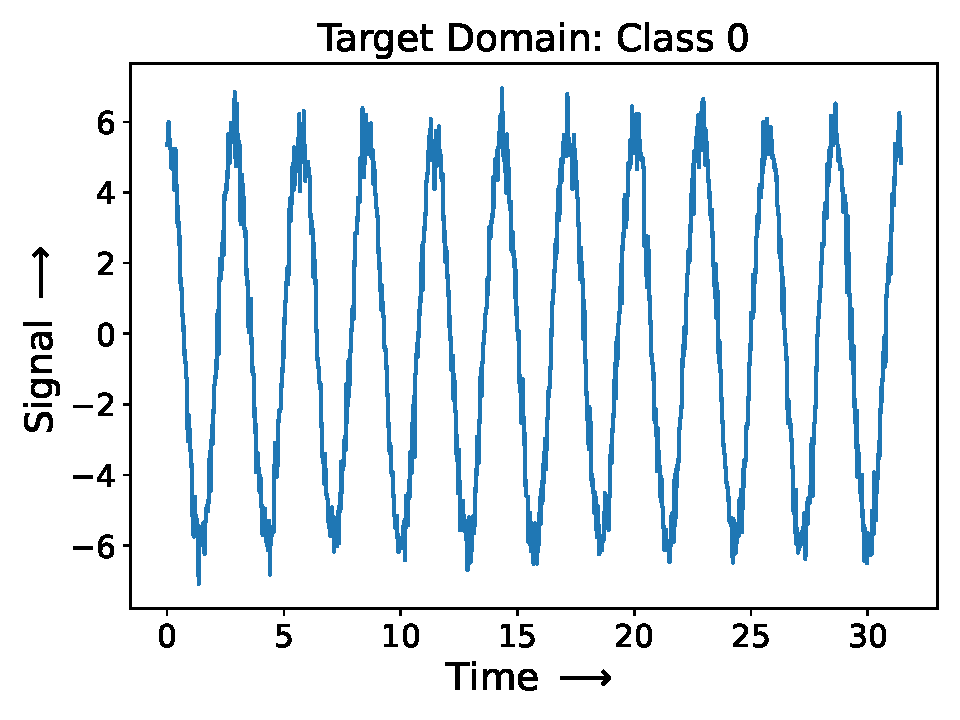
\includegraphics[width=.45\textwidth]{samples_domain_class_dummy/Target_Domain_Class_0_obs_0.pdf}
  \hspace{.3cm}
  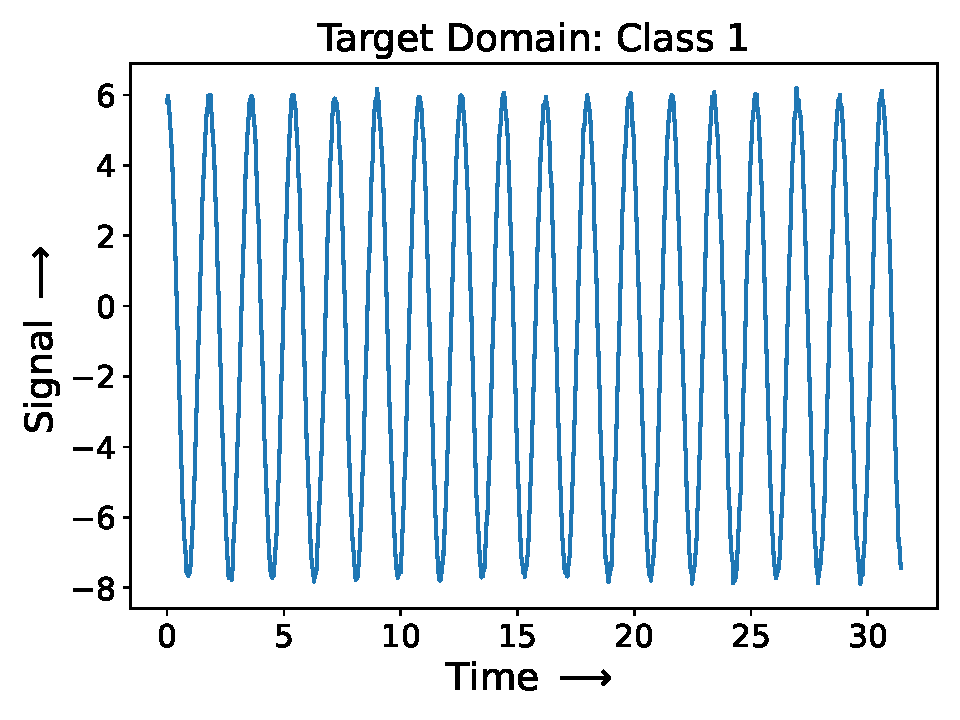
\includegraphics[width=.45\textwidth]{samples_domain_class_dummy/Target_Domain_Class_1_obs_0.pdf}

  \caption{Data Window Samples for each Domain and Class}
  \label{fig:samples_domain_class_dummy}
\end{figure}


In fig. \ref{fig:samples_domain_class_dummy_influence_noise} one can see how the applied perturbation and noise during the sampling process changes the data sequences belonging to the same class and domain. 


\begin{figure}[H]
  \centering
  \includegraphics[width=.45\textwidth]{samples_domain_class_dummy_influence_noise/Source_Domain_Class_0_obs_0.pdf}
  \hspace{.3cm}
  \includegraphics[width=.45\textwidth]{samples_domain_class_dummy_influence_noise/Source_Domain_Class_1_obs_0.pdf}

  \vspace{.3cm}

  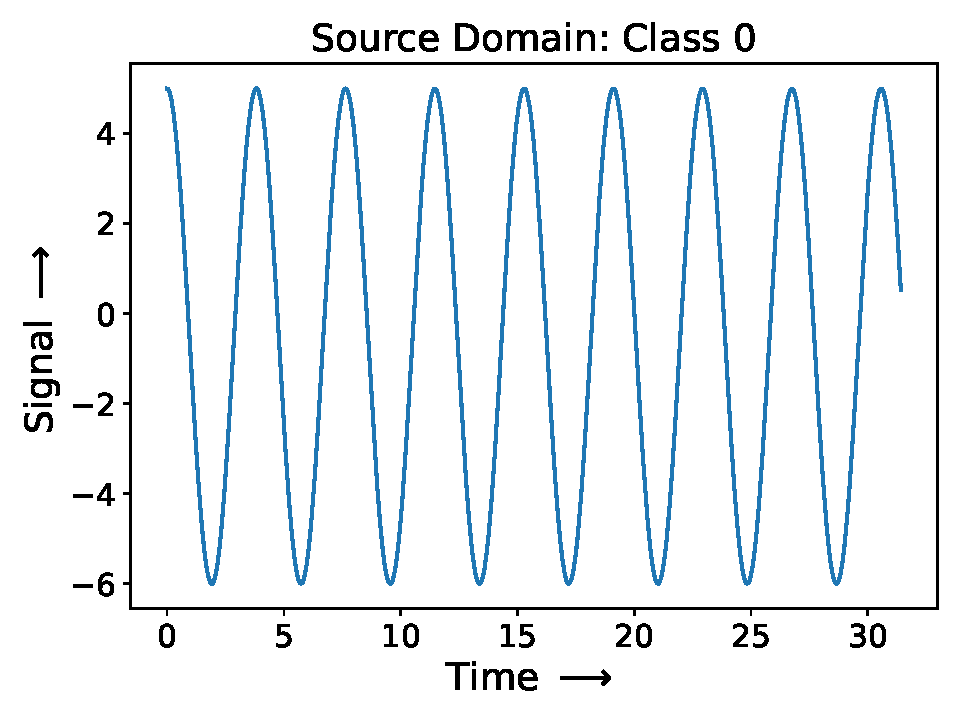
\includegraphics[width=.45\textwidth]{samples_domain_class_dummy_influence_noise/Source_Domain_Class_0_obs_1.pdf}
  \hspace{.3cm}
  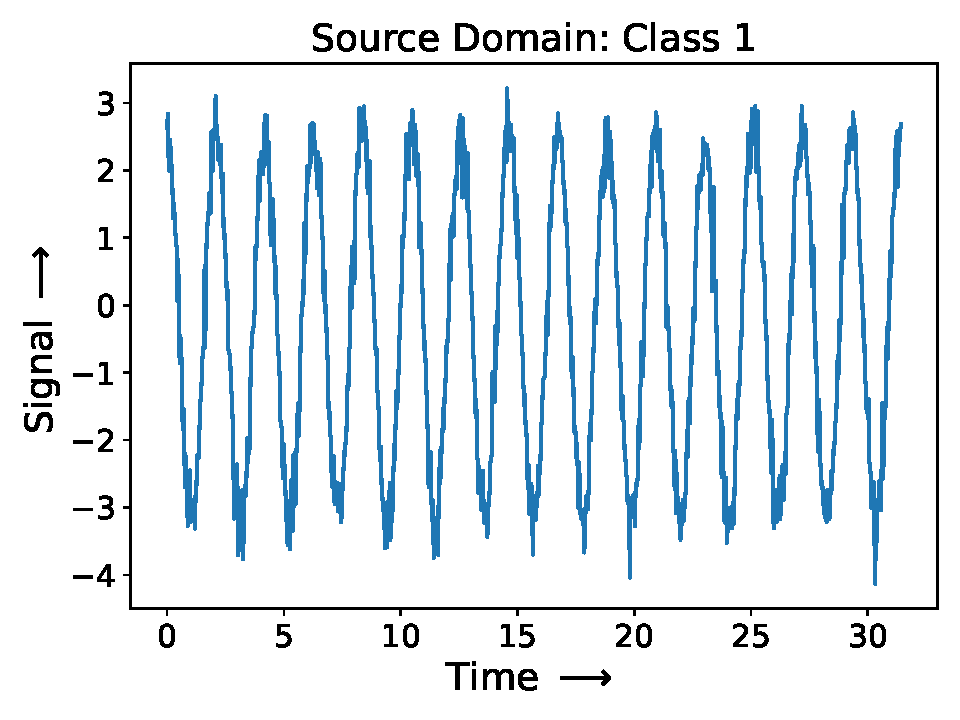
\includegraphics[width=.45\textwidth]{samples_domain_class_dummy_influence_noise/Source_Domain_Class_1_obs_1.pdf}

  \caption{Perturbation and Noise during Sampling Process}
  \label{fig:samples_domain_class_dummy_influence_noise}
\end{figure}



\section{Methods}\label{chapter:introduction}
In the following the model used in this thesis as well as the applied training concepts are presented

\subsection{Model}
\label{sec:model}
The model used during the experiments consists of a 1D CNN which is responsible to extract expressive features and a subsequent classifier predicting the health condition classes of the BSDs. A more detailed. visualization of the architecture is shown in fig.\ref{fig:proposed_model}. The CNN consists of 3 convolutional layers. With increasing network depth the spatial dimension of the feature map is decreased and its channel size increased. This helps to extract more global features in shallow and more specific and local features in deeper layers. The exact parameters of the convolutional layers are described in table \ref{tab:parameter_conv} 

\begin{longtable}{c c c c} 
\toprule
Parameter & Conv 1 & Conv 2 & Conv 3 \\
\midrule
kernel size & 100 & 10 & 5 \\

padding size & 0 & 1 & 1 \\

stride & 1 & 1 & 1 \\
\bottomrule
\caption {Parameter in Convolutional Layer}
\label {tab:parameter_conv}
\end{longtable}

Several pooling layers are included after the convolutional layers to reduce the spatial dimension of the feature maps. Reducing the model complexity prevents problems like overfitting and exploding gradients. Applying batch normalization after convolutional layers fixes the means and variances of the layers inputs for each batch, which helps to make the training faster and more stable. After iteratively applying these three types of layers the output of the CNN is flattened and normalized to a 1D vector. This vector is used as an input for the subsequent classifier. The latent feature space dimension of the classifier is reduced constantly. The two neurons in the output layer of the neural network represents the prediction probability for the two defined BSD health condition classes.


\begin{figure}[H]
  \centering
  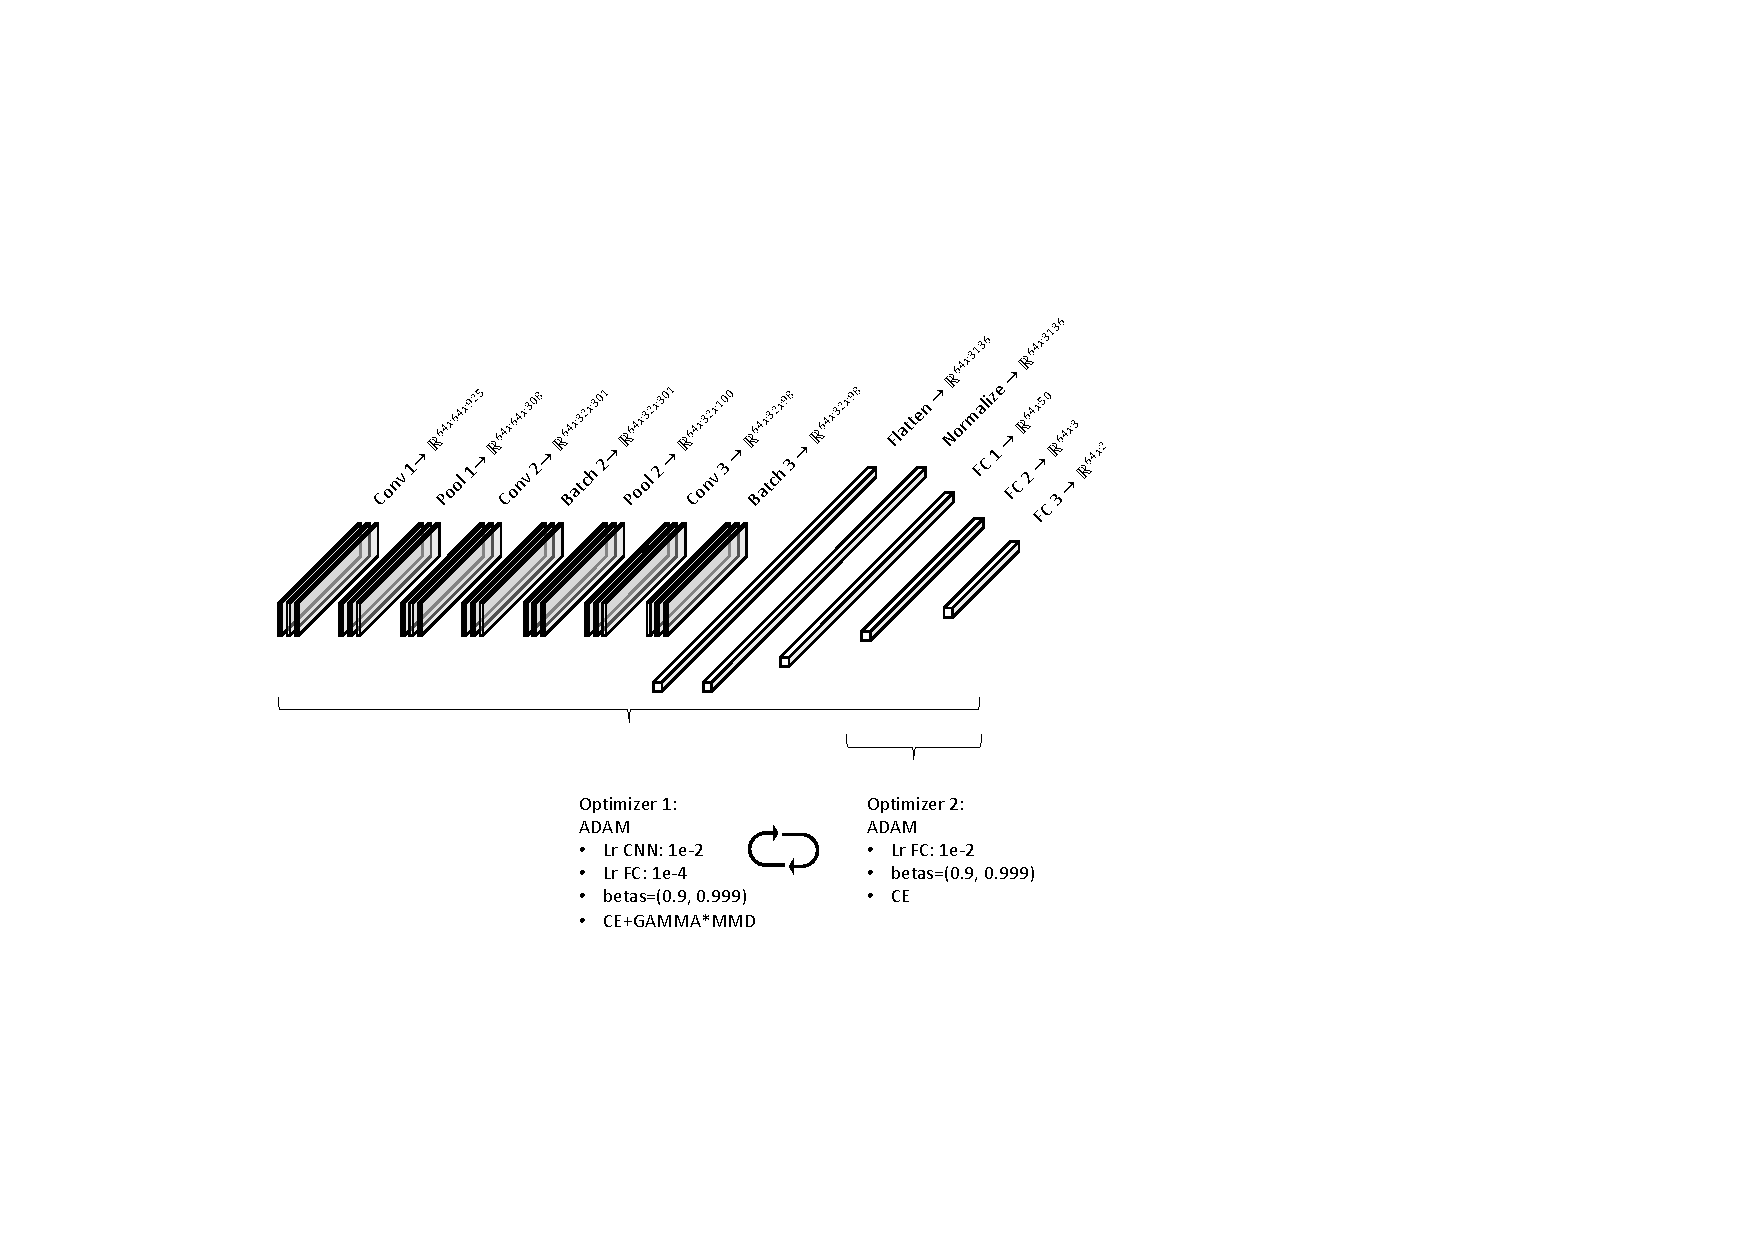
\includegraphics[width=1\textwidth]{proposed_model.pdf}
  \caption {Proposed Model} \label{fig:proposed_model}
\end{figure}


\subsection{Proposed Training with MMD and Cross Entropy Loss} \label{sec:Proposed_training}

Firstly, the data used for the training is pre-processed. A dataloader is used to prepare the dataset. In a first step, the data is separated in shorter sequences of length 1024. These windows, which can include several of the recorded 49 signals, are fed as samples to the model. The sequences are cleaned from Nan values and synchronized afterwards. The dataset is randomly separated in a train, validation and test set with a split of 60\%/20\%/20\%. Also, the application of wavelet transforms, which can generate more informative data for the model, was partially investigated in this step. The repetitive training of the model is visualized in fig. \ref{fig:Training_Process_MMD}. A combination of a source cross-entropy and a MMD loss is applied to optimize the proposed deep-learning based domain adaption model. The MMD loss estimates the domain discrepancy in several latent feature maps. The MMD loss facilitates the extraction of more domain independent features within the model's layers. The cross entropy loss trains the model to increase the classification accuracy on the source domain. The domain discrepancy is measured as squared distance between distribution kernel embeddings in the reproducing kernel Hilbert space (RKHS). For the performance of the MMD loss, the kernel choice is of great importance. For this reason, several RBF kernels with bandwidth parameters 1, 2, 4, 8, 16 were combined in order to profit from their individual strength. For applying the MMD loss, two samples from each, source and target domain, are sampled randomly. For each such generated pair of samples, the MMD loss is calculated. The class of each sample is not considered in the MMD loss. Therefore, the MMD loss minimizes the domain discrepancy based on the observed source and target sample pairs, which partially belong to different but also to the same classes. The MMD is applied in several layers of the CNN and classifier. The source cross entropy loss is applied in the final layer. Fig. \ref{fig:MMD_Loss_and_CE_loss} symbolically shows how the MMD and the source cross-entropy loss is extracted from the different layers of the model.

\begin{figure}[H]
  \centering
  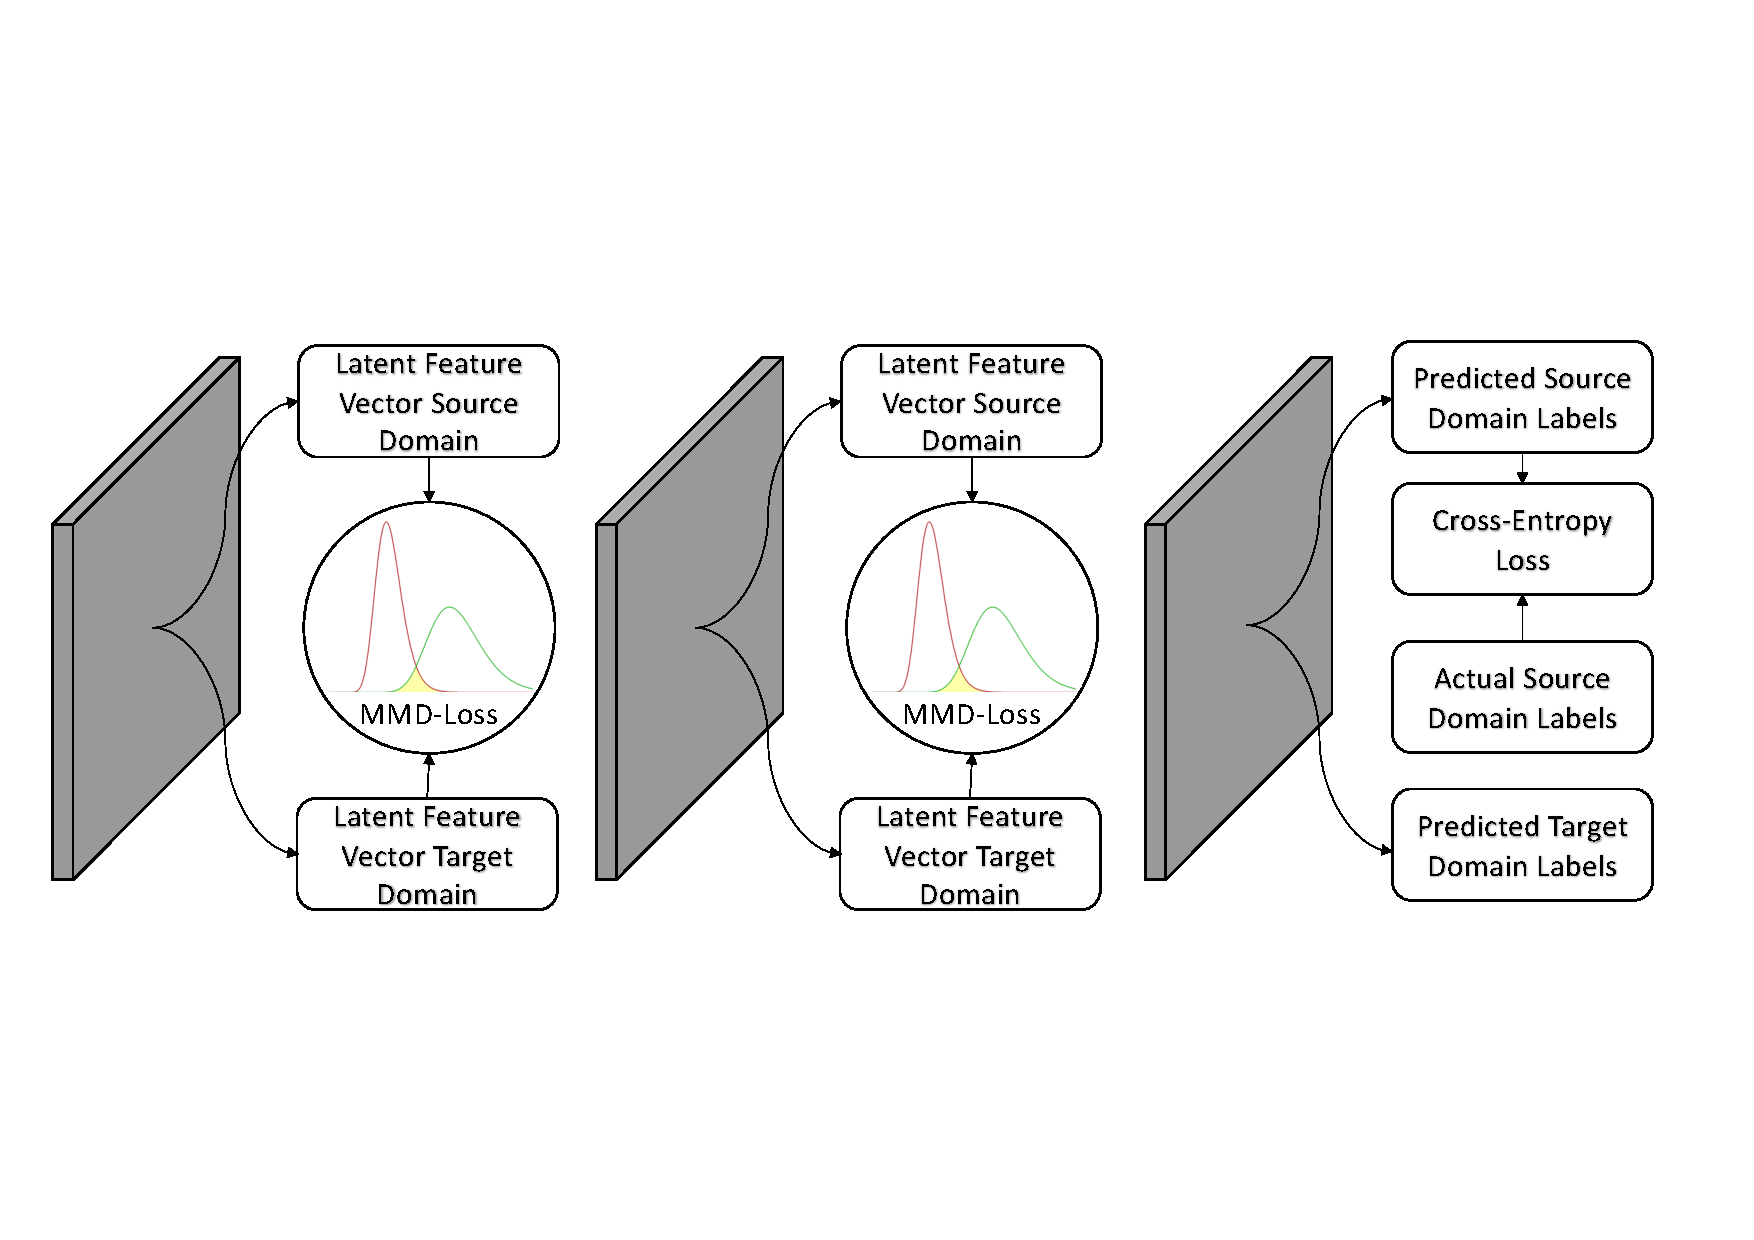
\includegraphics[width=1\textwidth]{MMD_loss_visualization.pdf}
  \caption {Cross Entropy Loss and MMD Loss in Neural Networks} \label{fig:MMD_Loss_and_CE_loss}
\end{figure}
 
A total loss must be specified by defining a weighted average between MMD and source cross entropy loss. The weighting factor GAMMA is a hyperparameter, which need to be defined beforehand. The total loss is defined as following:

\begin{align}
    \mbox{Total Loss} = \mbox{Source Cross-Entropy Loss} + \mbox{GAMMA} * \mbox{MMD Loss}
\end{align}.

The model training is separated in two phases. In a first phase, the Total Loss is applied on the whole network. An ADAM optimizer is used with different learning rates for the layers Conv1 to FC1 and FC2 to FC3. In a second phase, just the CE loss is applied to optimize the final two fully connected layers. Two-thirds of the train data is used in the first and one-third for the second train phase. The application of two different optimizer is visualized in fig. \ref{fig:proposed_model}. In general, the training is repeated until the maximum number of epochs is reached. After the training is completed, the model can be used to predict the BSD health condition state of unseen source and target domain samples. 

\begin{figure}[H]
  \centering
  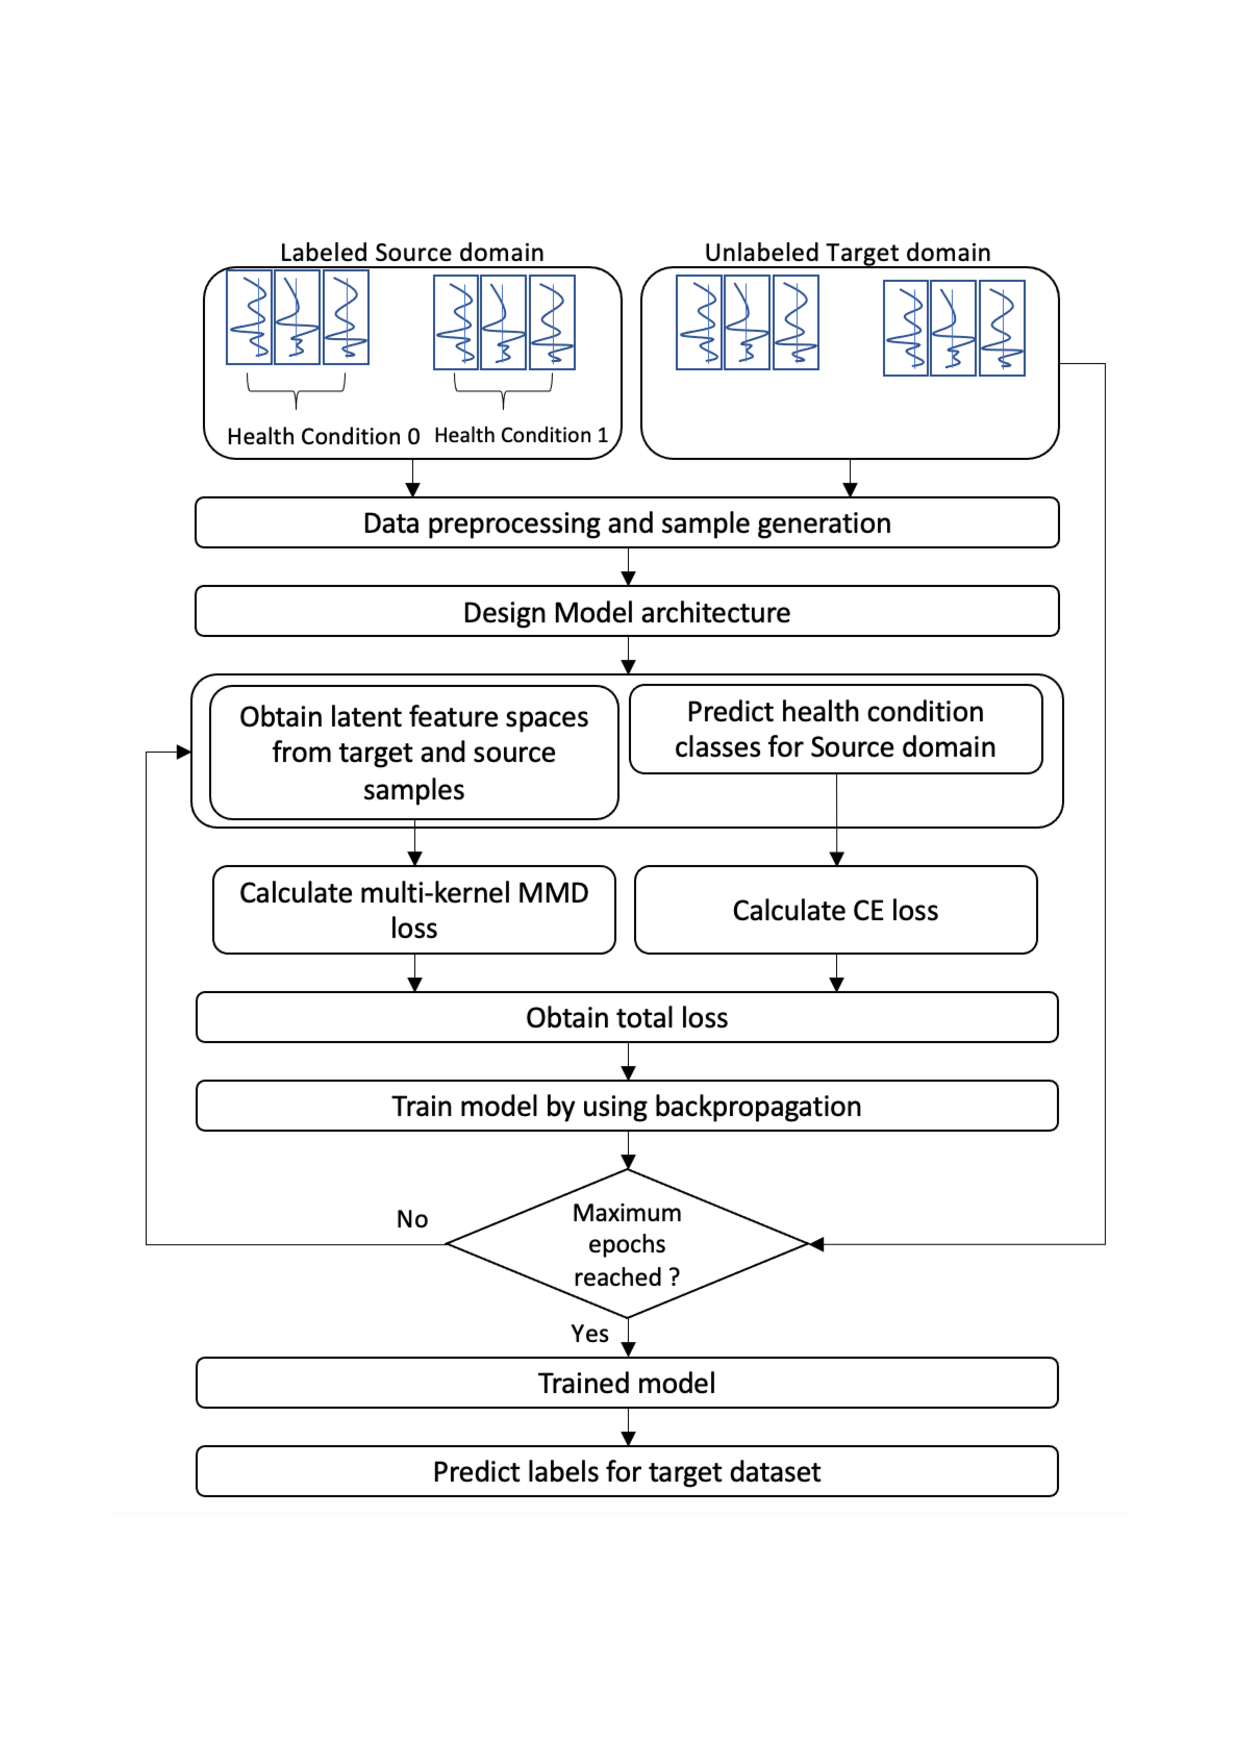
\includegraphics[width=0.8\textwidth]{training_process_mmd.pdf}
  \caption {Model Training} \label{fig:Training_Process_MMD}
\end{figure}


\chapter{Results}\label{chapter:results}
In the research community simplified synthetically generated datasets are quiet common for investigating underlying mechanisms and the applicability of different approaches for a given task. Of course, for the sake of completeness it is also necessary to test these approaches on the real-world task. Just if that is done properly one can estimate the robustness and therefore the actual benefit of the approach for the real-world task. In the following the results from different experiments on the dummy and the real-world dataset are described.

\section{Dummy Dataset}
Several experiments were performed on the dummy dataset to analyze the effects of the MMD loss in an easy and clear setting and to make first estimates about its applicability for PHM. The models used are the same as described in section \ref{sec:model}. The model in \ref{cnn_mmd_dummy} was optimized as explained in section \ref{sec:Proposed_training}. In the experiments of section \ref{sec:Balancing Cross-Entropy and MMD loss} and \ref{sec:Differences of labeled and unlabeled MMD loss} just one SGD optimizer with learning rate 0.01 in combination with a weighted average between the MMD and source cross-entropy loss was used.

\subsection{Influence of GAMMA Choice on the MMD Loss} \label{sec:Balancing Cross-Entropy and MMD loss}

In the following section, the sensitivity of the weighting factor GAMMA on the training is evaluated. The latent feature representation in FC2 for source and target domain is visualized in fig. \ref{fig:point_cloud_mmd}. The development of the MMD and cross entropy loss throughout the training is shown in fig. \ref{fig:learning_curves_influence_mmd_feature_extractor}.
\begin{itemize}
    \item \textbf{Small GAMMA}:
    When picking a very small GAMMA, the model is not able to generate a latent feature representation with a high compactness and separability between classes. Besides that, the class representations do not overlap well for the two domains. The domain discrepancy becomes especially visible for class 1. For this GAMMA choice, the source cross-entropy loss dominates the training. Instead of reducing the domain discrepancy, the model training focuses solely on predicting source samples correctly. The model is able to predict the source domain labels accurately but can not transfer that knowledge to the target domain. 
    \item \textbf{Medium GAMMA}:
    When the GAMMA is chosen carefully, the source cross-entropy and MMD loss can be reduced simultaneously. The class distributions in the latent feature space show increased compactness and separability for both domains. A trade-off is found, where the model is optimized to classify the source domain correctly and reducing the inter- and intra-class distances between source and target domain to minimize the domain discrepancy. Just in this case, the training profits from both losses equally. None of them dominates the training and thus prevents the combined training with multiple goals.
    \item \textbf{Big GAMMA}:
    When picking a very big GAMMA, the training is dominated by the MMD loss, such that the correct prediction of source domain samples becomes irrelevant. Since the target labels are unknown, the MMD loss is calculated between source and target samples of the same as well as different classes. Therefore, the MMD loss reduces the inter- and intra-class distance between the latent feature vectors of source and target domain. The separability of the classes is reduced. The optimization ends in a trivial solution, where all latent feature representations collapse at the same point or on a thin needle-like subspace. The model just reduces the distance between the samples of all classes and domains without aiming to solve the classification task.
\end{itemize}


\begin{figure}[H]
  \centering
  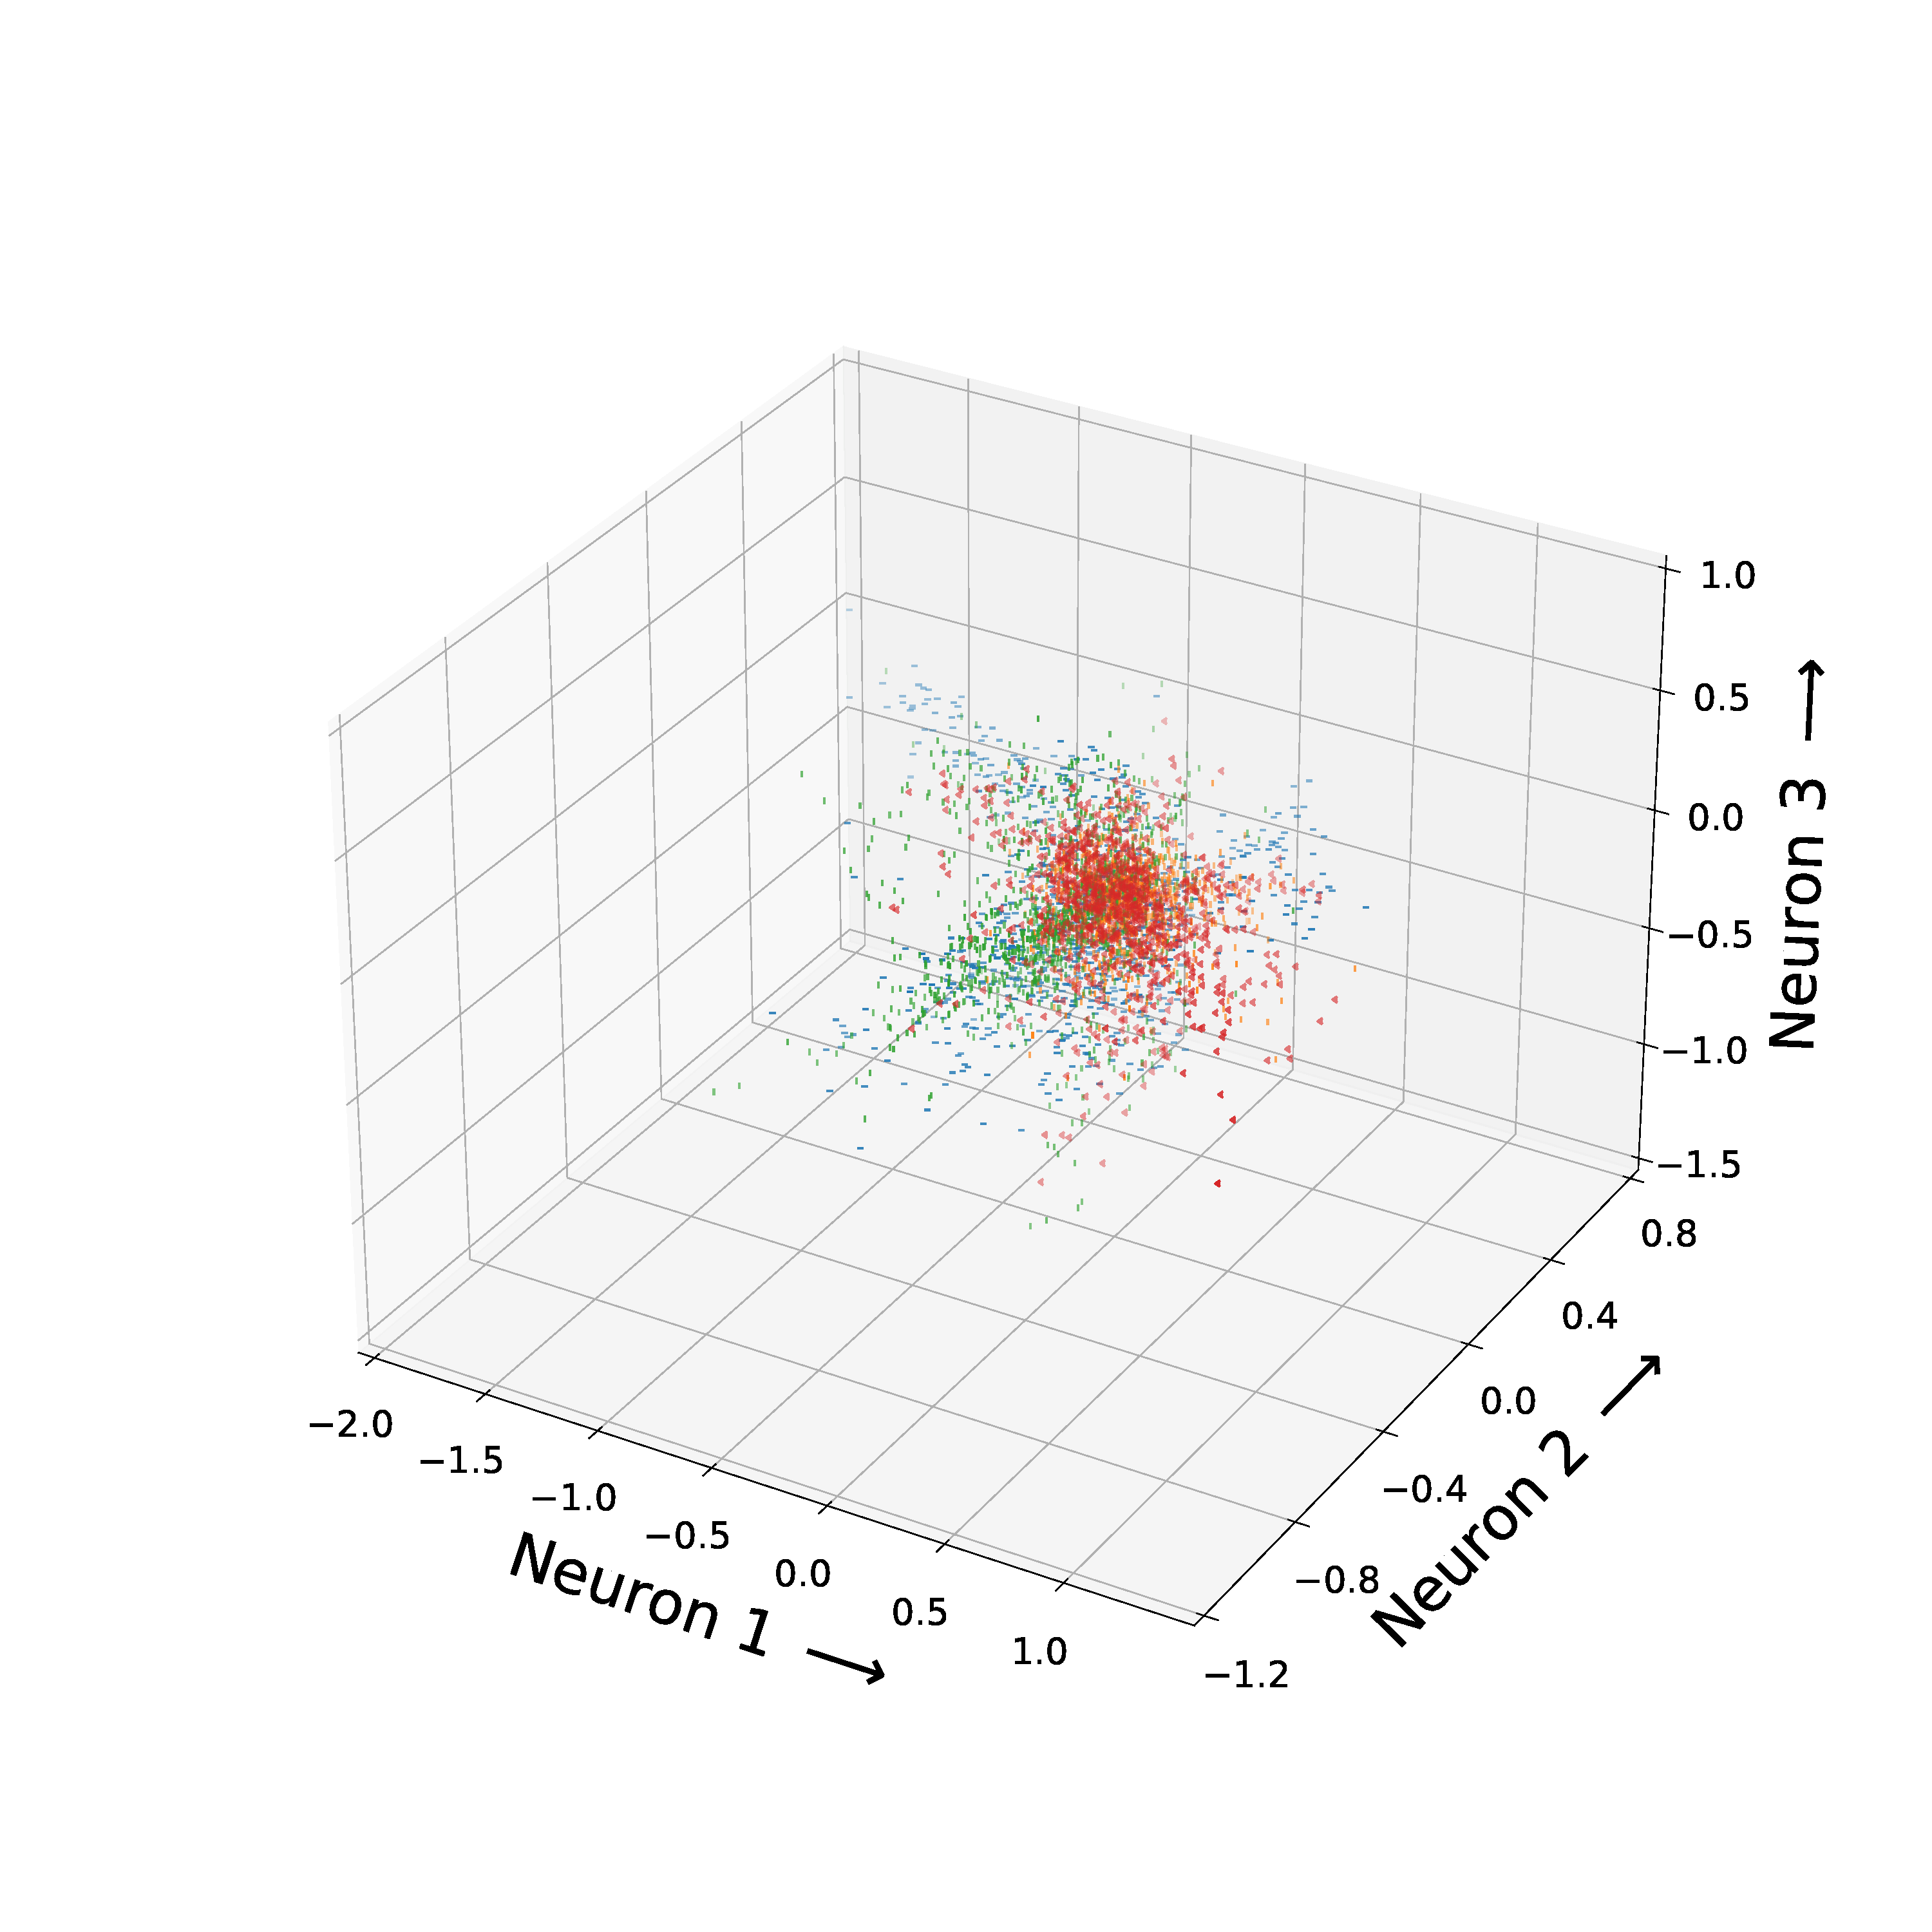
\includegraphics[width=.48\textwidth]{GAMMA_Influence_dummy_distribution/Dummy_distribution_0_GAMMA_0_001.pdf}
  \hspace{.4cm}
  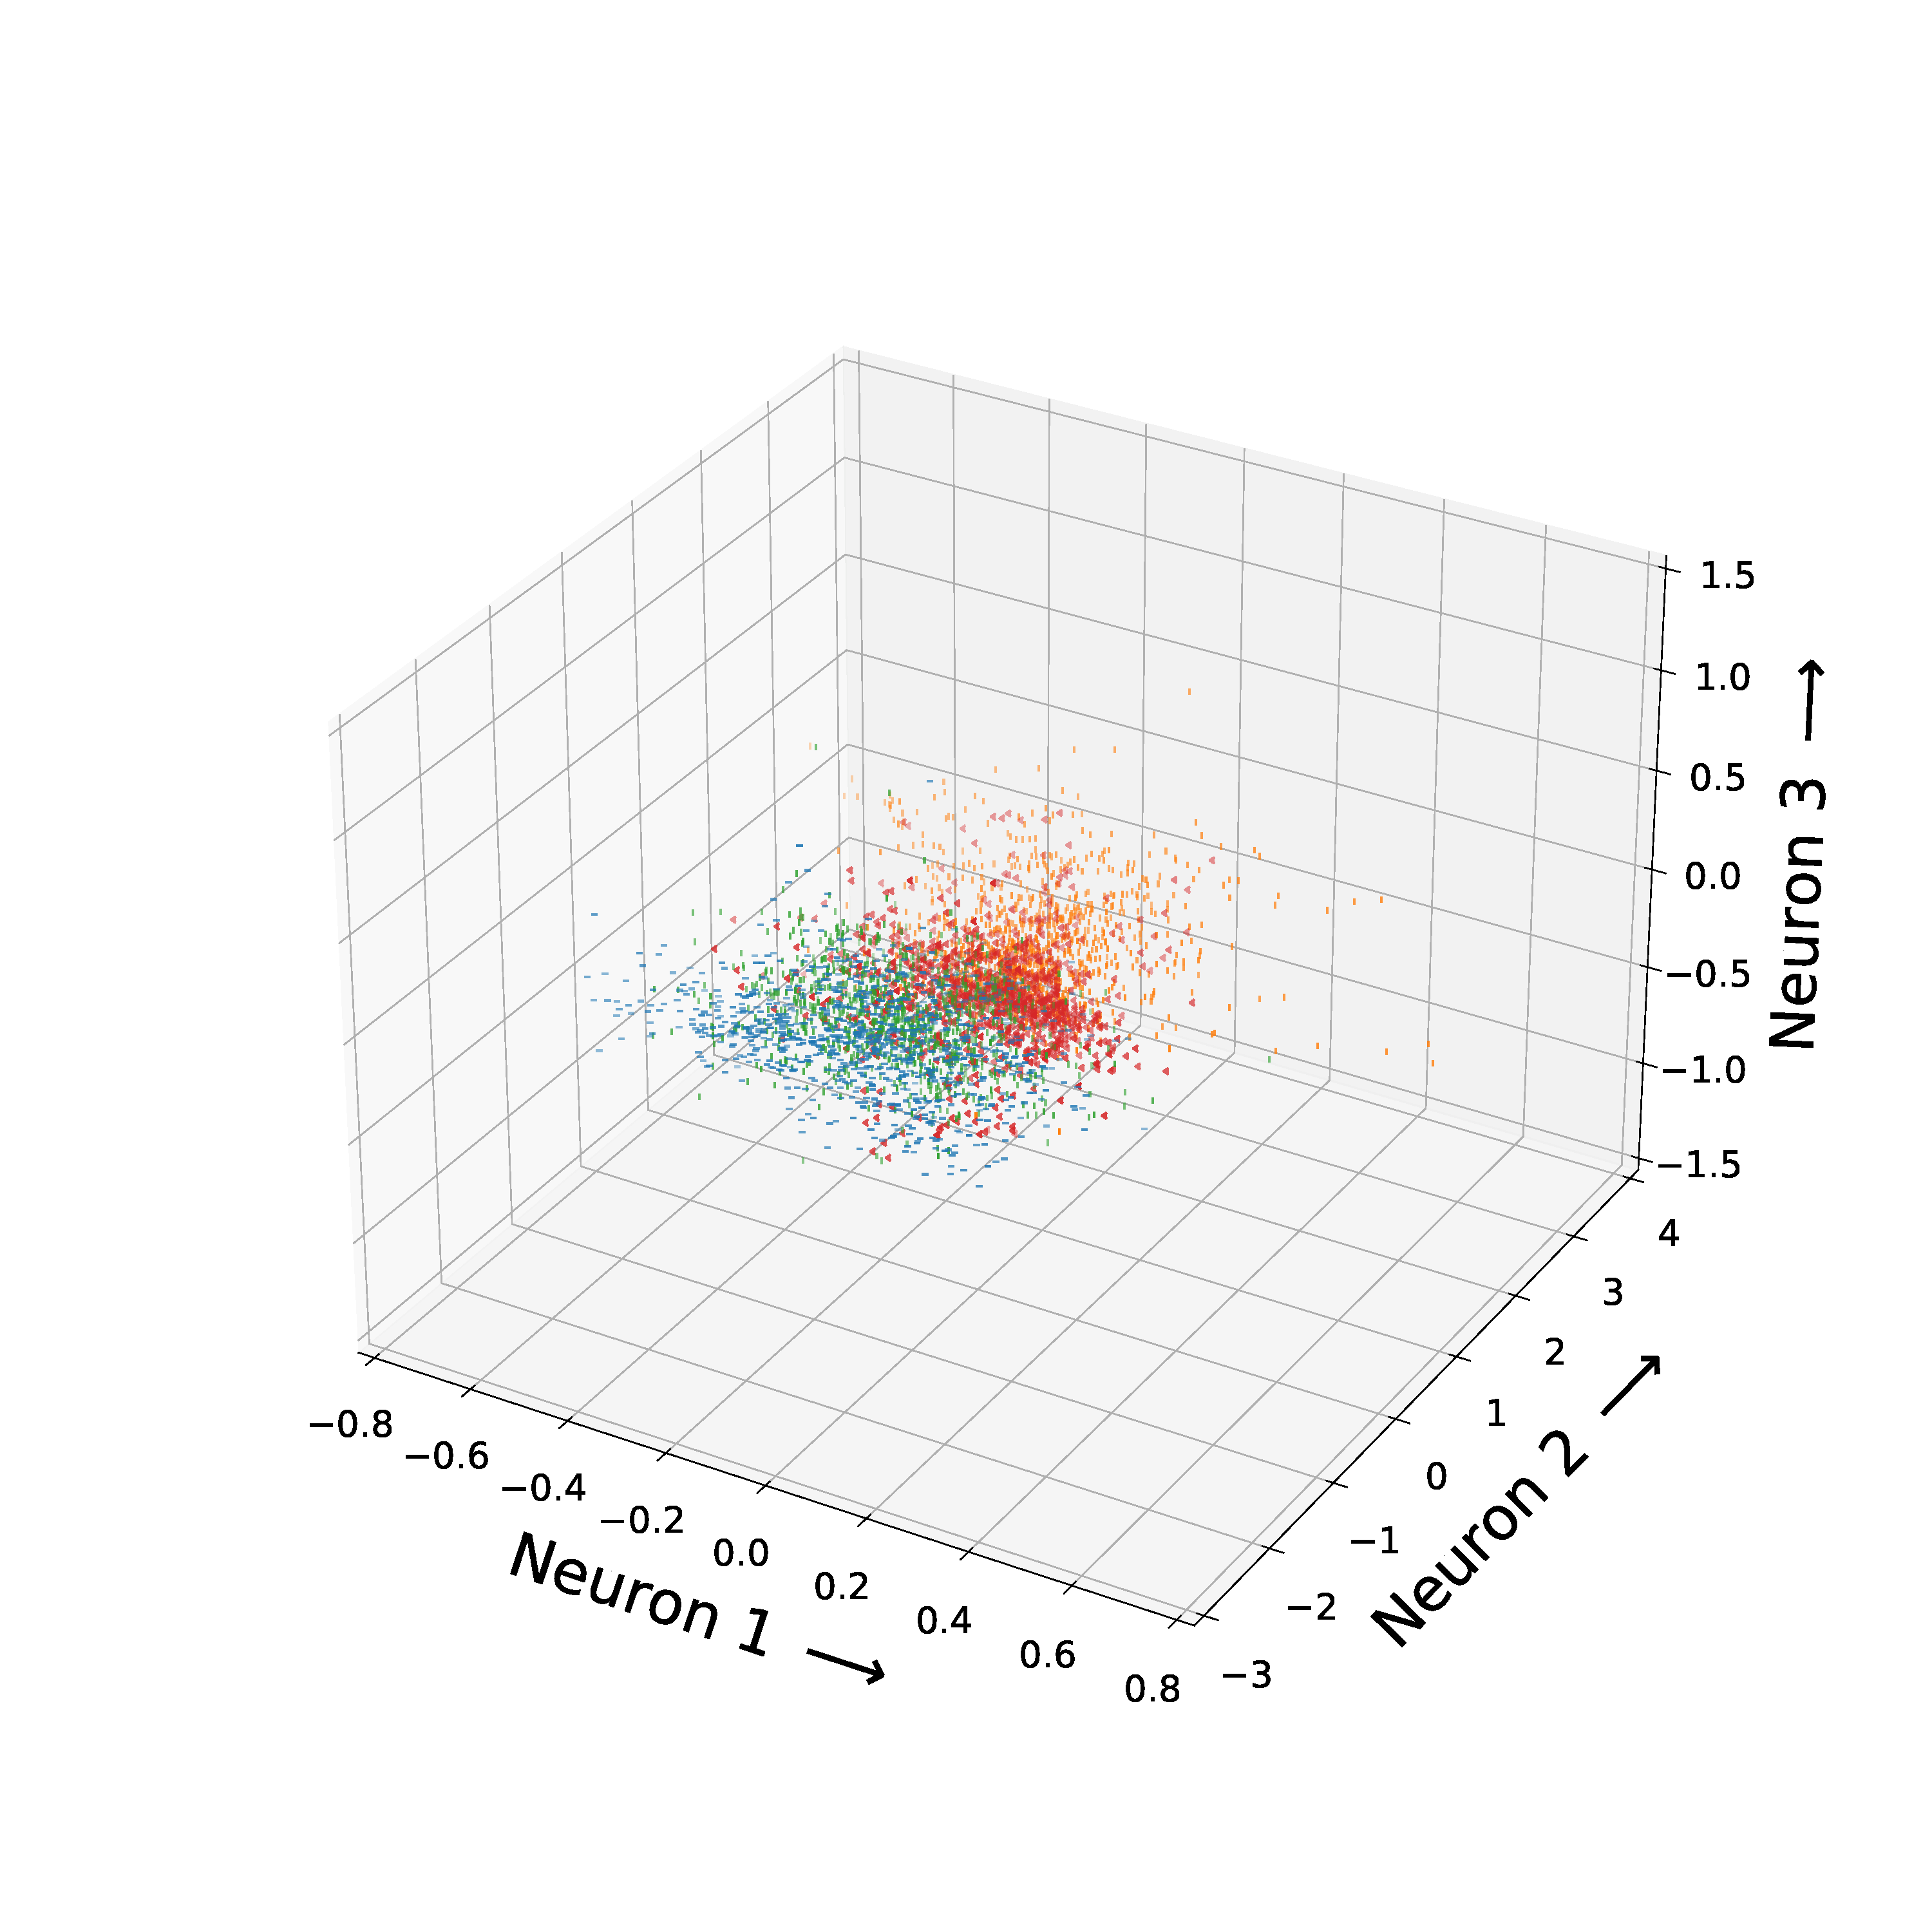
\includegraphics[width=.48\textwidth]{GAMMA_Influence_dummy_distribution/Dummy_distribution_8_GAMMA_0_001.pdf}

  \vspace{.1cm}

  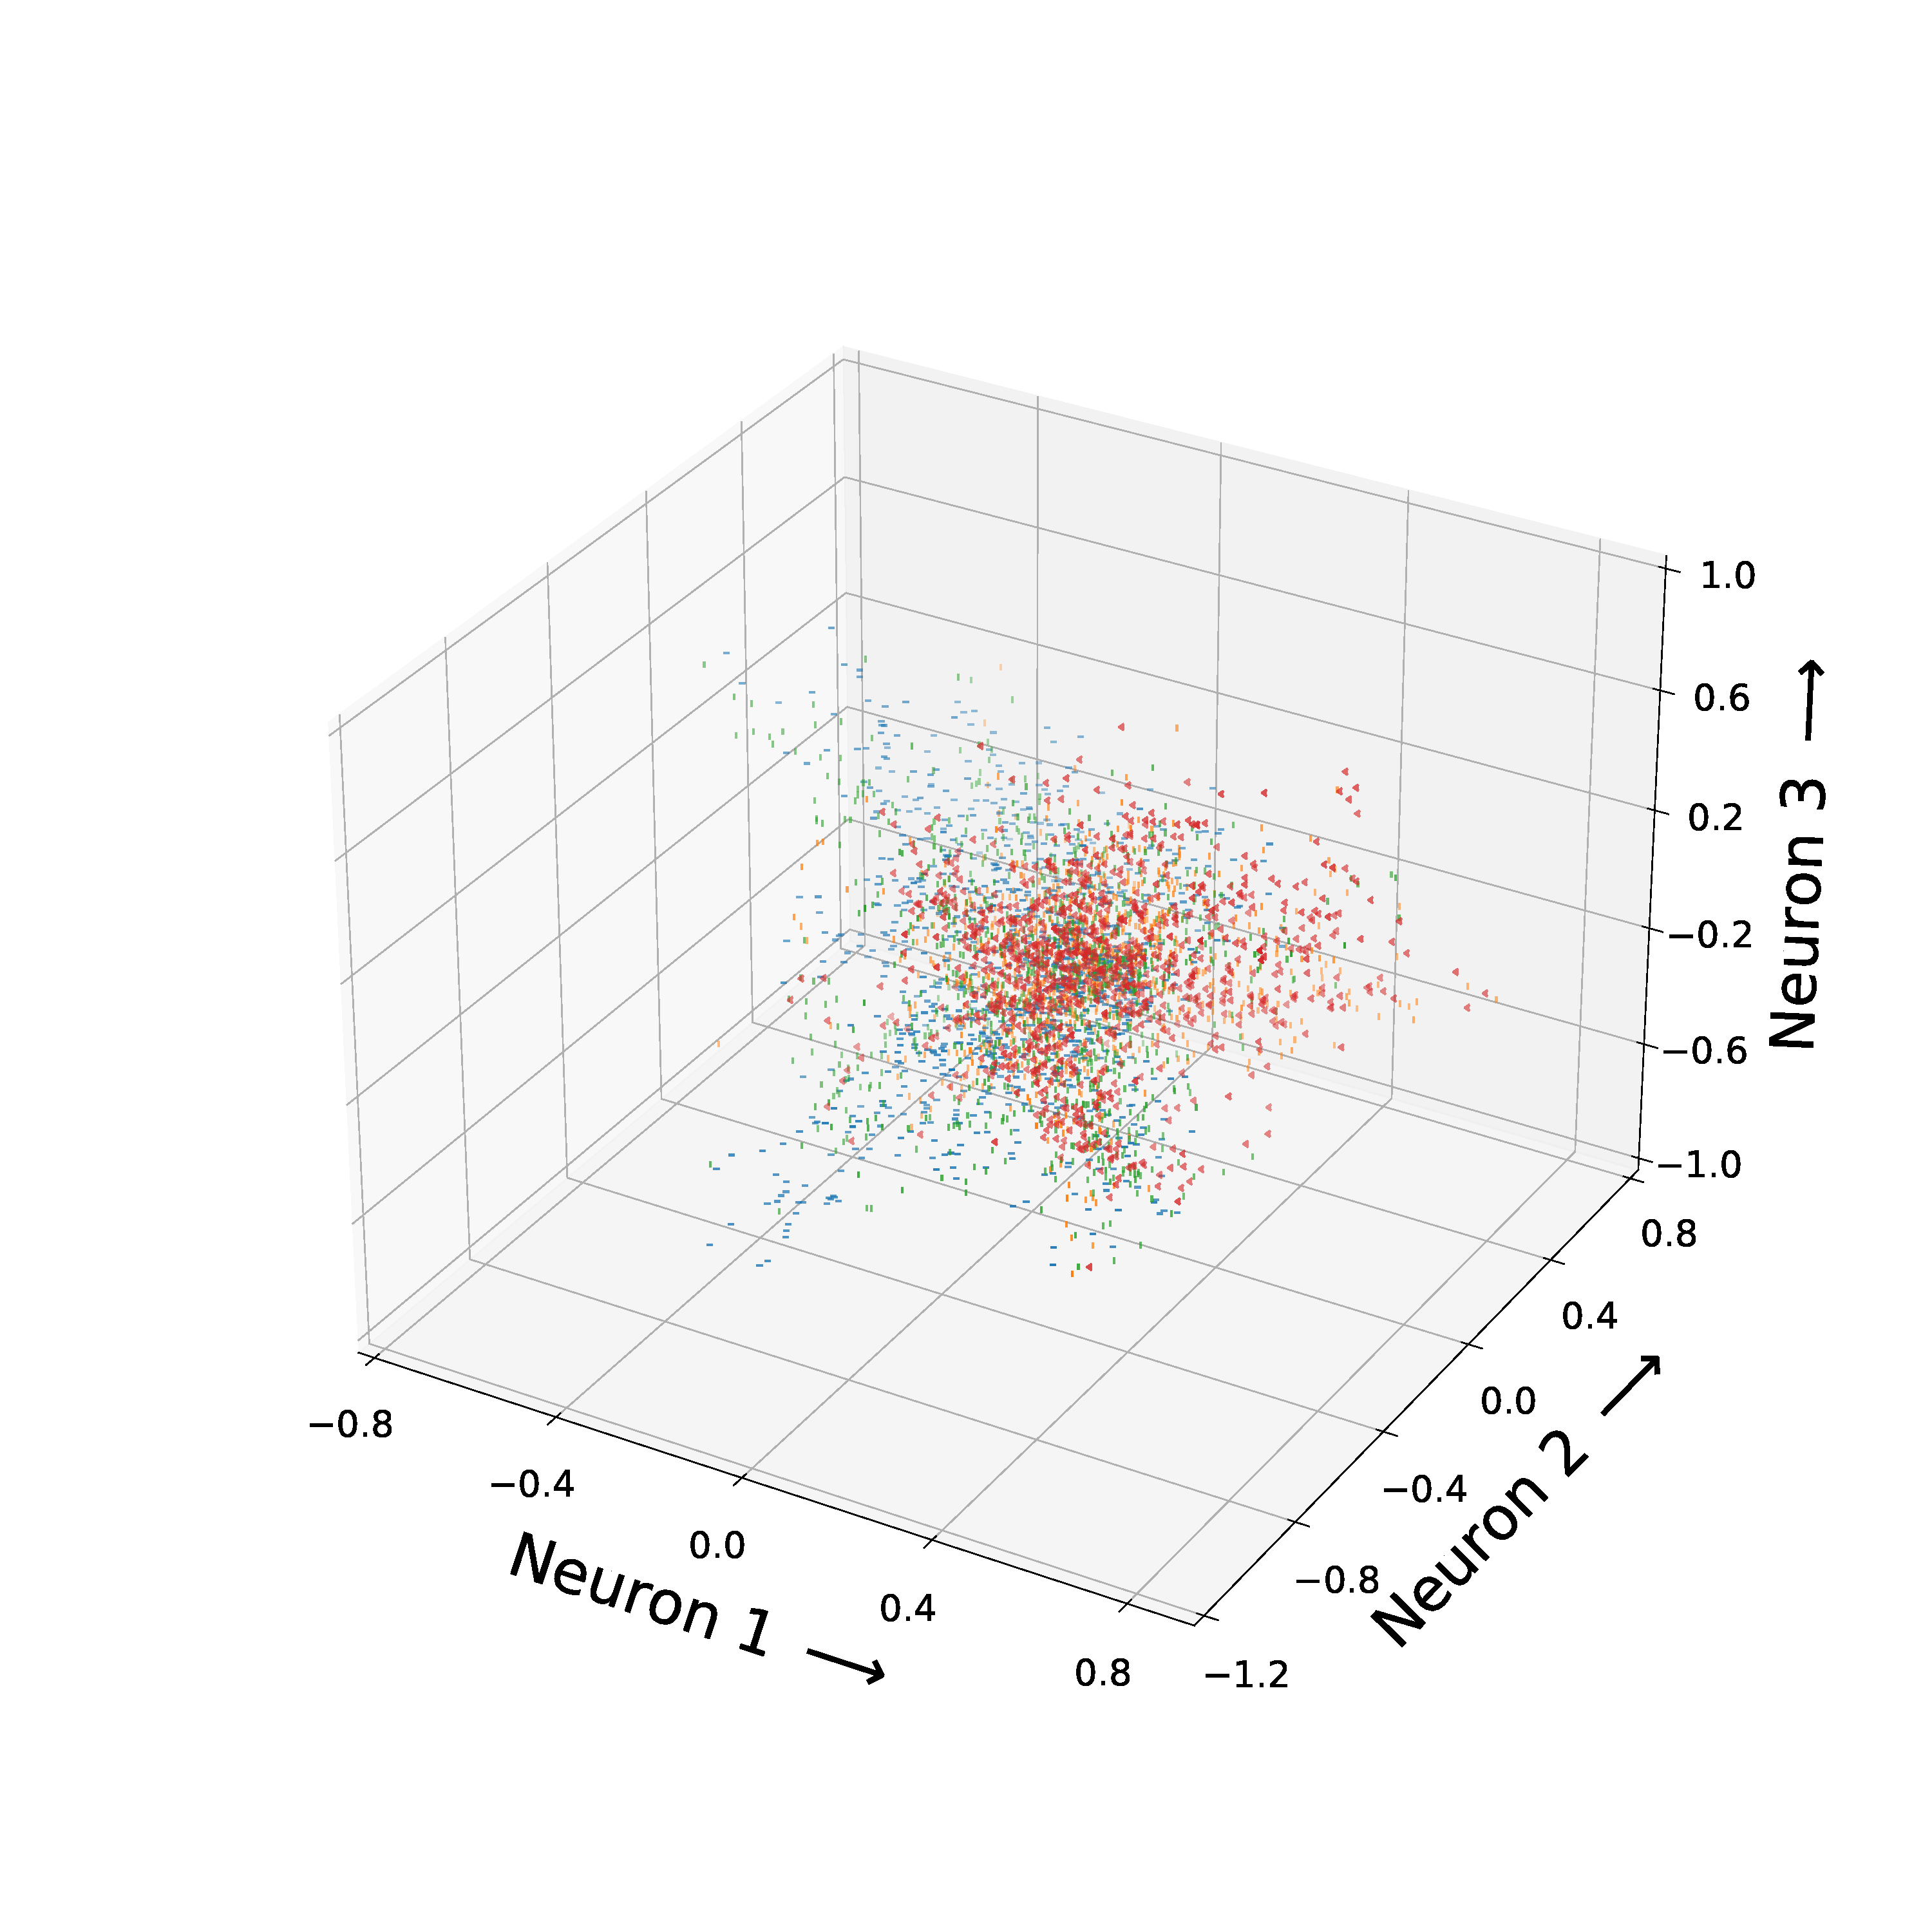
\includegraphics[width=.48\textwidth]{GAMMA_Influence_dummy_distribution/Dummy_distribution_0_GAMMA_0_1.pdf}
  \hspace{.4cm}
  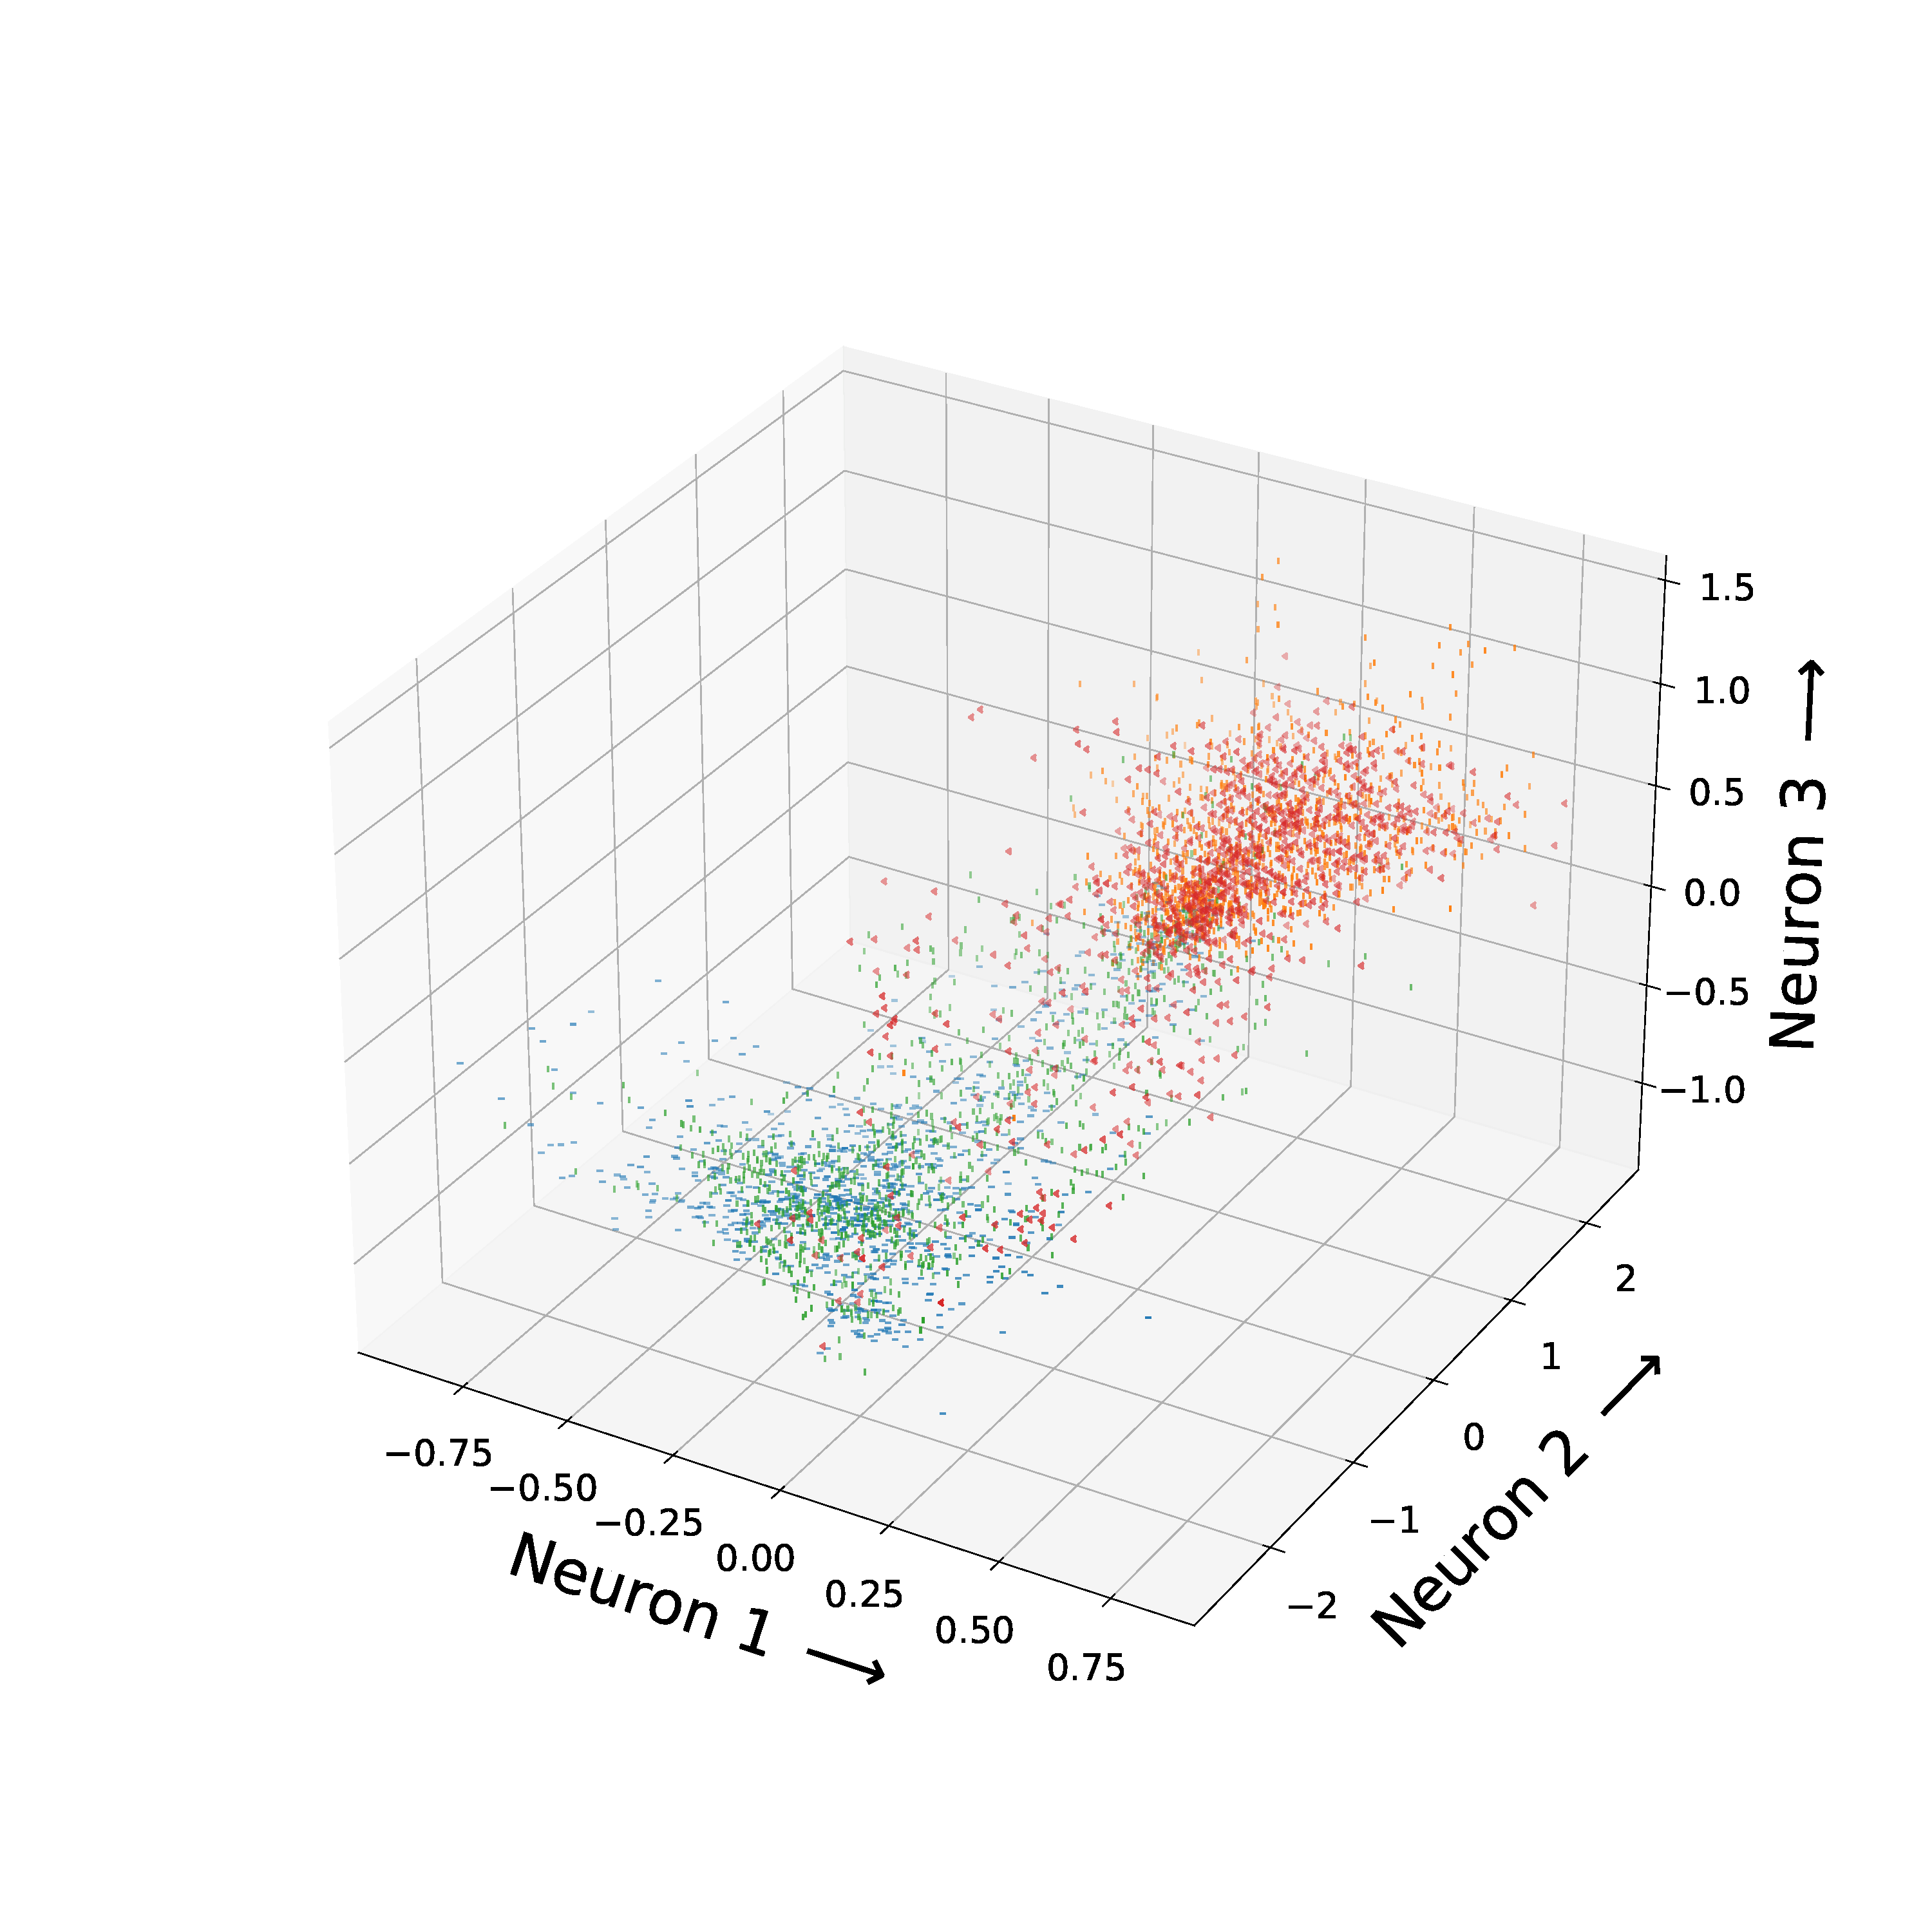
\includegraphics[width=.48\textwidth]{GAMMA_Influence_dummy_distribution/Dummy_distribution_8_GAMMA_0_1.pdf}

  \vspace{.1cm}

  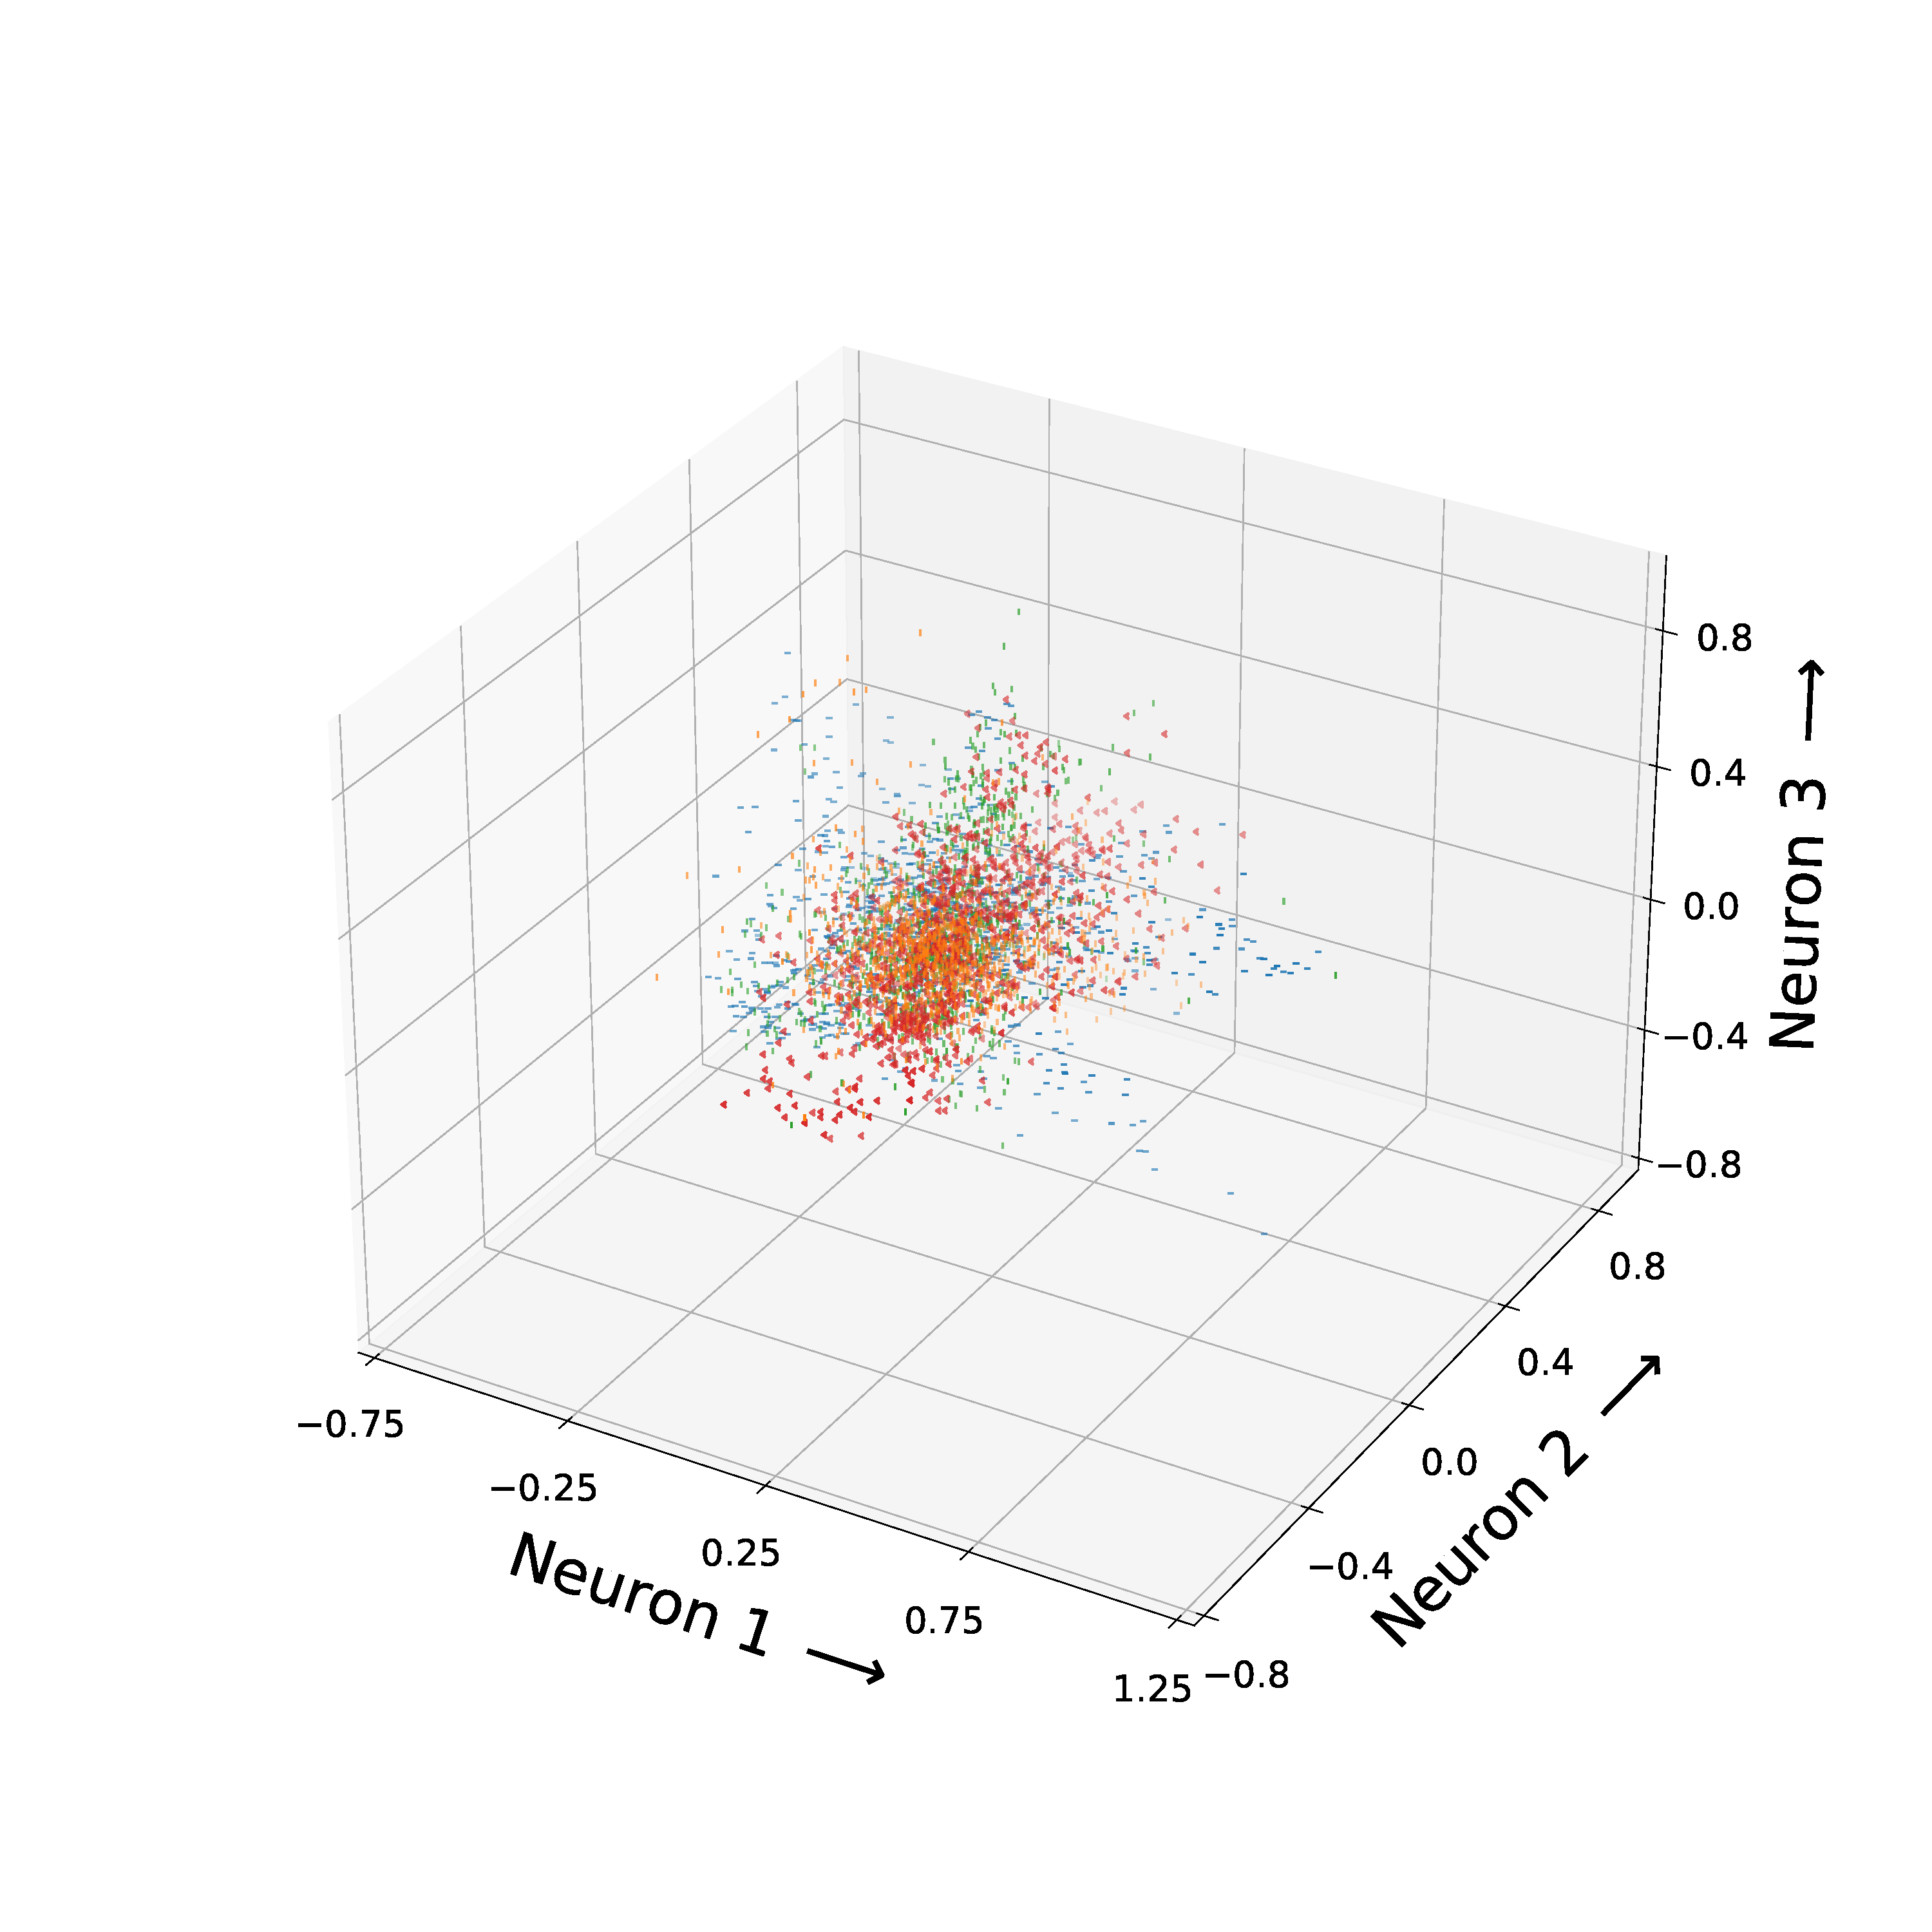
\includegraphics[width=.48\textwidth]{GAMMA_Influence_dummy_distribution/Dummy_distribution_0_GAMMA_20.pdf}
  \hspace{.4cm}
  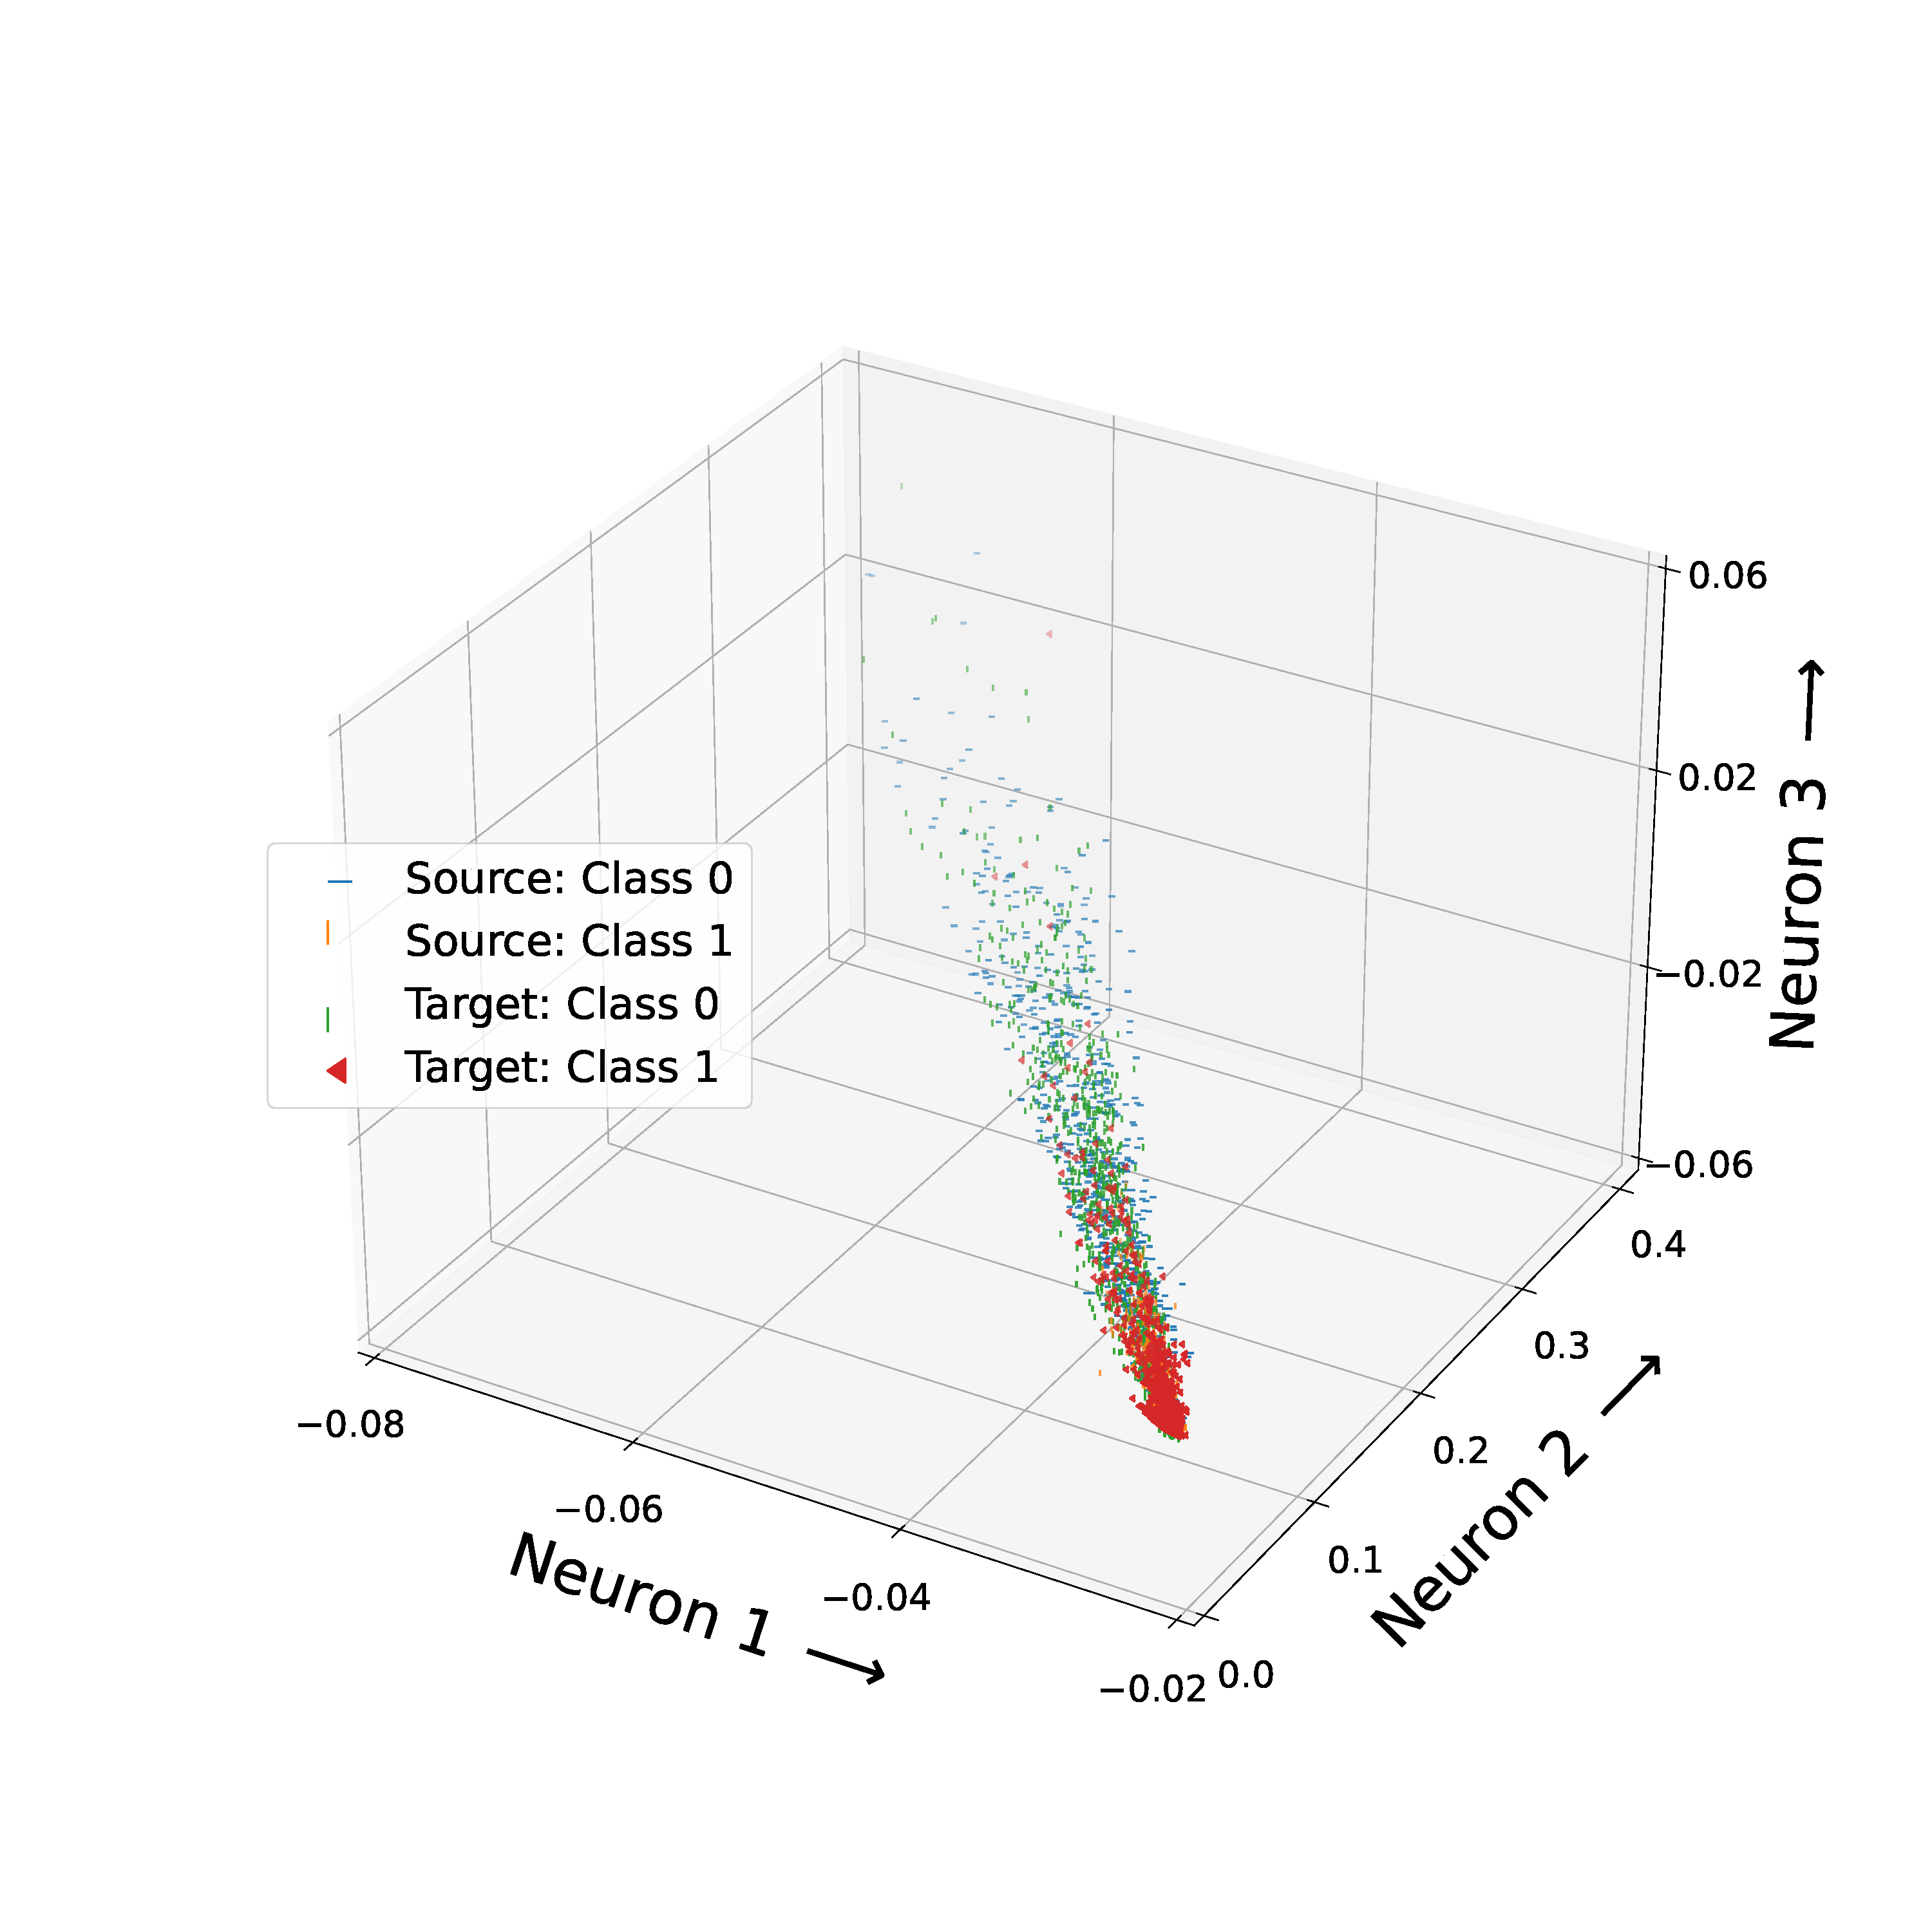
\includegraphics[width=.48\textwidth]{GAMMA_Influence_dummy_distribution/Dummy_distribution_8_GAMMA_20.pdf}
 

  \caption{Data distribution: Influence of GAMMA on Training, GAMMA = 0.05 (top), GAMMA = 0,4 (middle), GAMMA = 20 (bottom), Epoch = 0 (left) , Epoch = 8 (right)}
  \label{fig:point_cloud_mmd}
\end{figure}





\begin{figure}[H]
  \centering
  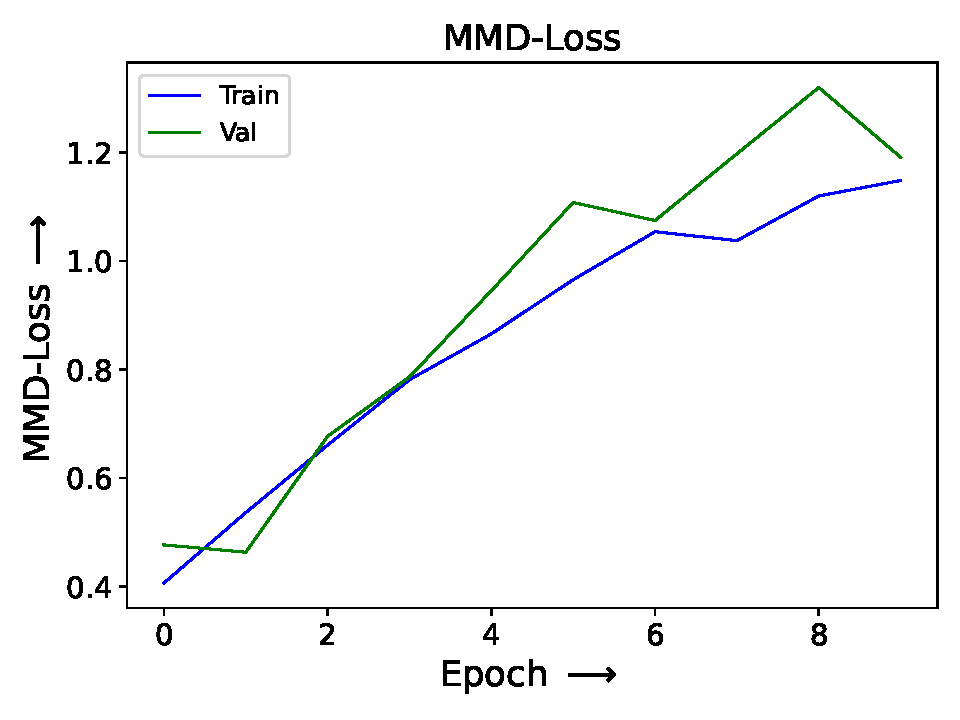
\includegraphics[width=.47\textwidth]{GAMMA_Influence_dummy_curve/MMD_Loss_GAMMA_0_001.pdf}
  \hspace{.3cm}
  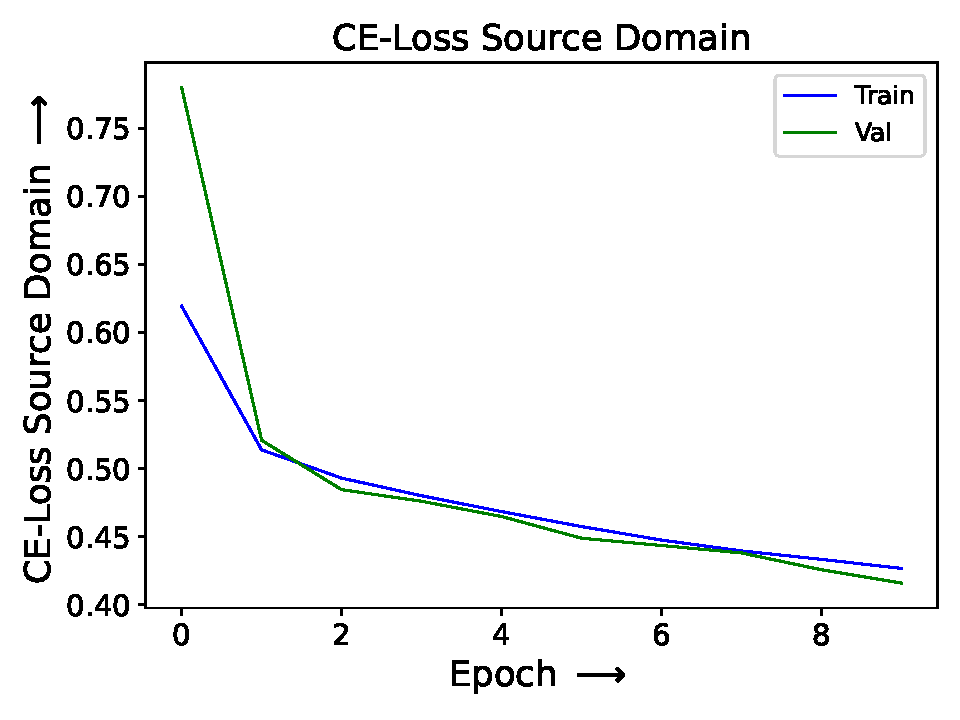
\includegraphics[width=.47\textwidth]{GAMMA_Influence_dummy_curve/CE_Loss_Source_Domain_GAMMA_0_001.pdf}

  \vspace{.1cm}

  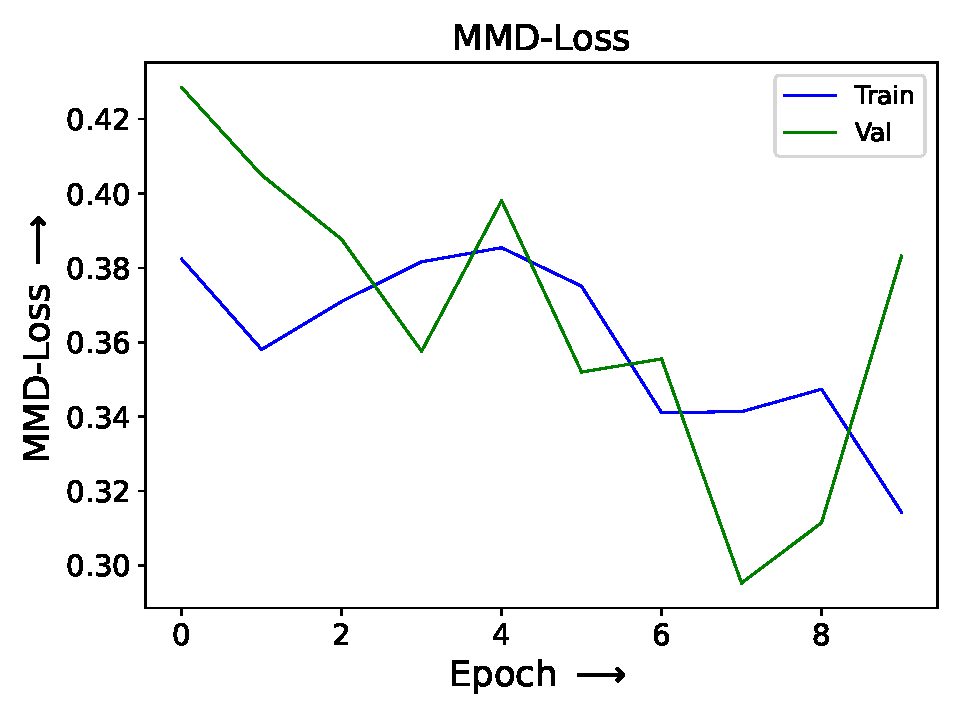
\includegraphics[width=.47\textwidth]{GAMMA_Influence_dummy_curve/MMD_Loss_GAMMA_0_1.pdf}
  \hspace{.3cm}
  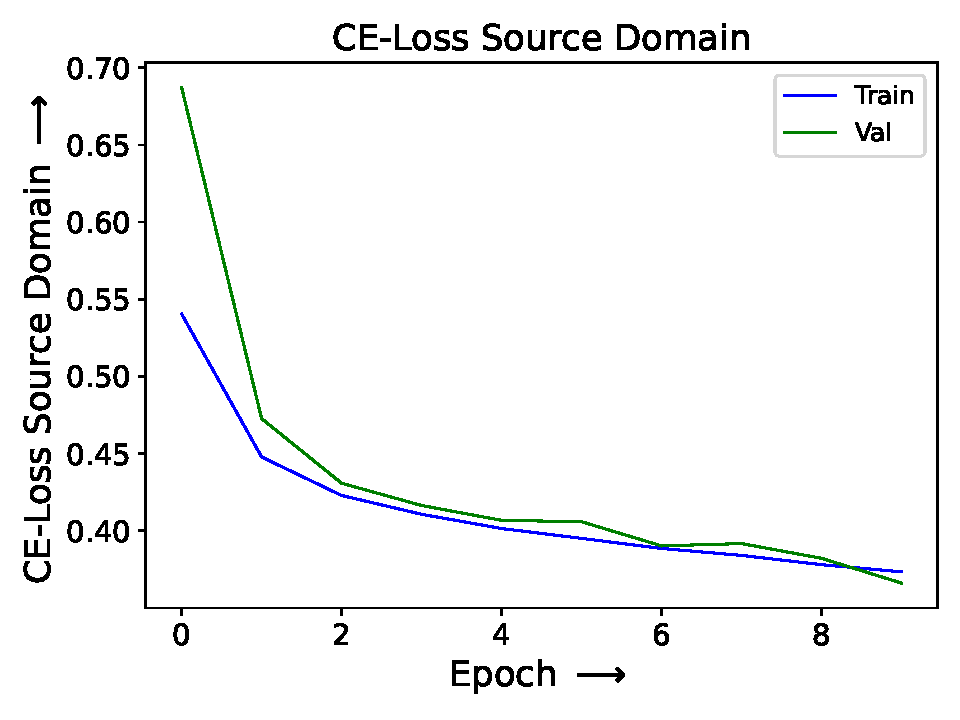
\includegraphics[width=.47\textwidth]{GAMMA_Influence_dummy_curve/CE_Loss_Source_Domain_GAMMA_0_1.pdf}

  \vspace{.1cm}

  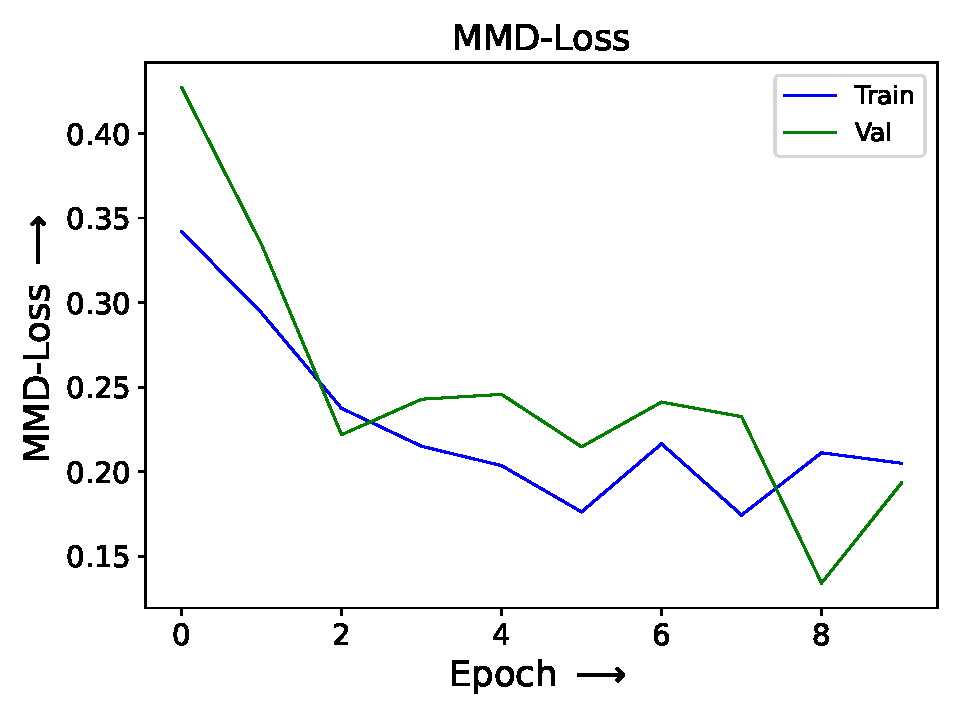
\includegraphics[width=.47\textwidth]{GAMMA_Influence_dummy_curve/MMD_Loss_GAMMA_20.pdf}
  \hspace{.1cm}
  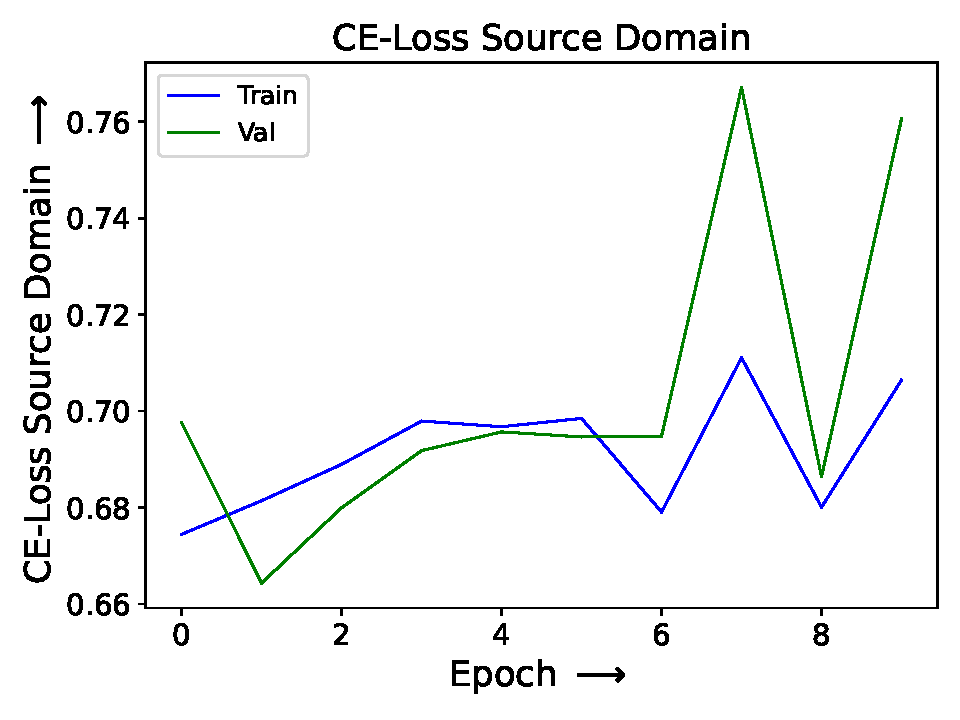
\includegraphics[width=.47\textwidth]{GAMMA_Influence_dummy_curve/CE_Loss_Source_Domain_GAMMA_20.pdf}

  \caption{MMD and Source CE-Loss: Influence of GAMMA on Training: GAMMA = 0.001 (top), GAMMA = 0.1 (middle), GAMMA = 20 (bottom), Epoch 0 (left), Epoch 8 (right)}
  \label{fig:learning_curves_influence_mmd_feature_extractor}
\end{figure}

\subsection{Labeled vs. Unlabeled MMD loss} \label{sec:Differences of labeled and unlabeled MMD loss}

The idea behind domain adaption is to aggregate knowledge while solving one problem and transferring that knowledge to another problem. For this reason, in domain adaption tasks the goal is to restrict the supervised learning solely on the source domain data. In the regular MMD loss, the target labels are unknown. Therefore, the intra- and inter-class distance between source and target samples is minimized equally. Obviously, this reduces the class separability in both domains. In the literature, domain adaption approaches which use a small amount of the target domain labels are known as "Few-shot transfer learning" \cite{WU2020}. Similarly, in this section the effect of including a few target labels into the training is analyzed. The cross-entropy loss is still restricted to the source domain. Solely the MMD loss is allowed to use target labels. The distance between source and target samples of similar and different classes can be calculated separately. The labeled MMD loss optimizes the model such, that the intra-class distance is maximized and the inter-class distance is minimized for both domains. This separate consideration of class distances allows a simultaneous improvement of class separability and compactness. Besides that, the training includes the source cross-entropy loss. The hyperparameters GAMMAIntraClass and GAMMAInterClass are used to balance the training scope of minimizing the inter-, maximizing the intra-class distance and increasing the source domain classification performance:

\begin{equation}
\begin{split}
    TotalMMDLoss = GAMMAIntraClass * MMDLossIntraClass\\ + GAMMAInterClass * MMDLossInterClass + CELoss
\end{split}
\end{equation}

 The MMD loss which includes the target labels is named "labeled MMD loss" and otherwise "unlabeled MMD loss". Again, fig. \ref{fig:point_cloud_labeled_unlabeled_mmd} visualizes the latent feature representation in FC2. Throughout the training, the labeled MMD loss is able to reduce the domain discrepancy while increasing the separability and compactness of the classes in both domains. This simplifies the classification problem and makes the model optimization less prone to find a trivial solution, in which the latent feature representation of all samples collapse at one point or a needle-like subspace. In this experiment, 20\% of target labels were used in labeled MMD loss.
\begin{figure}[H]
  \centering
  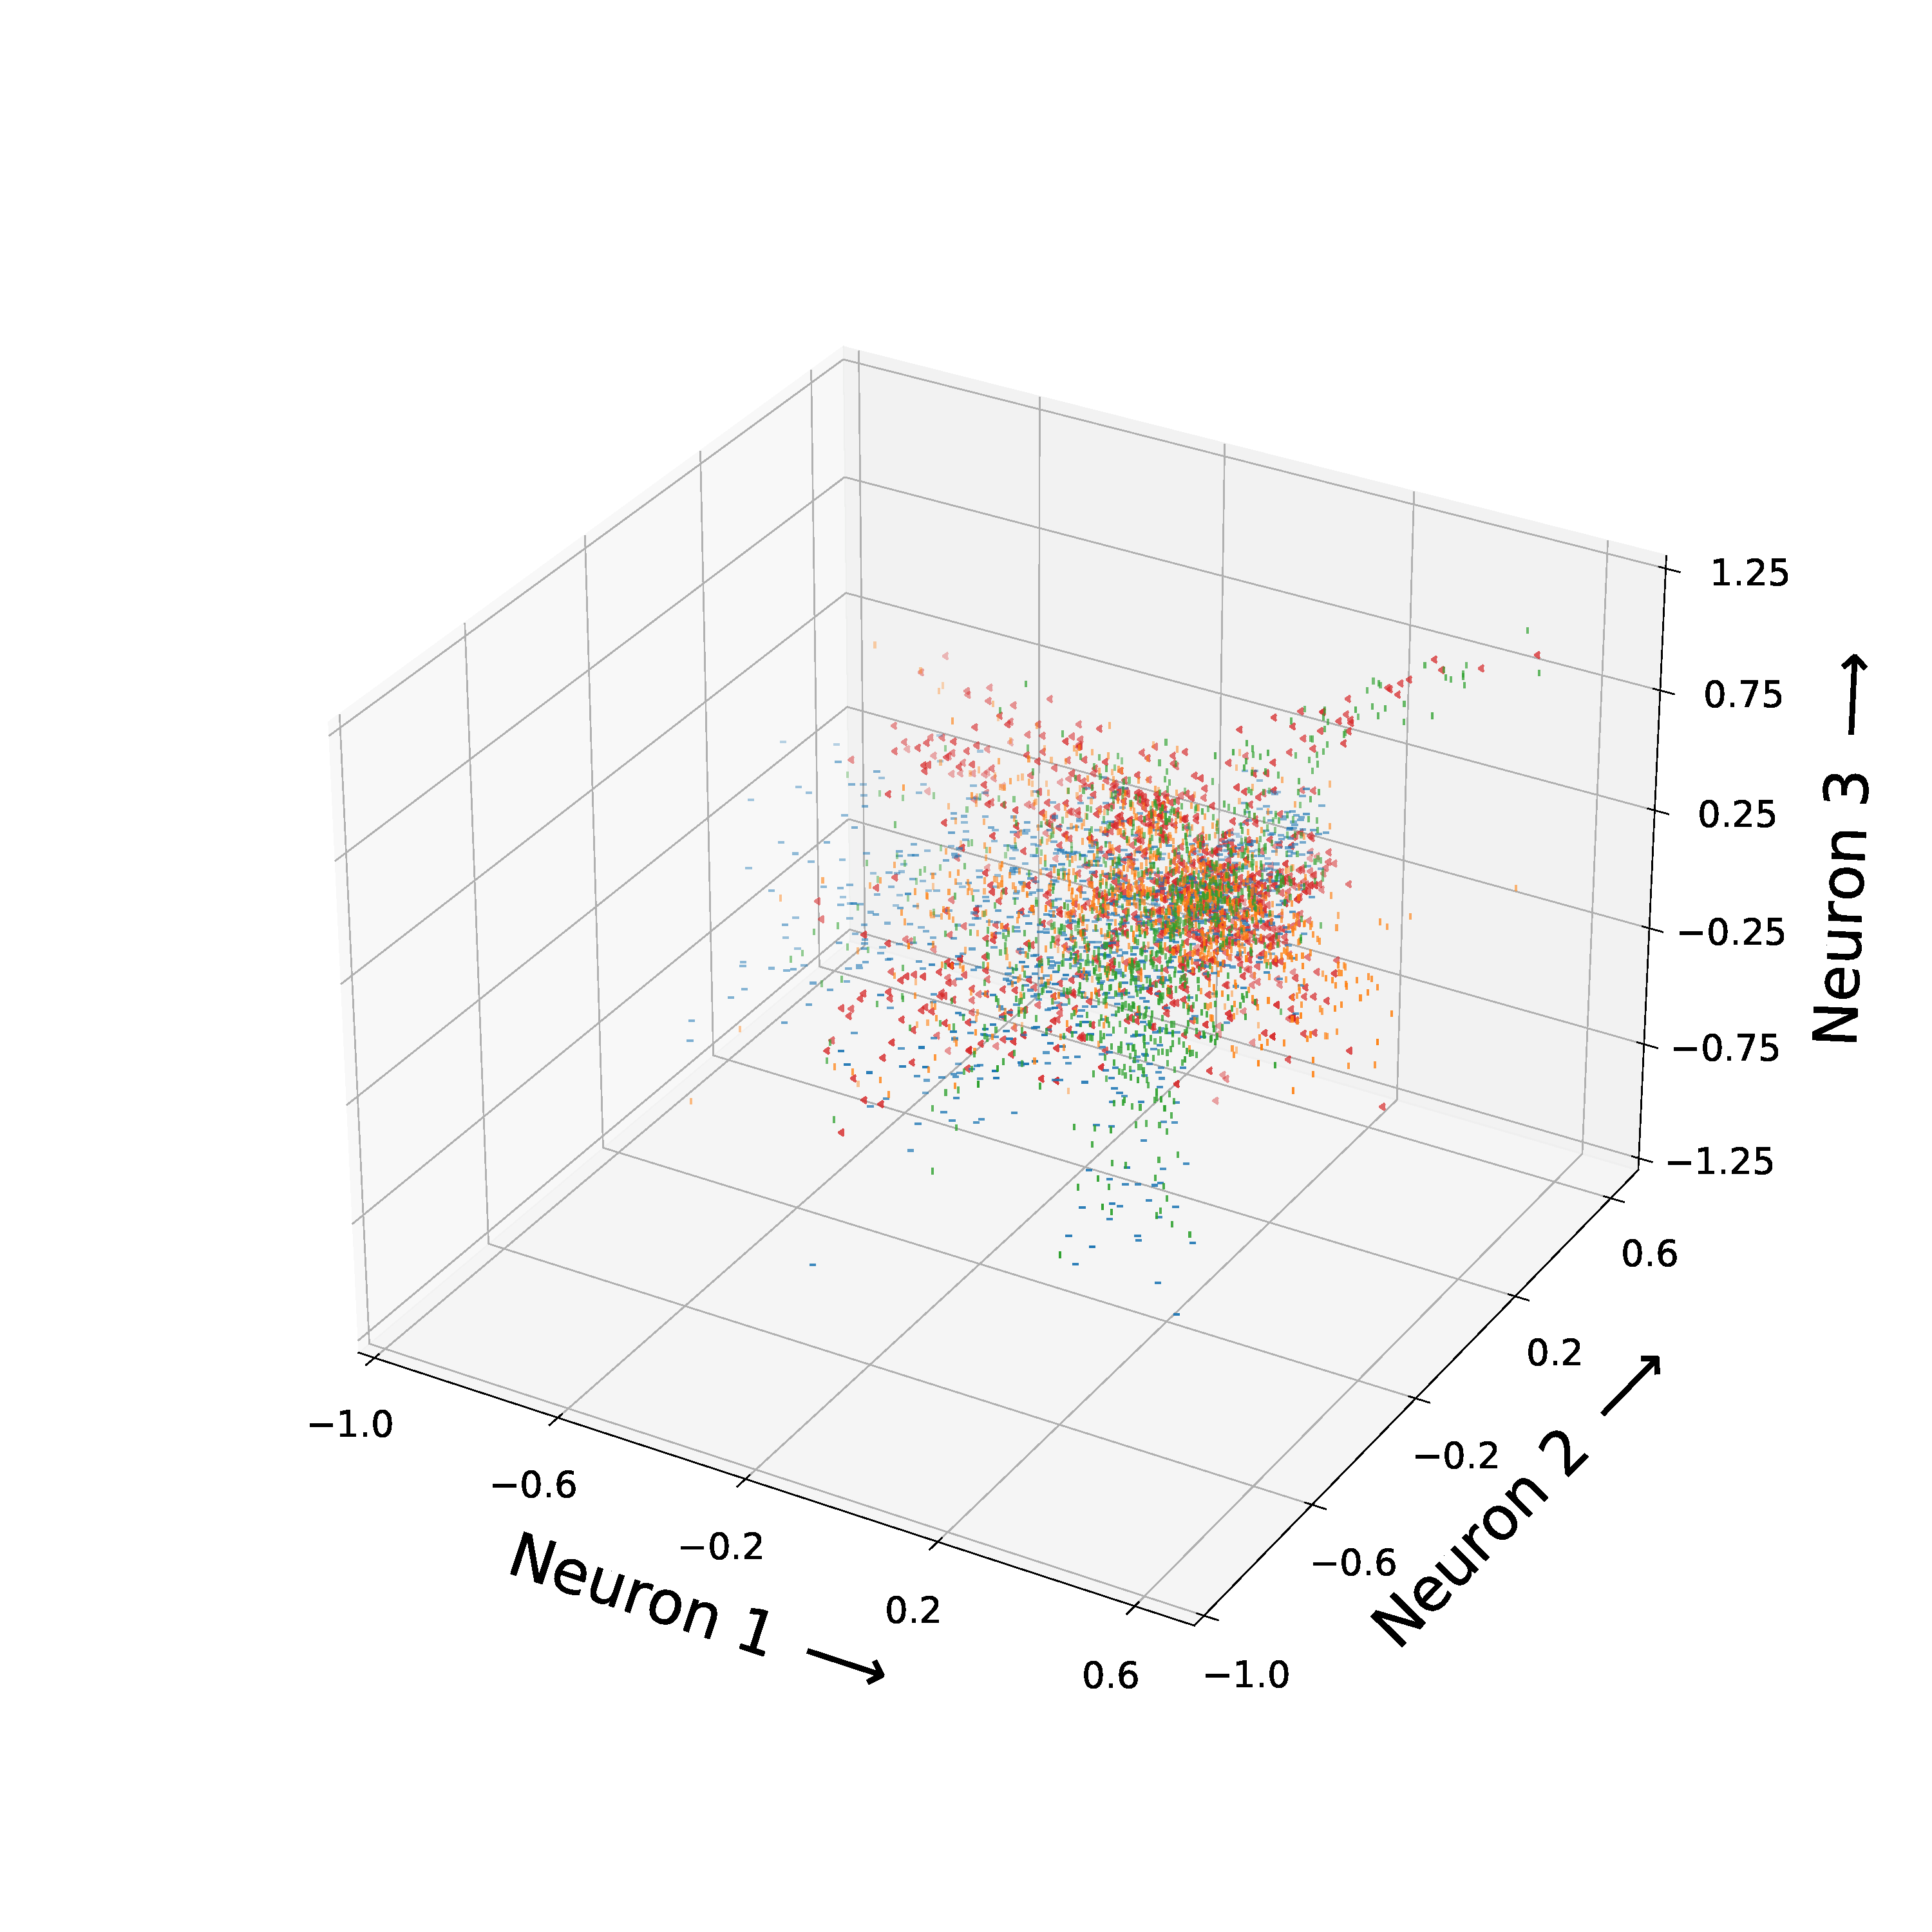
\includegraphics[width=.44\textwidth]{labeled_vs_unlabeled_point_cloud/data_distribution_labeled_mmd_0.pdf}
  \hspace{.4cm}
  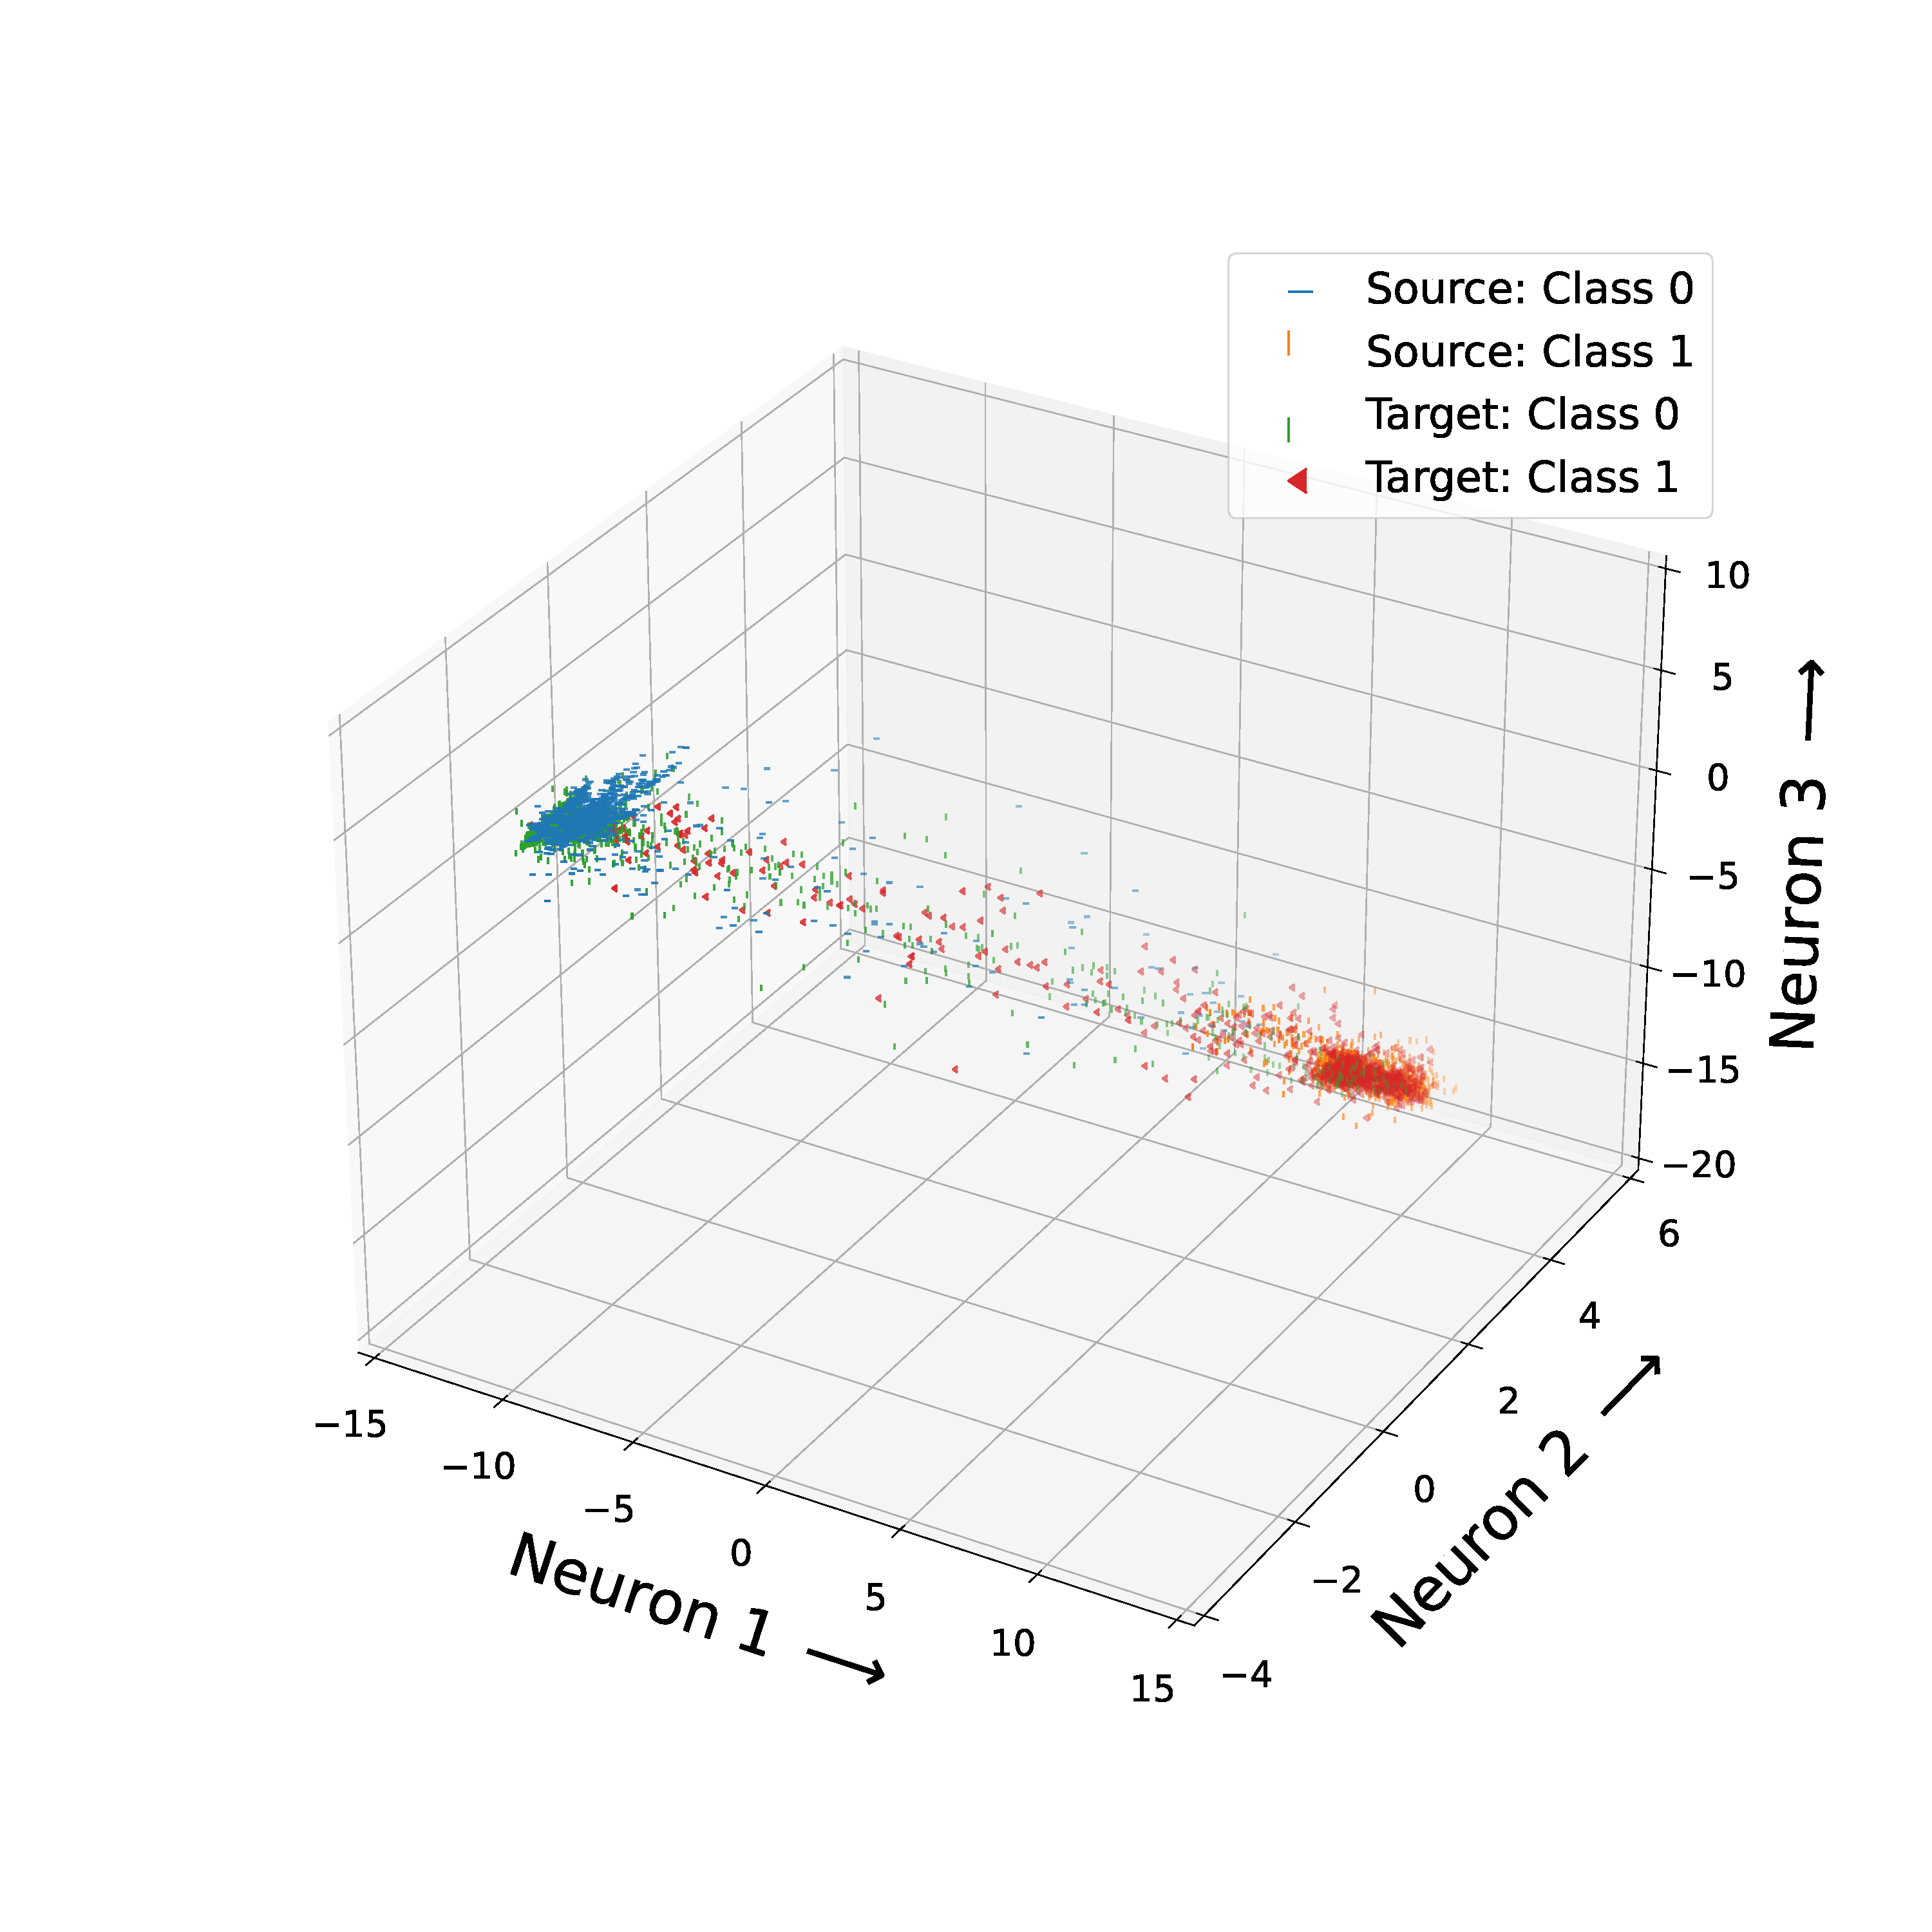
\includegraphics[width=.44\textwidth]{labeled_vs_unlabeled_point_cloud/data_distribution_labeled_mmd_6.pdf}

  \vspace{.1cm}

  \includegraphics[width=.44\textwidth]{labeled_vs_unlabeled_point_cloud/data_distribution_regular_mmd_0.pdf}
  \hspace{.4cm}
  \includegraphics[width=.44\textwidth]{labeled_vs_unlabeled_point_cloud/data_distribution_regular_mmd_6.pdf}
  
  \caption{Data Distribution: Labeled MMD (top) vs. Unlabeled MMD (bottom): Epoch 0 (left) vs. Epoch 6 (right)}
  \label{fig:point_cloud_labeled_unlabeled_mmd}
\end{figure}

\subsection{Influence of Latent Feature Space Choice on the MMD Loss}
\label{cnn_mmd_dummy}
This section analyzes the influence of applying the MMD loss in different latent feature maps of the CNN and classifier. The "regular FC MMD" loss calculates the source and target discrepancy from the three latent feature maps in the classifier (flattened output of CNN, FC1, FC2). The "regular FC + CNN MMD" loss additionally considers the feature maps of the three convolutional layers in the CNN (Conv 1, Conv 2 and Conv 3). The accuracy, the source cross-entropy and MMD loss during the training process are shown in fig. \ref{fig:accuracy_cnn_and_no_cnn_mmd} and fig. \ref{fig:loss_cnn_and_no_cnn_mmd}. The accuracies in source and target domain are higher when including the CNN feature maps into the MMD loss. Besides that, including the CNN feature maps in the MMD loss increases the stability of the training. The losses, as well as the accuracies, converge faster and smoother.

\begin{figure}[H]
  \centering
  \includegraphics[width=.47\textwidth]{plots_CNN_MMD/Accuracy_Source_Domain_CNN_MMD.pdf}
  \hspace{.3cm}
  \includegraphics[width=.47\textwidth]{plots_CNN_MMD/Accuracy_Source_Domain_FC_MMD.pdf}

  \vspace{.1cm}

  \includegraphics[width=.47\textwidth]{plots_CNN_MMD/Accuracy_Target_Domain_CNN_MMD.pdf}
  \hspace{.3cm}
  \includegraphics[width=.47\textwidth]{plots_CNN_MMD/Accuracy_Target_Domain_FC_MMD.pdf}

  \caption{Source and Target Accuracy: MMD in CNN (left), MMD in FC (right)}
  \label{fig:accuracy_cnn_and_no_cnn_mmd}
\end{figure}

\begin{figure}[H]
  \centering
  \includegraphics[width=.47\textwidth]{plots_CNN_MMD/CE_Loss_Source_Domain_CNN_MMD.pdf}
  \hspace{.3cm}
  \includegraphics[width=.47\textwidth]{plots_CNN_MMD/CE_Loss_Source_Domain_FC_MMD.pdf}

  \vspace{.1cm}

  \includegraphics[width=.47\textwidth]{plots_CNN_MMD/MMD_Loss_CNN_MMD.pdf}
  \hspace{.1cm}
  \includegraphics[width=.48\textwidth]{plots_CNN_MMD/MMD_Loss_FC_MMD.pdf}

  \caption{MMD and CE-Loss: MMD in CNN (left), MMD in FC (right)}
  \label{fig:loss_cnn_and_no_cnn_mmd}
\end{figure}

By passing data through the model, features with varying levels of abstraction are extracted. Supervising the domain discrepancy in feature maps of different abstraction levels seems reasonable. Generally, shallow layers in neural network extract more global and deeper more task-specific features. Deeper layers often suffer from stronger domain-dependencies. Since each layer in a neural network influences subsequent layers, it makes sense to apply the MMD loss early in the network. Reducing the domain discrepancy in shallow layers makes the network extract more domain-invariant features in all following layers as well. Especially in challenging tasks with strong domain discrepancies, it is reasonable to intervene early. Reducing the domain discrepancy just in the final layers of the model leads to a less stable and smooth optimizations. Potentially, the MMD and source cross-entropy loss tend to be more contradicting when applied in these layers. The two training goals, which seem to work against each other, make the optimization more fluctuating. During the optimization, different strong local minima coming from one of the two losses might be found. The model performance sometimes breaks down after some stable epochs of constant training. One has to remember calculating the regular FC + CNN MMD loss is quite expansive since the feature maps extracted from the convolutional layers are complex and high-dimensional.



\section{Real-World Dataset}
In the following section the performance of different MMD-based domain adaption models are evaluated on the real-world ball screw dataset. The goal of this chapter is to evaluate the benefits and problems of the presented approach for PHM on industrial machines. All presented models have the same architecture but differ in their optimization processes. Different GAMMA and MMD layer choices were evaluated. The performance of each model is compared with the base-line model, which does not use any MMD loss during training. In the following table the MMD layer choices of the different models are presented:

\begin {table}[H]
\centering

\begin{tabular}{llllllll}
  \toprule
  Model          & Conv1 & Conv2 & Conv3 & FC1 & FC2 & FC3 \\
  \midrule
  
\vspace{.5cm}

 \parbox[t]{0mm}{\multirow{1}{*}{\rotatebox[origin=c]{90}{\thead{BASE- \\ LINE}}}} & - & - & - & - & - & -\\
 
\vspace{.5cm}

 \parbox[t]{0mm}{\multirow{1}{*}{\rotatebox[origin=c]{90}{\thead{FULL \\ MMD}}}} & \checkmark & \checkmark & - & \checkmark & \checkmark & \checkmark\\
 
\vspace{.5cm}

 \parbox[t]{0mm}{\multirow{1}{*}{\rotatebox[origin=c]{90}{\thead{FC \\ MMD}}}} & - & - & - & \checkmark & \checkmark & \checkmark\\
 
\vspace{.5cm}

 \parbox[t]{0mm}{\multirow{1}{*}{\rotatebox[origin=c]{90}{\thead{CNN \\ MMD}}}} & \checkmark & \checkmark & \checkmark & - & - & -\\

 
  \bottomrule
\end{tabular}

\caption {MMD layer choice of presented models} \label{tab:MMD_layer_choice} 
\end {table}

Similarly to the dummy dataset, the influence of GAMMA and the MMD layer choice on the PHM performance are examined in the chapter \ref{ch:Influence_GAMMA_real_dataset} and \ref{ch:Influence_Layer_real_dataset}. Since the previously presented labeled MMD loss uses target labels, which all other models do not, the labeled MMD loss models were not included in the evaluation on the real data. To achieve good comparability just models with equal training conditions are considered. In the chapter \ref{ch:PHM_performance} the actual performance of different models for the PHM task on ball screw drives is evaluated by the target accuracy on the test data.  


\begin{comment}
In the following section the performance of different MMD-based domain adaption approaches are evaluated on the real-world ball screw dataset. The model used for this evaluation is presented in fig. \ref{fig:model_real_data}. From the 49 features in the dataset just three (\verb|'C:x_bottom'|, \verb|'C:y_bottom'|, \verb|'C:z_bottom'|) are used. For this reasons three sequences of length 1024 are fed into the CNN.

\begin{figure}[H]
  \centering
  \includegraphics[width=1.1\textwidth]{model_real_data}
  \caption {MMD Model for Real Dataset} \label{fig:model_real_data}
\end{figure}


On the real machine dataset the three approaches regular FC + CNN MMD loss,  regular FC MMD and no MMD loss are evaluated. The accuracies on the source and target domain are visualized in fig. \ref{fig:accuracy_real_world}. In each figure three curves are presented representing different phases of the training. During the MMD Loss phase the whole model consisting of CNN and classifier are optimized with a weighted average of MMD and cross entropy loss. In the CE-Loss phase just the classifier is optimized according to a cross-entropy loss. During both phases an ADAM optimizer with a learning rate of 1e-2, beta1 of 0.9 and beta2 of 0.99 is used . In the val phase the model is evaluated. Before the training the data is split for these three phases accordingly (MMD-Loss: 60\%, CE-Loss: 20\%, Val: 20\%). Therefore all experiments follow a proper train validation split. It becomes obvious that the accuracies achieved on the validation set of the target domain were able to be increased with about 10\% by using the two MMD variations. The MMD and cross entropy loss seems to be decreased more smoothly when including CNN features into the MMD loss for the optimization of the model. Also the accuracy achieved on the target validation set achieved the regular FC + CNN MMD loss beat the one achieved with the regular FC MMD loss. Without using any MMD loss the model performance on the target domain could be increased by just around 2\%. When using the regular FC MMD loss sometimes the performance of the model breaks down  little bit. Often times this can be seen in the accuracy of the target and source domain. An example for this phenomena can be seen in fig. \ref{fig:accuracy_real_world} when looking at the accuracies of regular FC MMD (middle). In epoch ~27 the accuracy breaks down on the target and source domain. Especially during the combined training with the MMD and cross entropy loss this effect becomes especially obvious. Like mentioned in previous chapters this shows that when not including the latent features of the CNN in the MMD loss the cross entropy and MMD loss seem to work against each other, which makes the optimization less stable.

\begin{figure}[H]
  \centering
  \includegraphics[width=1.1\textwidth]{accuracy_real_world}
  \caption {Source and Target Accuracies for model training with Regular FC + CNN MMD loss (left), Regular FC MMD (middle) and No MMD loss (right)} \label{fig:accuracy_real_world}
\end{figure}


\begin{figure}[H]
  \centering
  \includegraphics[width=1.1\textwidth]{loss_real_world}
  \caption {Loss for model training with Regular FC + CNN MMD loss (left), Regular FC MMD (middle) and No MMD loss} \label{fig:loss_real_world}
\end{figure}


In fig. the development of the source domain cross entropy MMD loss is shown. It can be seen, that the hyperparameter GAMMA was picked well, such that the MMD as well as the source cross entropy loss were able to be reduced smoothly throughout the trainings process. 


Unfortunately the MMD loss could just minimize the domain discrepancy by a little. The domain discrepancy problem couldn't be solved completely. Still the idea of the MMD loss becomes more clear in the experiments. Also the positive effect of the MMD loss for the training is obvious. For the complex multi-dimensional dataset the MMD loss is probably not sophisticated enough to detect and effectively fight the domain discrepancy.
\end{comment}






\subsection{Influence of GAMMA Choice on the PHM Performance}\label{ch:Influence_GAMMA_real_dataset}

In the following three models are trained with a full MMD loss and different GAMMAs (0.05, 0.4, 20). The models were trained on the  D:P mech./X signal for 100 epochs. Similarly to the dummy dataset, the model training is very sensitive to the GAMMA choice. Just when GAMMA is chosen correctly, the source cross entropy and MMD loss can be reduced simultaneously. Both training goals, reducing the domain discrepancy in the models hidden layer and classifying the source domain samples correctly, can be pursued in parallel. Fig. \ref{fig:distribution_GAMMA_influence_real_data} shows the latent feature representation of the source and target domain samples of both classes in FC2. The left column shows the data distribution before training and the right one after 100 epochs. Applying the MMD loss with GAMMA of 0.05 increases the compactness of the classes from both domains. Due to the higher compactness also corresponding classes from the two domains overlap more, which reduces the domain discrepancy. From the plots it is hard to make a statement about the separability of the classes. When picking a GAMMA of 0.05 the structure of the data distribution seems to be clearer and smoother. This rises the assumption, that finding a separation between the classes of both domains might be easier. Anyhow, the actual performance gains due to the MMD loss is discussed later on. Generally, the MMD loss enables  domain invariant features which allows transferring knowledge learned from one domain to the other. If the MMD loss becomes too dominant also noise and unimportant information are transferred between the domains. Then the structure of the source and target domain data is destroyed, which makes the classification task impossible. When increasing GAMMA to 1, this scenario occurs. The feature representations of the samples from all classes and domains collapse at a small latent feature subspace.

\begin{figure}[htp]
  \centering
  \includegraphics[width=.47\textwidth]{GAMMA_Influence_real_data/P_mech_X_data_distribution_0_GAMMA_0_0.pdf}
  \hspace{.4cm}
  \includegraphics[width=.47\textwidth]{GAMMA_Influence_real_data/P_mech_X_data_distribution_40_GAMMA_0_0.pdf}

  \vspace{.1cm}

  \includegraphics[width=.47\textwidth]{GAMMA_Influence_real_data/P_mech_X_data_distribution_0_GAMMA_0_05.pdf}
  \hspace{.4cm}
  \includegraphics[width=.47\textwidth]{GAMMA_Influence_real_data/P_mech_X_data_distribution_40_GAMMA_0_05.pdf}

  \vspace{.1cm}

  \includegraphics[width=.47\textwidth]{GAMMA_Influence_real_data/P_mech_X_data_distribution_0_GAMMA_1_0.pdf}
  \hspace{.4cm}
  \includegraphics[width=.47\textwidth]{GAMMA_Influence_real_data/P_mech_X_data_distribution_40_GAMMA_1_0.pdf}

  \vspace{.1cm}

  \caption{Data  distribution:  Influence  of  GAMMA  on  Training with D:P\_mech./X:  GAMMA  =  0  (top),GAMMA = 0.05 (middle), GAMMA = 1 (bottom)}
  \label{fig:distribution_GAMMA_influence_real_data}
\end{figure}





\subsection{Influence of Latent Feature Space Choice on the PHM Performance}\label{ch:Influence_Layer_real_dataset}
This section analyses the effects of different MMD latent feature space choices on the model training. CNN MMD, FC MMD and FULL MMD model, which are defined as described in table \ref{tab:MMD_layer_choice}, were compared with each other. All models were trained with the D:I soll/X signal and a MMD loss with GAMMA of 1. The experiments were repeated five times. Fig \ref{fig:target_accuracy_MMD_layer} shows the target accuracy learning curves for those experiments. When the MMD loss is just applied in the FC layers, the training collapses in two of the five experiments (row 3 $\&$ 5). In the other three cases the accuracy has the tendency to decrease during the training. Usually the final model is picked in the end of the training. When the model's performance decreases throughout the training, one does not pick the best possible model. Compared to the FULL MMD model the CNN MMD model shows lower reproducibility in the training curves. In some of the CNN MMD experiments the target accuracy is increasing and in some decreasing during the training. Besides that, the fluctuations on the validation data cannot really be reduced throughout the training. The FULL MMD model training seems to be more stable. The fluctuations on the validation data are controlled a little bit better . Besides that, the learning curves show a higher reproducibility.  



\begin{figure}[htp]
  \centering

  \includegraphics[width=.32\textwidth]{MMD_LAYER_influence_real_data/CNN_MMD/Accuracy_Target_Domain_1.pdf}
  \hspace{.1cm}
  \includegraphics[width=.32\textwidth]{MMD_LAYER_influence_real_data/FC_MMD/Accuracy_Target_Domain_1.pdf}
  \hspace{.1cm}
  \includegraphics[width=.32\textwidth]{MMD_LAYER_influence_real_data/FULL_MMD/Accuracy_Target_Domain_1.pdf}

  \vspace{.3cm}

  \includegraphics[width=.32\textwidth]{MMD_LAYER_influence_real_data/CNN_MMD/Accuracy_Target_Domain_2.pdf}
  \hspace{.1cm}
  \includegraphics[width=.32\textwidth]{MMD_LAYER_influence_real_data/FC_MMD/Accuracy_Target_Domain_2.pdf}
  \hspace{.1cm}
  \includegraphics[width=.32\textwidth]{MMD_LAYER_influence_real_data/FULL_MMD/Accuracy_Target_Domain_2.pdf}

  \vspace{.3cm}

  \includegraphics[width=.32\textwidth]{MMD_LAYER_influence_real_data/CNN_MMD/Accuracy_Target_Domain_3.pdf}
  \hspace{.1cm}
  \includegraphics[width=.32\textwidth]{MMD_LAYER_influence_real_data/FC_MMD/Accuracy_Target_Domain_3.pdf}
  \hspace{.1cm}
  \includegraphics[width=.32\textwidth]{MMD_LAYER_influence_real_data/FULL_MMD/Accuracy_Target_Domain_3.pdf}
  
    \vspace{.3cm}

  \includegraphics[width=.32\textwidth]{MMD_LAYER_influence_real_data/CNN_MMD/Accuracy_Target_Domain_4.pdf}
  \hspace{.1cm}
  \includegraphics[width=.32\textwidth]{MMD_LAYER_influence_real_data/FC_MMD/Accuracy_Target_Domain_4.pdf}
  \hspace{.1cm}
  \includegraphics[width=.32\textwidth]{MMD_LAYER_influence_real_data/FULL_MMD/Accuracy_Target_Domain_4.pdf}
  
    \vspace{.3cm}
    
  \includegraphics[width=.32\textwidth]{MMD_LAYER_influence_real_data/CNN_MMD/Accuracy_Target_Domain_5.pdf}
  \hspace{.1cm}
  \includegraphics[width=.32\textwidth]{MMD_LAYER_influence_real_data/FC_MMD/Accuracy_Target_Domain_5.pdf}
  \hspace{.1cm}
  \includegraphics[width=.32\textwidth]{MMD_LAYER_influence_real_data/FULL_MMD/Accuracy_Target_Domain_5.pdf}


  \caption{Target Accuracy: Influence of MMD layer Choice on Training: CNN MMD (left), FC MMD (middle), FULL MMD (right)}
  \label{fig:target_accuracy_MMD_layer}
\end{figure}


\subsection{PHM Performance}\label{ch:PHM_performance}

In this chapter the utility and applicability of the presented approach on a real world task is evaluated by the target accuracy on the test data. During the training process the model with the highest balanced target accuracy on the validation data was picked to compare the approaches. In a first step the model performance on all of the 49 signals is evaluated without the MMD loss. Form there 7 promising signals were picked, which showed high classification accuracy. These signals were then used to evaluate FULL MMD, FC MMD and CNN MMD, each optimized with different GAMMAs (0.05 $\&$ 0.5 $\&$ 1). The 9 models were compared with a BASE-LINE model which was not optimized with a MMD loss. Table \ref{tab:Mean_Accuracy} shows the accuracy of each model on the different signals averaged over 5 equally executed experiments. For 4 of the 7 signals the FULL MMD and for the others the CNN MMD model performed best. The MMD loss increased the accuracy with up to 10.18$\%$. Table \ref{tab:Variance_Accuracy} shows the variance of each model and signal from the 5 experiments. The best performing model usually shows low to average target accuracy variances. A low variance shows a high degree of reproducibility, which demonstrates the meaningfulness of the presented results. This proves the applicability and utility of a MMD loss for reducing the domain discrepancy in PHM related tasks. Table \ref{tab:Average_Variance_Accuracy} shows the average variance over all 105 experiments for MMD-based models and 35 experiments for the BASE-LINE model. Sorted by the average variance the FULL MMD has the lowest and the FC CNN has the highest avereage variance from the MMD-based models. This shows that the FULL MMD model has the highest reproducibility and the lowest fluctuation during the training. As mentioned in the results of the dummy dataset, a reason might be the contradicting training goals when evaluating the MMD as well as the source cross entropy loss just in the FC layers. This might lead to instabilities and a training which is more prone to get stuck in local minima. 

\begin {table}[H]
\centering
\begin{adjustwidth}{-.5cm}{}
\begin{tabular}{llllllllll}
  \toprule
  Model          & GAMMA    & D:I\_ist/X & D:I\_soll/X & D:P\_mech./X & C:z\_top & C:z\_nut & D:x\_nut & D:z\_top \\
  \midrule
  \parbox[t]{2mm}{\multirow{3}{*}{\rotatebox[origin=c]{90}{\thead{BASE- \\ LINE}}}} &&&&&&&&\\
                  & -      & 70,08 & 75,62 & 74,7 & 69,14 & 57,4 & 58,74 & 57,88\\
\vspace{.1cm}
 \parbox[t]{2mm}{\multirow{5}{*}{\rotatebox[origin=c]{90}{\thead{FULL \\ MMD}}}} &&&&&&&&&\\
 
                  & 0.05   & 71,56 & 75,42 & \textbf{78,96} & 72,36 & 58,10 & 49,52 & \textbf{62,64}\\
                  & 0.5    & 73,78 & 74,84 & 52,78 & \textbf{75,92} & \textbf{64,76} & 50,52 & 49,94\\
                  & 1      & 72,98 & 75,18 & 49,80 & 74,12 & 57,02 & 50,62 & 50,52\\
\vspace{.1cm}
 \parbox[t]{2mm}{\multirow{5}{*}{\rotatebox[origin=c]{90}{\thead{FC \\ MMD}}}} &&&&&&&&&\\
                  & 0.05   & 73,60 & 76,38 & 74,98 & 71,36 & 57,48 & 52,44 & 61,3\\
                  & 0.5    & 70,74 & 74,86 & 72,62 & 69,32 & 59,76 & 50,12 & 53,22\\
                  & 1      & 73,42 & 65,46 & 76,96 & 62,34 & 58,86 & 50,92 & 53,96\\
\vspace{.1cm}
 \parbox[t]{2mm}{\multirow{5}{*}{\rotatebox[origin=c]{90}{\thead{CNN \\ MMD}}}} &&&&&&&&&\\
                  & 0.05   & 71,62 & \textbf{76,44} & 51,80 & 73,20 & 59,30 & 58,04 & 53,82\\
                  & 0.5    & \textbf{73,90} & 75,86 & 51,58 & 72,28 & 55,76 & 68,04 & 51,72\\
                  & 1      & 73,80 & 73,82 & 51,12 & 72,18 & 54,28 & \textbf{68,92} & 51,28\\
 \addlinespace
 \hline
 \thead{MMD\\GAIN:} &  & +3,82 & +0,82 & +4,26 & +6,78 & +7,36 & +10,18 & +4,76\\
 
  \bottomrule
\end{tabular}
\end{adjustwidth}
\caption {Mean Accuracy} \label{tab:Mean_Accuracy} 
\end {table}


\begin {table}[H]
\centering
\begin{adjustwidth}{-.5cm}{}
\begin{tabular}{llllllllll}
  \toprule
  Model          & GAMMA    & D:I\_ist/X & D:I\_soll/X & D:P\_mech./X & C:z\_top & C:z\_nut & D:x\_nut & D:z\_top  \\
  \midrule
  \parbox[t]{2mm}{\multirow{3}{*}{\rotatebox[origin=c]{90}{\thead{BASE- \\ LINE}}}} &&&&&&&&\\
                  & -      & 2,07 & 0,27 & 2,20 & 2,55 & 1,11 & 1,04 & 1,22\\
\vspace{.1cm}
 \parbox[t]{2mm}{\multirow{5}{*}{\rotatebox[origin=c]{90}{\thead{FULL \\ MMD}}}} &&&&&&&&&\\
 
                  & 0.05   & 1,06 & 0,74 & \textbf{1,79} & 1,80 & 2,04 & 1,39 & \textbf{2,48}\\
                  & 0.5    & 0,72 & 1,44 & 3,33 & \textbf{1,72} & \textbf{1,42} & 1,23 & 1,02\\
                  & 1      & 0,76 & 0,81 & 0,87 & 6,06 & 5,57 & 0,96 & 0,79\\
\vspace{.1cm}
 \parbox[t]{2mm}{\multirow{5}{*}{\rotatebox[origin=c]{90}{\thead{FC \\ MMD}}}} &&&&&&&&&\\
                  & 0.05   & 1,96 & 0,61 & 1,86 & 1,82 & 1,63 & 3,86 & 1,60\\
                  & 0.5    & 1,34 & 0,72 & 11,06 & 6,42 & 2,28 & 0,45 & 3,14\\
                  & 1      & 0,96 & 12,01 & 5,46 & 8,18 & 2,13 & 0,93 & 2,70\\
\vspace{.1cm}
 \parbox[t]{2mm}{\multirow{5}{*}{\rotatebox[origin=c]{90}{\thead{CNN \\ MMD}}}} &&&&&&&&&\\
                  & 0.05   & 2,13 & \textbf{0,53} & 2,39 & 1,12 & 4,01 & 4,18 & 7,26\\
                  & 0.5    & \textbf{0,25} & 1,57 & 1,08 & 1,22 & 3,27 & 3,51 & 3,22\\
                  & 1      & 0,51 & 1,25 & 2,02 & 2,51 & 4,54 & \textbf{2,54} & 2,34\\
  \bottomrule
\end{tabular}
\end{adjustwidth}
\caption {Variance Accuracy} \label{tab:Variance_Accuracy} 
\end {table}



\begin {table}[H]
\centering
\begin{tabular}{lllll}
  \toprule
  Model & BASE-LINE & FULL MMD & FC MMD & CNN MMD\\
  \midrule
  AVG VARIANCE & 1,50 & 1,81 & 3,39 & 2,45\\
  \bottomrule
\end{tabular}
\caption {Average Variance Accuracy} \label{tab:Average_Variance_Accuracy} 
\end {table}
\chapter{Conclusion}\label{chapter:conclusion}
% TODO: add more chapters here



\appendix{}

% TODO: appendix chapter
\chapter{General Addenda}

If there are several additions you want to add, but they do not fit into the thesis itself, they belong here.

\section{Detailed Addition}

Even sections are possible, but usually only used for several elements in, e.g.\ tables, images, etc.

\chapter{Figures}
\section{Example 1}
\cmark
\section{Example 2}
\xmark

\microtypesetup{protrusion=false}
\listoffigures{}
\listoftables{}
\microtypesetup{protrusion=true}
\printglossaries
\printbibliography{}

\end{document}
